% Predlozak za pisanje diplomskog rada na PMF-MO
% Opcenita uputstva za LaTeX se mogu npr. naci na 
% http://web.math.hr/nastava/rp3, http://web.math.hr/nastava/s4-prof/latex.pdf
% NE PREPORUCA se "Ne baš tako kratak uvod u TEX", buduci se radi o vrlo starom prirucniku
% koji nije pogodan za moderne verzije LaTEXa.
% Originalna verzija "The not so short..." na http://tobi.oetiker.ch/lshort/lshort.pdf 
% je obnovljena i daje bolji uvid u moderne verzije LaTeXa

% Stil je optimiziran za kreiranje pdf dokumenta (npr. pomocu pdflatex-a, XeLaTeX-a)

\documentclass[a4paper,twoside,12pt]{memoir} % jednostrano: promijeniti twoside u oneside

% Paket inputenc omogucava direktno unosenje hrvatskih dijakritickih znakova 
% opcija utf8 za unicode (unix, linux, mac)
% opcija cp1250 za windowse
\usepackage[utf8]{inputenc}  % ukoliko se koristi XeLaTeX onda je \usepackage{xunicode}\usepackage{xltxtra}

% Stil za diplomski, unutra je ukljucena podrska za hrvatski jezik
\usepackage{diplomski}
% bibliografija na hrvatskom
\usepackage[languagenames,fixlanguage,croatian]{babelbib} % zahtijeva datoteku croatian.bdf
% hiperlinkovi 
\usepackage[pdftex]{hyperref} % ukoliko se koristi XeLaTeX onda je \usepackage[xetex]{hyperref}

% Odabir familije fontova:
% koristenjem XeLaTeX-a mogu se koristiti svi fontovi instalirani na racunalu, npr
% \defaultfontfeatures{Mapping=tex-text}
% \setmainfont[Ligatures={Common}]{Hoefler Text}
% ili
% \newcommand{\nas}[1]{\fontspec{Adobe Garamond Pro}\fontsize{24pt}{24pt}\color{Chocolate}\selectfont #1}
% i onda \nas{Naslov ...}
\usepackage[pdftex]{graphicx}
\graphicspath{ {images/} }
\usepackage{float}
\usepackage{wrapfig}
\usepackage{url}
\usepackage{lipsum}
\usepackage{hyperref}
\usepackage{cleveref}
\usepackage{epstopdf}
\usepackage{multirow}
\usepackage{caption}
\usepackage[table,usenames,dvipsnames]{xcolor}
\PassOptionsToPackage{hyphens}{url}\usepackage{hyperref}
\usepackage[linesnumbered,ruled,noline]{algorithm2e}
%multi-row
\usepackage{multirow}

\renewcommand*{\listalgorithmcfname}{Lista algoritama}
\renewcommand*{\algorithmcfname}{Algoritam}
\renewcommand*{\algorithmautorefname}{algoritam}

\usepackage{listings}
\definecolor{codegreen}{rgb}{0,0.6,0}
\definecolor{codegray}{rgb}{0.5,0.5,0.5}
\definecolor{codepurple}{rgb}{0.58,0,0.82}
\definecolor{backcolour}{rgb}{0.95,0.95,0.92}

\lstdefinestyle{mystyle}{
	backgroundcolor=\color{backcolour},   
	commentstyle=\color{codegreen},
	keywordstyle=\color{magenta},
	numberstyle=\tiny\color{codegray},
	stringstyle=\color{codepurple},
	basicstyle=\footnotesize,
	breakatwhitespace=false,         
	breaklines=true,                 
	captionpos=b,                    
	keepspaces=true,                 
	numbers=left,                    
	numbersep=5pt,                  
	showspaces=false,                
	showstringspaces=false,
	showtabs=false,                  
	tabsize=2
	}

% Paket graphicx sluzi za manipuliranje grafikom 
 % ukoliko se koristi XeLaTeX onda je \usepackage[xetex]{graphicx}
% Paket amsmath je vec ukljucen
% Dodatno definirane matematicke okoline:
% teorem (okolina: thm), lema (okolina: lem), korolar (okolina: cor),
% propozicija (okolina: prop), definicija (okolina: defn), napomena (okolina: rem),
% slutnja (okolina: conj), primjer (okolina: exa), dokaz (okolina: proof)
% Definirane su naredbe za ispisivanje skupova N, Z, Q, R i C
% Definirane su naredbe za funkcije koje se u hrvatskoj notaciji oznacavaju drukcije 
% nego u americkoj: tg, ctg, ... (\tgh za tangens hiperbolni)
% Takodjer su definirane naredbe za Ker i Im (da bi se razlikovala od naredbe za imaginarni dio kompleksnog
% broja, naredba se zove \slika).
\lstset{
	literate=%
	{ć}{{\'c}}1
	{č}{{\v{c}}}1
	{đ}{{\dj{}}}1
	{š}{{\v{s}}}1
	{ž}{{\v{z}}}1
	{Ć}{{\'C}}1
	{Č}{{\v{C}}}1
	{Đ}{{\DJ{}}}1
	{Š}{{\v{S}}}1
	{Ž}{{\v{Z}}}1
}

\lstloadlanguages{R}
\lstdefinelanguage{Renhanced}[]{R},
	alsoother={:_\$}}
\lstset{ 
	language=R,                     % the language of the code
	basicstyle=\tiny\ttfamily, % the size of the fonts that are used for the code
	numbers=left,                  % where to put the line-numbers
	numberstyle=\tiny\color{codegray},  % the style that is used for the line-numbers
	stepnumber=1,                   % the step between two line-numbers. If it's 1, each line
	% will be numbered
	numbersep=5pt,                  % how far the line-numbers are from the code
	backgroundcolor=\color{white},  % choose the background color. You must add \usepackage{color}
	showspaces=false,               % show spaces adding particular underscores
	showstringspaces=false,         % underline spaces within strings
	showtabs=false,                 % show tabs within strings adding particular underscores
	frame=single,                   % adds a frame around the code
	rulecolor=\color{black},        % if not set, the frame-color may be changed on line-breaks within not-black text (e.g. commens (green here))
	tabsize=2,                      % sets default tabsize to 2 spaces
	captionpos=b,                   % sets the caption-position to bottom
	breaklines=true,                % sets automatic line breaking
	breakatwhitespace=false,        % sets if automatic breaks should only happen at whitespace
	title=\lstname,                 % show the filename of files included with \lstinputlisting;
	% also try caption instead of title
	keywordstyle=\color{blue},      % keyword style
	commentstyle=\color{codegreen},   % comment style
	stringstyle=\color{OliveGreen},      % string literal style
	morekeywords={*,...}            % if you want to add more keywords to the set
} 



\pagestyle{headings}
% uz paket fancyhdr mogu se lako kreirati fancy zaglavlja i podnozja

% Podaci koje treba unijeti
\title{Analiza postupka procjene položaja temeljem
	zadanih pseudoudaljenosti u programski određenom
	prijamniku za satelitsku navigaciju}
\author{Mia Filić}
\advisor{izv.prof.dr.sc. Luka Grubišić i prof.dr.sc. Renato Filjar}  % obavezno s titulom (prof. dr. sc ili doc. dr. sc.)
\date{rujan, 2017}  % oblika mjesec, godina

% Moguce je unijeti i posvetu
% Ukoliko nema posvete, dovoljno je iskomentirati/izbrisati sljedeci redak 
\dedication{Na kraju}

\begin{document}

% Naredna frontmatter generira naslovnu stranicu, stranicu za potpise povjerenstva, eventualnu posvetu i sadrzaj
% Moze se iskomentirati ukoliko nije u pitanju konacna verzija
\frontmatter

% Tekst diplomskog ...

%\chapter[Naslov poglavlja u sadržaju][Kratki naslov poglavlja]{Naslov poglavlja}	
% ukoliko naslov nije jako dugacak dovoljno je samo \chapter{Naslov poglavlja} 

%\section[Naslov sekcije u sadržaju][Kratki naslov sekcije]{Naslov sekcije}
%\subsection{Naslov podsekcije}

%\chapter[Globalni navigacijski satelitski sustav (GNSS)][GNSS]{Globalni navigacijski satelitski sustav (engl. Global Navigation Satellite System (GNSS))}
%TU JE ŠTO JE CILJ
%U ovom radu potrebno je analizirati postupak procjene položaja u domeni
%navigacijske primjene, koristeći na osobnom računalu izveden programski određen GPS prijamnik i
%ulazne podatke o opaženim pseudoudaljenostima spemljene u RINEX podatkovnom formatu.
%Analizirati korišteni algoritam procjene položaja temeljem izmjerenih pseudoudaljenosti te
%naznačiti potencijalne slabosti algoritma s učincima na točnost procjene položaja. Predložiti
%poboljšanja algoritma te ih izvesti u programskom okruženju R. Vrednovati predložena poboljšanja
%komparativnom analizom obilježja predloženog i izvornog algoritma.

\begin{intro}
Globalni navigacijski satelitski sustav (GNSS) je osmišljen s ciljem da
u bilo kojem trenutku i za bilo koji objekt (entitet) na Zemljinoj površini može dati podatak
o njegovom trenutnom vremenu, položaju i brzini gibanja (engl. Position, Velocity and Time), tj. PVT stanju. 
Kao takav predstavlja temelje rastućem broju tehnoloških i društveno-ekonomskih sustava.
	\begin{figure}[H]
		\centering
		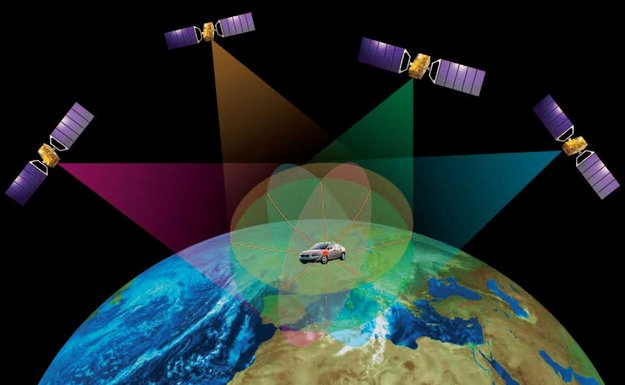
\includegraphics[width=0.6\textwidth]{pictureNav}
		\caption{Satelitska navigacija\cite{ref:34} }
		\label{Fig:nn}
		
	\end{figure}
	%http://www.academia.edu/12873735/PRIMJENA_GPS_GLOBALNI_NAVIGACIJSKI_SISTEM_i_GNSS_GLOBALNI_NAVIGACIJSKI_SATELITSKI_SISTEM_U_GEOLO%C5%A0KOM_KARTIRANJU_I_IZRADI_IN%C5%BDENJERSKO-GEOLO%C5%A0KIH_KARATA_NA_PRIMJERU_KLIZI%C5%A0TA_JUNUZOVI%C4%86I_SREBRENIK
	%primjena u kartografiji
	Koristeći pojam GNSS, najčešće se misli na \textit{sazviježđe}
	satelita koji odašilju signale potrebne za određivanje trenutnog položaja (i/ili brzine i vremena) i dodatne informacije u obliku tzv.\textit{Navigacijske poruke} (engl. Navigation Message (NM)).
	\textit{Sazviježđe} satelita predstavlja (1) svemirski segment GNSS sustava.
	U sastavnice GNSS-a spadaju i (2) kontrolni segment koji čine kontrolne i promatračke stanice smještene na Zemlji i (3) korisnički segment, odnosno GNSS prijamnici (slika \ref{Fig:GNSSsegmenti}).
	Kontrolni segment nadzire i upravlja radom sustava.
	
	\begin{figure}[H]
			\centering
			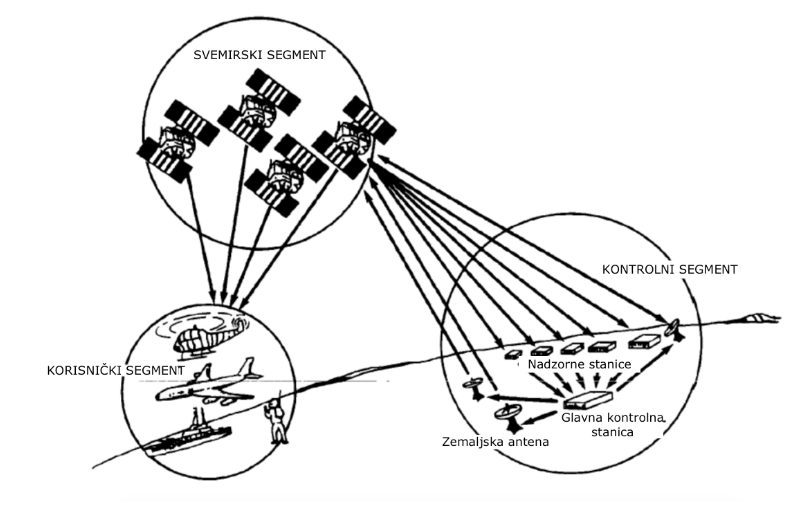
\includegraphics[width=0.6\textwidth]{GNSSsegmenti}
			\caption{Segmenti GNSS-a (GNSS)} %https://dr.nsk.hr/islandora/object/fpz%3A511/datastream/PDF/view
			\label{Fig:GNSSsegmenti}
			
	\end{figure}
	
	Trenutno postoji nekolicina GNS sustava (GNSS). Neki su u potpunosti 
	operativni, a neki samo djelomično.
	Najraširaniji u civilnoj upotrebi je GPS (Global Positioning System).
	GPS je u potpunosti operativan i u vlasništnu Vlade SAD-a. Njime upravlja Ministarstvo obrane SAD-a (engl. US Department of Defense).
	GPS omogućava dvije znatno različite razine korištenja, civilnu i vojnu.
	Vojna razina korištenja pruža više mogućnosti i točnije određivanje PVT stanja, a dopuštena je samo povlaštenim 
	korisnicima. Civilna razina korištenja je dostupna svima, bez dodatne naknade, uz uvjet posjedovanja GPS prijamnika. 
	
	Drugi, također u potpunost operativan GNSS, je GLONASS (Global'naya Navigatsionnaya Sputnikovaya Sistema) u vlasništvu Rusije.
	Neki od GNSS sustava u razvoju su: (1) Galileo i (2) BeiDou.
	Galileo-om upravlja Europska unija (EU). Najavljeno je da će postati u potpunosti operativan do 2020 \cite{ref:34}.
	BeiDou je kineski lokalni navigacijski satelitski sustav. U procesu je projekt proširenja BeiDou-a do globalnog do 2020 \cite{ref:34}.
	
	\begin{table}[H]
		\caption{Obilježja različitih satelitskih navigacijskih sustava}
		%\rowcolors{1}{}{lightgray}
		\begin{center}
			\begin{tabular}{|lllll|}
				\hline
				\rowcolor{lightgray}&  &  & &  \\
				\rowcolor{lightgray}&  &  & &  \\
				 \multirow{-3}{1cm}{ \cellcolor{lightgray}	} & \multirow{-3}{2cm}{\cellcolor{lightgray} Zemlja} & 
				 \multirow{-3}{2cm}{ \cellcolor{lightgray}Broj operativnih satelita} & \multirow{-3}{3cm}{\cellcolor{lightgray} Frekvencije valova nosilaca} & \multirow{-3}{3cm}{\cellcolor{lightgray} Brzina slanja navigacijske poruke} \\
				\hline\hline
				GPS & SAD & 31 & {L1 = 1575.42}
				& 50, 25 \\
				 &  &  & L2 = 1227.60 &  \\
				 &  &  & L5 = 1176.45 &  \\
				\hline
				GLONASS & Rusija & 28 & {L1 = oko 1602}
				& 50 \\
				 &  &  & L2 = 1246 &  \\
				 &  &  &&  \\
				\hline
				Beidou & NR Kina & 22 & {B1 = 1575.42}
				& - \\
				&  &  & B2 = 1191.795 &  \\
				&  &  & B3 = 1268.52 &  \\
				\hline
				Galileo & EU & 18 & {E1 = 1575.42}
				& - \\
				&  &  & E5a-Q = 1176.45 &  \\
				&  &  & E5b-Q = 1207.14 &  \\
				&  & \multirow{-3}{2.5cm}{(15 potpuno operativnih)} & E6 = 1278.75 &  \\
				\hline
			\end{tabular}
		\end{center}
		\label{tab:multicol}
	\end{table}
	
	Primjena GNSS-a dijeli se na pozicioniranje i navigaciju.
	\begin{defn}[Navigacija]
		Navigacija obuhvaća trenutno određivanje položaja i brzine entiteta u pokretu.
		Svrha navigacije je praćenje i upravljanje gibanja entiteta.
	\end{defn}
	
	\begin{defn}[Pozicioniranje]
		Pozicioniranje nazivamo postupak određivanja položaja točkovnog entiteta ili niza 
		točkovnih entiteta u prostoru.
	\end{defn}
	Ovim radom se ponajprije razmatra bespojena (engl. off-line) navigacijska primjena, u svrhu praćenja objekta (entiteta).
	Bespojena navigacija se koristi u prometnoj znanosti u analizi prometnih puteva. Kako ne zahtjeva izračunavanje u realnom vremenu (engl. real-time),
	svodi se na određivanje položaja točkovnog entiteta koji je statičan u danom vremenu $t$.
	Određujući položaj entiteta za niz vremena $ t_1,t_2, \hdots ,t_n $, dobiva se 
	aproksimacija kretanja entiteta u vremenskom okviru $[t_1,t_n]$.
	Preciznost aproksimacije kretanja zadaje se veličinom okvira i parametrom $n$, ili dostupnošću podataka.
	Praksa ne zathjeva da je $n$ u odnosu na vremenski okvir duljine 1 sata prevelik.
	Točno kretanje entiteta moguće je
	odrediti preslikavanjem dobivene aproksimacije na kartu prometnih puteva.
	U tu se svrhu koriste otprije poznati algoritmi.
	Dakle, rad se temalji na algoritamu za pozicioniranje (statičkog entiteta)
	u konceptu jednog, određenog, GNSS-a: GPS u aspektu civilne razine korištenja.
	
	Cilj rada je opisati, analizirati i izvesti osnovni (referentni) algoritam za pozicioniranje (statičkog entiteta), uvidjeti potencijalne slabosti te predložiti, izvesti i opravdati\footnote{Korsiti se komparativna analiza obilježja predloženog i izvornog algoritma koristeći eksperimentalno prikupljene pseudo-udaljenosti.} njegovo poboljšanje.
	Pod poboljšanjem se prvenstveno misli na poboljšanje u točnosti procjene položaja.
\end{intro}
%BIBL do kraja ispraviti , renato poslao kako	
\chapter[Globalni pozicijski sustav (GPS)][GPS]{Globalni pozicijski sustav (GPS, engl. Global Positioning System)}
	Sazvježđe GPS-a se sastoji od najmanje 24 satelita raspoređenih u 6 jednako odmaknutih orbita, svaka s inklanacijom od $55$ stupnjeva od ekvatorijalne
	ravnine.
	Sateliti kruže na visini od oko 20200 kilometara od Zemljine površine u srednje visokoj orbiti oko Zemlje (engl. Medium Earth Orbit (MEO)) s periodom rotacije 12 zvjezdanih sati. 
	Sateliti su raspoređeni na način da u svakom trenutku za svako mjesto na Zemljinoj površini postoje barem 4 dostupna satelita. Definicija dostupnosti satelita je dana u kasnijem teksu (Stranica \pageref{stranica:dostupnost}).
	
	Svi GPS sateliti odašilju (radio)signale s istim frekvencijama valova nosilaca (slika \ref{Fig:GPSSignal}). 
	U satelitima, vrijeme je praćeno pomoću cezijevih satova koji se sinkroniziraju s univerzalnom GPS atomskom vremenskom skalom. Sinkronizacija se odvija u periodima.
	\begin{figure}[H]
		\centering
		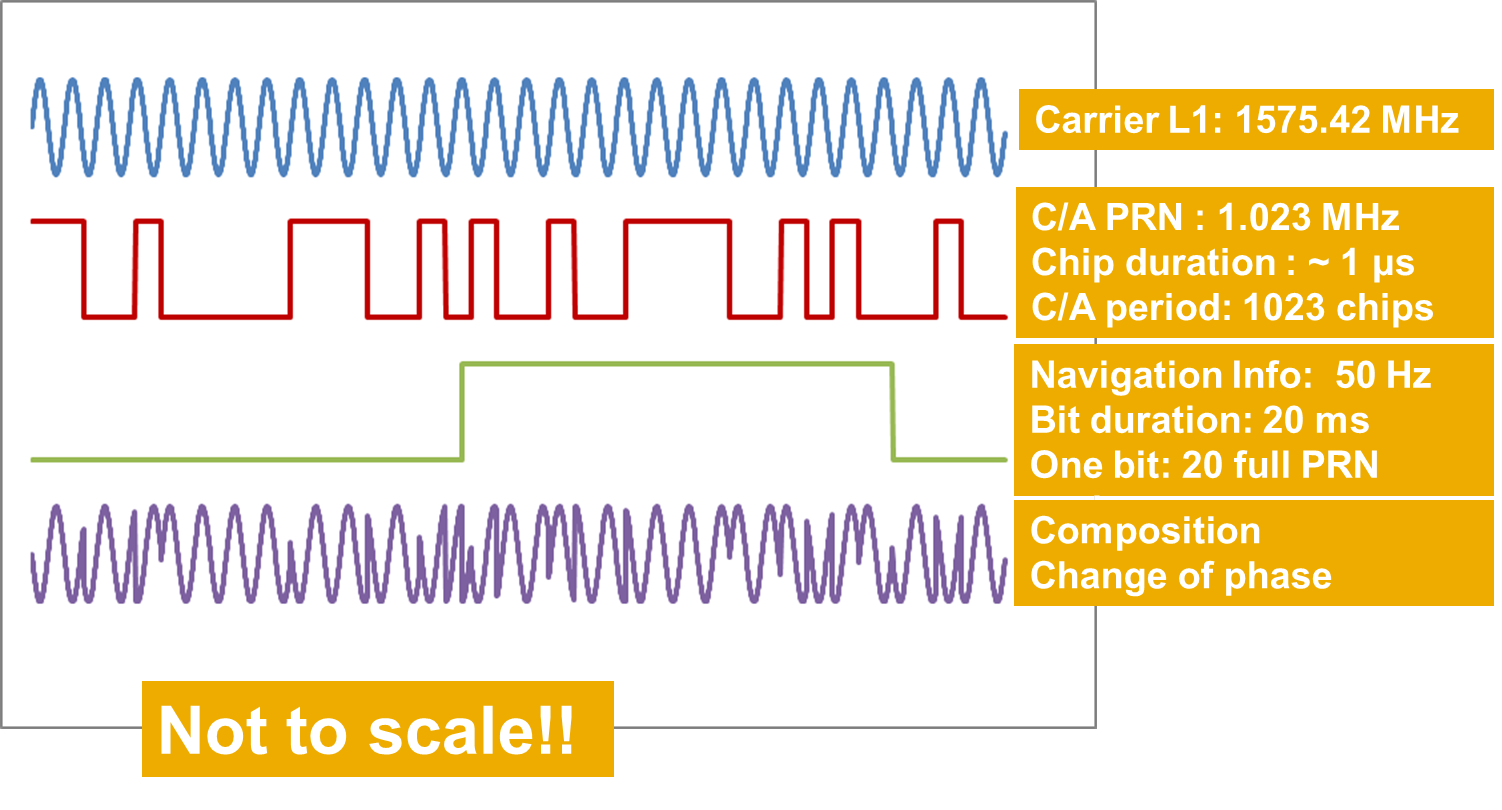
\includegraphics[width=0.4\textwidth]{GPS_Signals}
		\caption{GPS signal i njegove komponente \cite{GPS:1}}
		\label{Fig:GPSSignal}
	\end{figure}
	
	\section[C/A PRN kod]{GPS signali: C/A PRN i P kod}
	\subsection{C/A PRN kod i primjene}\label{CAkod}
	GPS sateliti odašilju signale na dvije frekvencije (vala nosilaca) $L_1$ i $L_2$, od kojih je $L_1$ na 1575.42 MHz namijenjena civilnoj upotrebi \footnote{Modificirani GPS koristi će i novu frekvenciju vala nosioca $L_5=1176.45 MHz$, a dio signala odašiljanih na $L_2$ također će biti dostupni i civilnim korisnicima.}. Pojam signal se često u satelitskoj navigaciji
	koristi samo za dio GPS signala koja sadržava C/A PRN kod (eng. Coarse Acquisition Pseudo Random Noise). 
	Svaki satelit koristi jedinstveni C/A PRN kod koji predstavlja niz 0 i 1 duljine 1023 bit-a.
	GPS-prijamnik razlikuje signale ( signale koji sadrže podatke potrebne za određivanje položaja i \textit{Navigacijske poruke}) različitih satelita
	temeljem sadržanih C/A PRN kodova. Satelit C/A PRN kodove odašilje neprestano, s početkom na početku svake sekunde. Prijemnik primljeni C/A PRN kod korsti za 
	razlikovanje satelita odašiljetelja, ali i za računanje pseudo-udaljenosti.
	
	\begin{defn}[Pseudo-udaljenost]
		Naka su svi sateliti numerirani prirodnim  brojevima s početkom 
		u 1. Neka je $\mathbf{S} \in \mathbb{N}$ neki satelit i $\mathbf{t}$ prijamnik
		koji je u mogućnosti primiti signal koji odašilje satelit $\mathbf{S}$. Pseudo-udaljenost
		između satelita odašiljatelja $\mathbf{S}$ i prijamnika primatelja $\textbf{t}$:
		$$d_s = c\cdot(t'_s- t_s)$$
		gdje je c konstanta koja je jednaka (prosječnoj) brzini putovanja signala od satelita do prijamnika. $t'_s$ je vrijeme primanja signala, a $t_s$ vrijeme slanja signala
		(po UTC vremenu).
	\end{defn}
	\textbf{Pseudo-udaljenost} je izmjerena udaljenosti (uz sadržane pogreške mjerenja) između satelita odašiljatelja i prijamnika primatelja signala u određenom trenutku.
	Vrijeme putovanja signala u oznaci $\Delta t := (t'_i- t_i)$, izračunava se poravnavanjem dijela primljenog signala (C/A PRN kod-a) i u prijemniku generiranog C/A PRN koda.
	Naime, prijamnik i satelit istovremeno generiraju isti C/A PRN kod. Cijelo vrijeme dok satelitski signal s generiranim
	C/A PRN kodom putuje, prijamnik nastavlja generanje istog C/A PRN koda. Po primitku signala,
	kodovi se poravnavaju. Temeljem razlike u poravnanju dobivenog i generiranog C/A PRN koda,
	mjeri se vrijeme putovanja satelitskog signala, tj. $\Delta t$ (slika \ref{fig:deltat}).
	\begin{figure}[H]
		\centering
		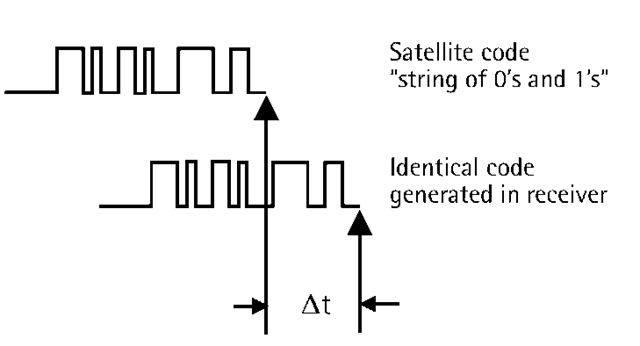
\includegraphics[width=0.4\textwidth]{deltat}
		\caption{Procjena vremena putovanja signala ($\Delta t$)}
		\label{fig:deltat}
	\end{figure}
	Za vrijednost konstante $c$ se uzima brzina svjetlosti u vakuumu koja predstavlja brzinu putovanja radiovala (poruke satelita) u vakuumu. Ona dovoljno dobro modelira stvarnu prosječnu brzinu putovanja. Naime, satelitski signal približno 90 posto puta se nalazi u uvjetima vakuuma.
	Budući da se psudo-udaljenost dobiva poravnavanjem kodova\label{stranica:kodno},
	upravo opisani način određivanja pseudo-udaljenosti naziva se kodni.
	
	Postoji još i fazni način određivanja psudo-udaljenosti koji se zasniva na poravnanju valova nosilaca (engl. Carrier phase) nakon micanjem C/A PRN i P(Y) kodova  iz poruke (GPS signala) \cite{fazno:kodno}.
	Fazno mjerenje služi kao nadopuna kodnom mjerenju u svrhu poboljšanja točnosti određivanja položaja.
	
	
	\section{P kod}\label{Pkod}
	P kod je dio GPS signala koji se odašilje na obje frekvencije i rezerviran je za vojnu razinu upotrebe.
	Kao i C/A PRN kod, sastoji se od karakterističnog pseudo-slučajnog niza nula i jedinica i šalje se brzinom 1023 bit/s. Znatno je dulji.
	Potrebno je ukupno 37 tjedana kako bi se sekvencijalno poslao cjelokupni P kod.
	Za razliku od C/A koda, gdje svaki satelit ima svoj jednistveni C/A kod, P kod je
	distribuiran među satelitima. Isječci P koda koji pripadaju različitim satelitima međusobno su različiti.
	Svakih 7 dana u točno određeno vrijeme određeni satelit odašilje svoj dio P koda.
	Na taj način, prijamnik razlikuje pojedinačne satelite. Npr. ukoliko
	satelit $\mathnormal{S}$ odašilje 14. tjedan P koda, onda je satelit $\mathnormal{S}$
	zapravo \textit{Space Vehicle 14 (SV 14)}.
	Kako bi se rezerviralo korištenje P koda samo za vojnu razinu upotrebe,
	prijamnik signalom ne prima goli P kod, već njegovu kriptiranu verziju, u oznaci $P(Y)$.
	Također, samo korisnicima s vojnom razinom upotrebe se prosljeđuje informacija kako dekriptirati $P(Y)$ u $P$.
	$P$ kod omogućava točnije određivanje položaja entiteta.
	
	\section{Pogreške određivanja položaja i vrste}\label{sec:pogreske}
	Pogreške određivanja položaja se grubo dijele na dvije vrste: (1)
	pogreške nastale uslijed konstrukcije ulaza algoritma i
	(2) uslijed primjene algoritma za određivanje položaja na mjerenim pseudo-udaljenostima.
	Dakle, postoje dva izvora: ulazni podatci algoritma (tip 1) i algoritam (tip 2).
	Najčešći izvori pogreške tipa 1 su pogreške pri određivanju pseudo-udaljenosti
	ili raspoređenost satelita oko Zemlje (Slike \ref{fig:DOP}, \ref{fig:DOPLow} i \ref{fig:DOPHigh}).
	Dvije skupine utjecajnih veličina (izvori pogrešaka tipa 1) nazivamo:%
	\begin{itemize}
		\item korisnička razdioba pogrešaka (engl. User Equivalent Ranging Error, UERE) i 
		\item geometrijska degradacija točnosti (engl. Geometric Dilutation of Precision, GDOP).
	\end{itemize}
	Budući da se gornje utjecajne veličine smatraju statistički neovisnima, ukupna pogreška 
	uslijed djelovanja izvora pogreška tipa 1 dobiva se kao $$P_{err_1} = UERE \times GDOP.$$
	
	Nepovoljan položaj promatranih satelita može rezultirati i zavisnim jednadžbama
	sustava jednadžbi za procjenu položaja pomoću satelita. Takvo što može onemogućiti procjenu položaja. U jednostavnijim slučajevima događa se povećanje GDOP-a, a time i ukupna pogreška određivanja položaja.
	\begin{figure}[H]
		\centering
		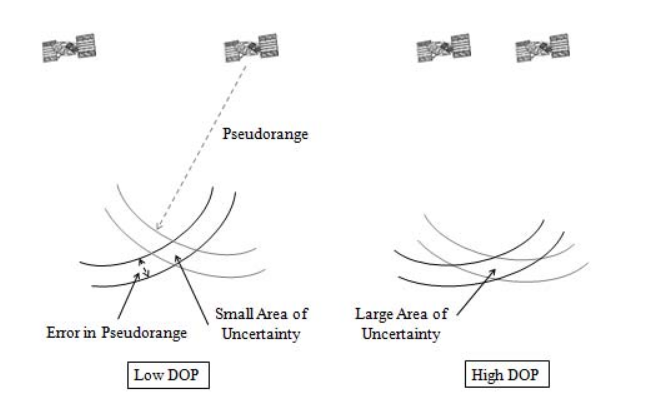
\includegraphics[width=0.6\textwidth]{DOP}
		\caption{Razlike u razmještaju satelita}
		\label{fig:DOP}
	\end{figure}%
	\begin{figure}[H]
		\centering
		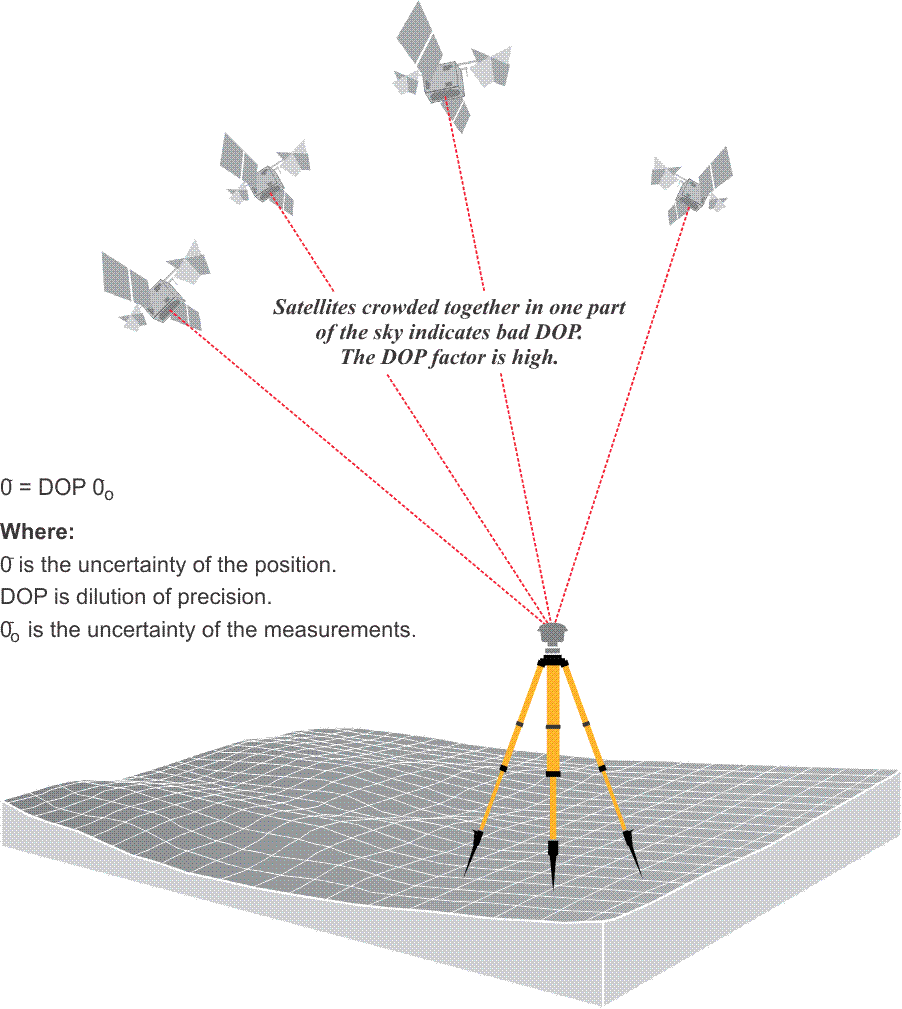
\includegraphics[width=0.6\textwidth]{DOPLow}
		\caption{Nepovoljan razmještaj satelita}
		\label{fig:DOPLow}
	\end{figure}%
	\begin{figure}[H]
		\centering
		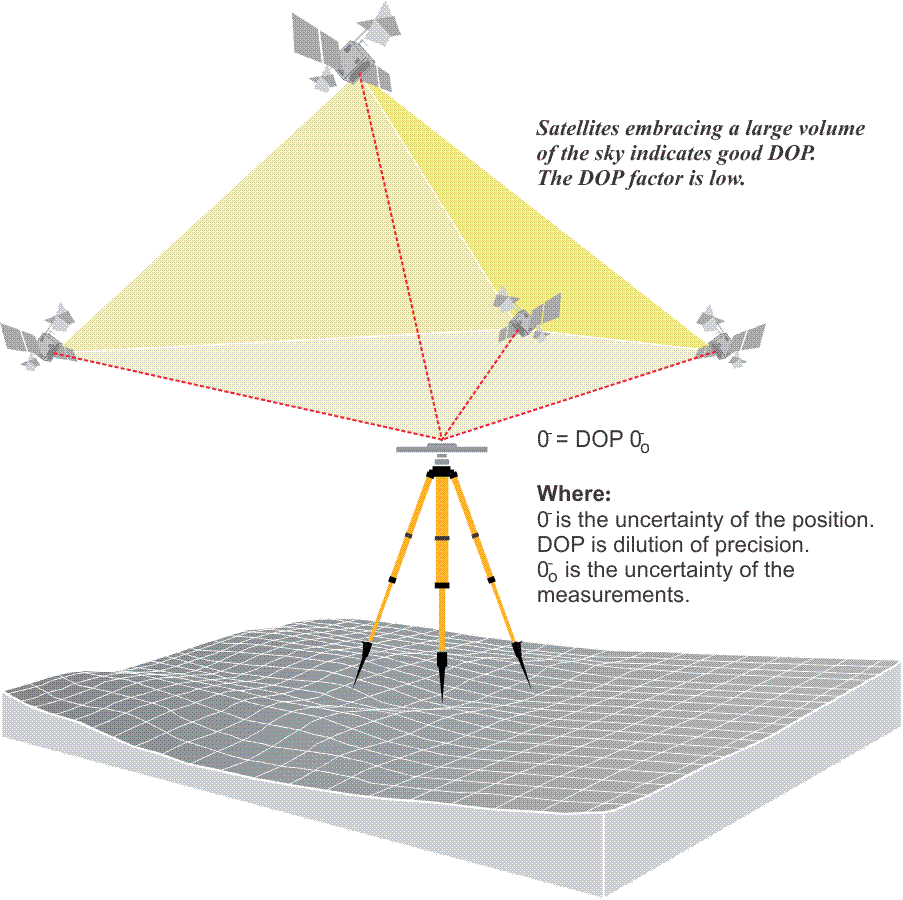
\includegraphics[width=0.4\textwidth]{DOPHigh}
		\caption{Povoljan razmještaj satelita}
		\label{fig:DOPHigh}
	\end{figure}
	
	
	
	Detaljnija podjela pogrešaka tipa 1 nastalih 
	pri određivanju psudo-udaljenosti (UERE pogreške) i područje utjecaja dano je sljedećom tablicom.
	
	\begin{table}[H]\centering
		\caption{Izvori i utjecaj pogreške tipa 1 na određivanje pseudo-udaljenosti}
		\begin{tabular}{ |p{3cm}|p{4cm}| }
			\hline
			\rowcolor{lightgray} Izvor & Utjecaj \\[0.5ex]
			\hline\hline
			\multirow{2}{4em}{satelit} & pogreške orbite  \\ 
			& pogreška sata satelita   \\ 
			\hline
			\multirow{2}{4em}{rasprostiranje signala} & troposferska refrakcija  \\ 
			& ionosferska refrakcija  \\
			\hline
			\multirow{4}{4em}{prijamnik} & pogreške antene  \\ 
			& pogreška sata\\ 
			%OVO je tip 2
			%& pogreška pojednostavljena računalnih
			%postupaka (tip 2)\\
			\cline{2-2}
			& pogreška višestaznih puteva \\
			\hline
		\end{tabular}
	\end{table}	
	
	One mogu biti sistemske ili slučajne. %KOJA JE RAZLIKA?
	Utjecaj sistemskih pogrešaka otklanja se modeliranjem ili
	kombinacijom opažanja.
	Korištenjem više prijamnika, otklanjaju se pogreške spacifične za satelite.
	Pogreške specifične za prijamnike otkanja korištenje većeg broja satelita od
	potrebnog broja za određivanje položaja.
	Utjecaje troposfere je najsigurnije otkloniti modeliranjem,
	a ionosfere korištenjem dva signala različitih frekvencija.
	Nažalost, ponekad nije moguće korištenje dva signala različitih frekvencije
	pa se i utjecaj ionosfere otkanja modeliranjem. Ukoliko se utjecaj ionofere otklanja
	modeliranjem, uvijek ostaje dio slučajne pogreške utjecaja ionosfere
	koja se može uzeti u obzir prilikom izgradnje algoritma za određivanje položaja
	u navigacijskoj domeni (Poglavlje \ref{sec:algTezine}).
	
	Slučajne pogreške nastaju zbog trenutnog mjerenja, slučajnog dijela
	višestruke refleksije signala (engl. multipath) nastalog interferencijom 
	direktnog i reflektiranog signala (slika \ref{fig:multipath}) te zbog slučajnog karaktera ionosferskog kašnjena koji se ne ispravlja sistemskim modelom.
	\begin{figure}[H]
		\centering
		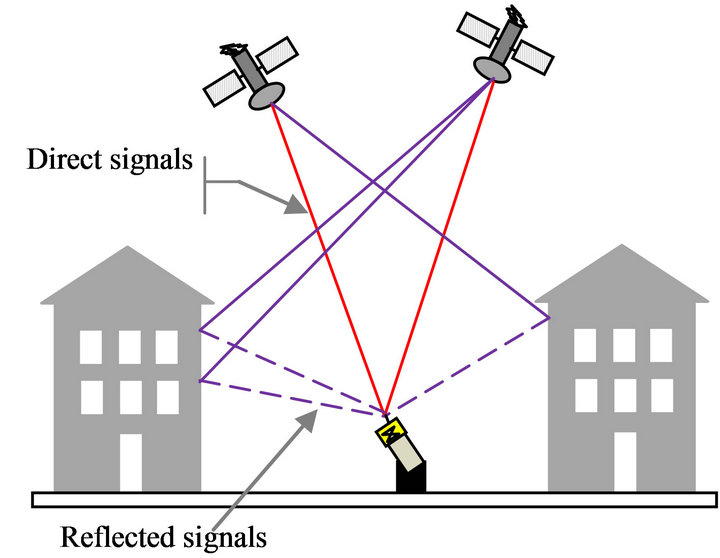
\includegraphics[width=0.4\textwidth]{multipath}
		\caption{Višestruka refleksija signala}
		\label{fig:multipath}
	\end{figure}
	
	U poglavlju \ref{sec:izvedba} prvo se izvodi osnovni algoritam za određivanje položaja 
	prijamnika koji polazi od pretpostavke o potpunoj ispravljenosti pseudo-udaljenosti\label{stranica:greskaOvisisamoOxOpravdano}.
	Kasnije, uvođenjem težinskih koeficijenata (Poglavlje \ref{sec:algTezine}), reducira se utjecaj pogrešaka
	psudo-udaljenosti.
%	Sistemske pogreške lako se otklanjaju otklonjene koristeći RTK-LIB <- ali ja to modeliram.
%	%RTK LIB u POGLAVLJE 4).
%	 Prije konstrukcije ulaza algoritma za određivanja položaja, smatramo da je
%	pogreška s izvorom u pseudo-udaljenostima maksimalno reducirana.
%	Dakle, pretpostavljamo kako ona više nije značajna
%	neuzimajući ju u obzir u daljnjem postupku izračuna položaja. \label{stranica:greskaOvisisamoOxOpravdano}
%	Smatramo da koristimo potpuno ispravljene pseudo-udaljenosti.
	
	\vspace{0.5cm}
	Pogreške tipa 2 mogu imati izvor u konstrukciji (dizajnu) izvedbe algoritma ili njegovoj izvedbi, npr.
	numeričke greške, greške zbog ograničene preciznosti računala,
	aproksimacije pojedinih vrijednosti.
	
	One se ne modeliraju algoritmima procjene položaja (poglavlje \ref{sec:algoritam}), već prilikom konstrukcije izvedbe odabranog algoritma (poglavlje \ref{sec:izvedba})
 	
	%U poglavlju \ref{sec:izvedba}, biti će obrađena analiza pogreške tipa 2 za odabrani algoritam.
	
	\section{Navigacijska poruka}\label{sec:NM} %http://what-when-how.com/gps/gps-details/
	Svaki satelit, uz C/A PRN i P kod, odašilje i dodatne podatke potrebne za ispravo određivanje položaja prijamnika. Odašilje ih u obliku \textit{Navigacijske poruke} koja se šalje zajedno s generiranim C/A PRN kodovima (slika \ref{Fig:GPSSignal}).
	
	Navigacijska poruka se sastoji od 25 okvira \cite{ref:34}.
	Jedan okvir se sastoji od 5 podokvira i svaki sadržava vrijeme slanja
	sljedećeg okvira (slika \cite{GPS:1}). Za slanje cjelokupnog podokvira potrebno je 6 sekundi,
	6 cjelokupnih C/A PRN kodova. Prijemnik je u mogućnosti računati pseudo-udeljenost za novi položaj satelita svakih
	6 sekundi.
	Za slanje cjelokupne NM, potrebno je 12.5 minuta.
	U nastavku teksta, naziv poruka koristi se sa značenjem podprozora.
	\vspace{0.5cm}
	
	Prozor sadrži:
	\begin{enumerate}
		\item GPS vremena odašiljanja,
		\item signal prijenosa s P na C/A kod (potpoglavlja \ref{Pkod} i \ref{CAkod}),
		\item podatke o orbitalnoj putanji satelita,
		\item podatke o korekciji sata satelita,
		\item almanah statusa svih satelita u sazvježđu,
		\item koeficijente preračunavanja GPS vremena u UTC,
		\item parametre standardnog GPS ionosferskog modela korekcija.
	\end{enumerate}
	
	\begin{defn}[Universal Time Coordinate (UTC vrijeme)]
		Universal Time Coordinate je vremenski standard zasnovan na međunarodnom atomskom vremenu koji se najčešće koristi u znanstvene i vojne svrhe. \footnote{Drugi nazivi za taj vremenski standard su ZULU vrijeme i Greenwich Mean Time (GMT)}.
	\end{defn}
	
	\begin{figure}[H]
		\centering
		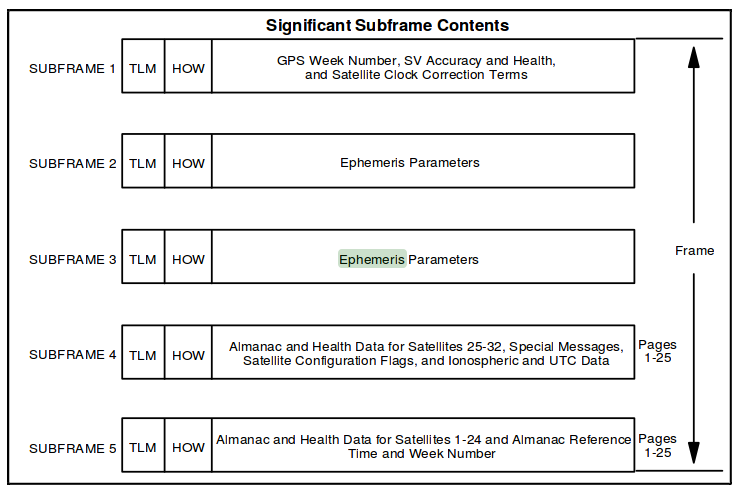
\includegraphics[width=0.6\textwidth]{NACONTENT}
		\caption{Pregled strukture prozora navigacijske poruke\cite{GPS:1}}
		\label{Fig:aaa}
	\end{figure}
	Pojedini dijelovi navigacijske poruke pomažu pri otklanjaju pogrešaka tipa 1  
	(poglavlje \ref{sec:pogreske}), određivanju
	pseudo-udaljenosti i trenutnom položaju satelita.
	Naime, iz podataka o orbitalnoj putanji satelita moguće je za odabrani trenutak izračunati koordinate položaja satelita referentnom koordinatnom sustavu pa i svakom drugom.
	 
	Za potrebe ovoga rada, dovoljno je razumjeti sljedeće.
	Prijemnik svakih 6 sekundi ima dovoljno podataka da izmjeri novu pseudo-udaljenost do istog satelita sve dok on ne prestane biti dostupan. 
	
	\begin{defn}[Dostupnost satelita $\mathnormal{S}$ prijamniku $\mathnormal{T}$]
		\label{stranica:dostupnost}
		Za satelit $\mathnormal{S}$ kažemo da je dostupan prijamniku $\mathnormal{T}$ u trenutku $\mathnormal{t}$ ako je u sljedećih 6 sekundi u mogućnosti izmjeriti
		pseudo-udaljenost do satelita $\mathnormal{S}$ i konstruirati sljedeću jednadžbu:
		\begin{align}\label{eq:position1}
		d_s = \sqrt{(x-x_s)^{2}+(y-y_s)^{2}+(z-z_s)^{2}}
		\end{align}
		gdje su jedine nepoznanice $(x,y,z)$, tj. koordinate položaja prijamnika.
		$(x_s,y_s,z_s)$ su poznate koordinate položaja satelita. 
	\end{defn}
	
	\section{Proces određivanja položaja}\label{sec:positionProcess}
	U pravilu, u svakom trenutku, prijamnik ima više dostupnih satelita od kojih dobiva poruke. Za određivanje položaja prijamnika u granicama dopuštene točnosti,
	zahtjevaju se barem 4 dostupna satelita\label{stranica:4satelita}.
	
	Kako bi prijamnik odredio svoj položaj računa tri nepoznate koordinate položaja koje su obično izražene jednom od sljedećih koordinatnih sustava:
	\begin{enumerate}
		\item geodetskom koordinatnom sustavu koji je izveden referentnim ECEF XYZ koordinatnim sustavom,
		\item geografskom koordinatnom sustavu koji koristi koordinate jednake geografskoj širini, duljini i nadmorskoj visini.
	\end{enumerate}
	% odnosno koordinate u trodimenzionalnom pravokutnom koordinatnom sustavu (geoprostornom koordinatnom sustavu) \textit{WGS84}.
	% Geoprostornom koordinatni sustav \textit{WGS84} pred
	
	Neka je $k$ broj vidljivih satelita od prijamnika $\mathnormal{T}$.
	Prijemnik $\mathnormal{T}$ promatrajući poruke dobivene od samo jednog satelita,
	u vremenu $\mathnormal{t}$, izračunava samo jednu pseudo-udaljenost i može konstruirati samo jednu jednadžbu \ref{eq:position1}
	 koja mu omogućava odrediti sferu oko promatranog satelita na kojoj bi se mogao nalaziti (slika \ref{Fig:1SatelitePosition}).
	
	\begin{figure}[H]
		\centering
		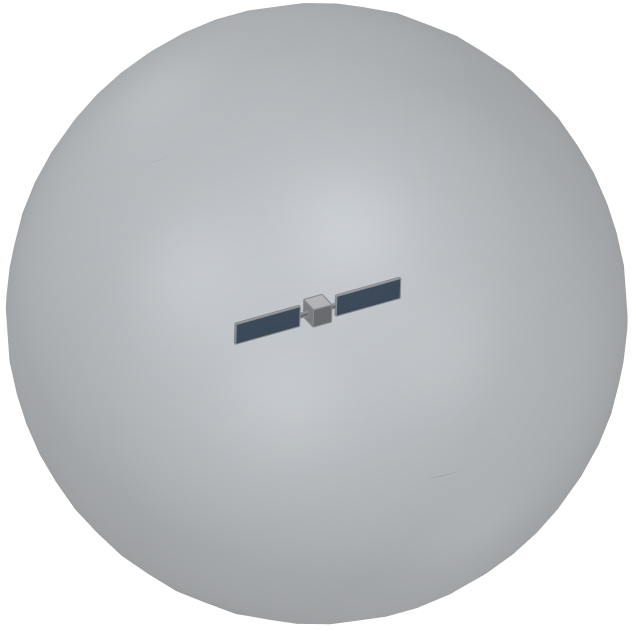
\includegraphics[width=0.4\textwidth]{satellite_distance_13D}
		\caption{Sfera oko promatranog satelita na kojoj bi se prijamnik mogao nalaziti \cite{gps:2}}
		\label{Fig:1SatelitePosition}
	\end{figure}
	Uključujući u izračun pridobivene pseudo-udaljenosti još jednog satelita dobivamo situaciju prikazanu na Slici \ref{Fig:2SatelitePosition}.
	\begin{figure}[H]
		\centering
		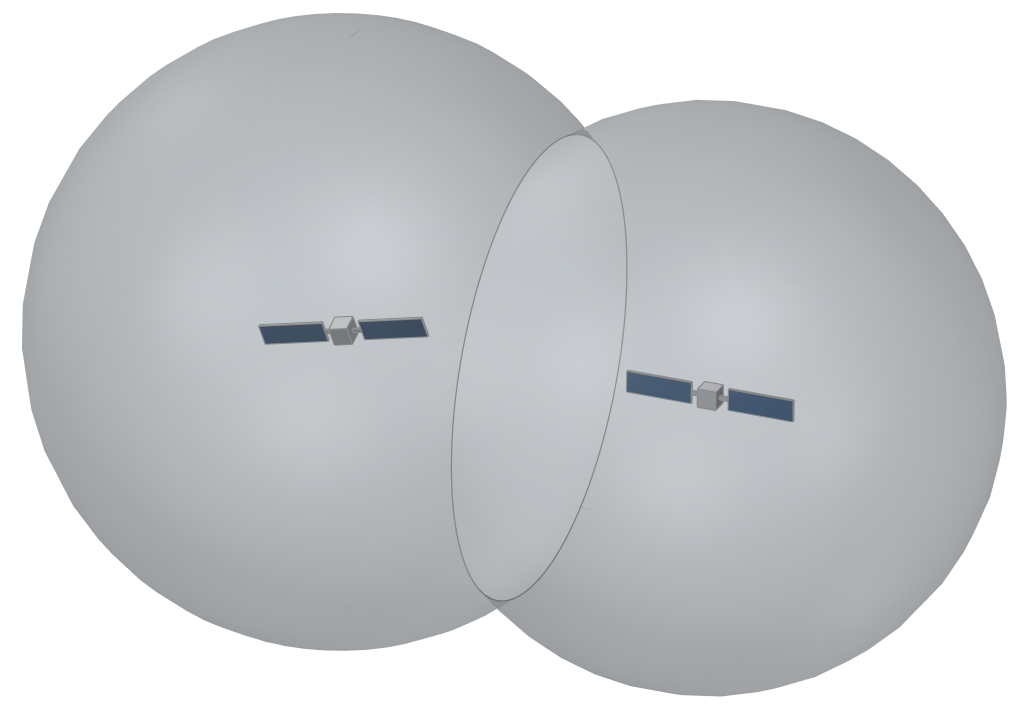
\includegraphics[width=0.6\textwidth]{satellites_distance_23D}
		\caption{Sfere oko dva promatrana satelita. Presjek je kružnica na kojoj bi se prijamnik mogao nalaziti. \cite{gps:2}}
		\label{Fig:2SatelitePosition}
	\end{figure}
	Uključujuči u izračun još jedan satelit, dobivamo situaciju prikazanu na Slici \ref{Fig:3SatelitePosition}.
	
	\begin{figure}[H]
		\centering
		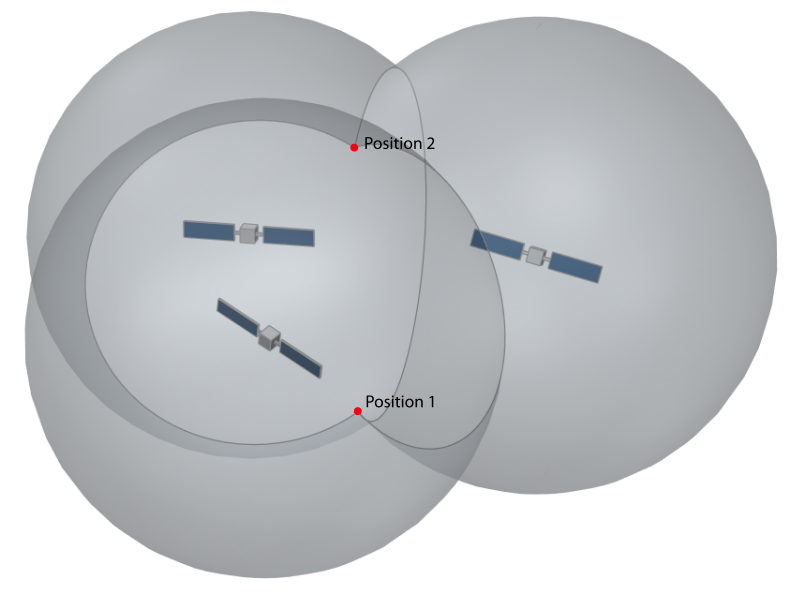
\includegraphics[width=0.6\textwidth]{satellites_distance_33D}
		\caption{Sfere oko tri promatrana satelita. Presjek su dvije točke na kojoj bi se prijamnik mogao nalaziti. \cite{gps:2}}
		\label{Fig:3SatelitePosition}
	\end{figure}
	
	Presjek tri promatrane sfere su dvije točke na kojoj bi se prijamnik mogao nalaziti.
	Jedna točka se nalazi daleko u svemiru, dok je druga točka točka kandidat položaja prijamnika. 
	
	Algebarski, rješavamo sljedeći sustav linearnih jednadžbi u $(x,y,z)$ :
	\begin{align}\label{eq:position2}
	 d_1 = \sqrt{(x-x_1)^{2}+(y-y_1)^{2}+(z-z_1)^{2}} \notag \\
	 d_2 = \sqrt{(x-x_2)^{2}+(y-y_2)^{2}+(z-z_2)^{2}} \\
	 d_3 = \sqrt{(x-x_3)^{2}+(y-y_3)^{2}+(z-z_3)^{2}} \notag
	\end{align}
	gdje su $1,2 \text{ i }3$,  3 različita satelita, a $(x_i,y_i,z_i)$ pripadajuće
	koordinate položaja satelita u referentnom ECEF XYZ (egl. Earth-Centered, Earth-Fixed XYZ) koordinatnom sustavu.
	ECEF XYZ koordinatni sustav ima ishodište u centru Zemljine mase od čega dolazi (engl. Earth-Centered).
	Sve tri osi (X,Y i Z) koje izlaze iz ishodišta usklađene su s rotacijom Zemlje, tj. rotiraju zajedno sa Zemljom (engl. Earth-Fixed).
	Z-os prolazi kroz sjeverni pol a XY osi definiraju ekvatorijalnu ravninu. \\
	Zbog kompleksnosti Zemljine površine, uzima se elipsa kao njezina aproksimacija.
	Trenutni referentni ECEF XYZ koordinatni sustav WGS84 koristi elipsu sljedećih parametara:%
	\begin{itemize}
		\item $a = 6378137$,
		\item $f = \frac{1}{298.257223563}$
	\end{itemize}
	i prikazan je slikom \ref{Fig:na}.
	
	
	\begin{figure}[H]
		\centering
		\begin{minipage}{0.45\textwidth}
			\centering
			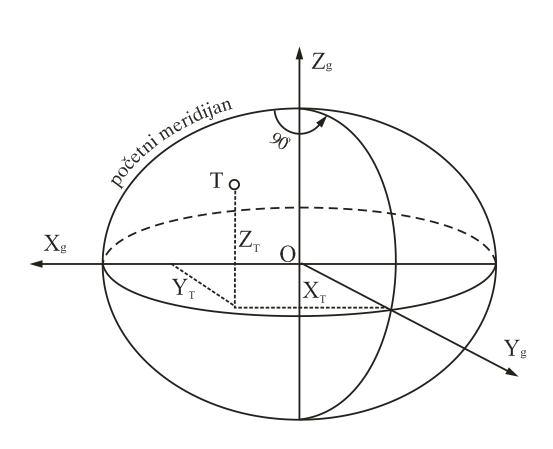
\includegraphics[width=0.6\textwidth]{ECEFcro.png}
			\caption{ECEF $\mathnormal{X}$, $\mathnormal{Y}$, $\mathnormal{Z}$ koordinatni sustav \cite{geo:slikeSustava}}
			\label{Fig:na}
		\end{minipage}%
		\hspace{0.5cm}
		\begin{minipage}{0.45\textwidth}
			\centering
			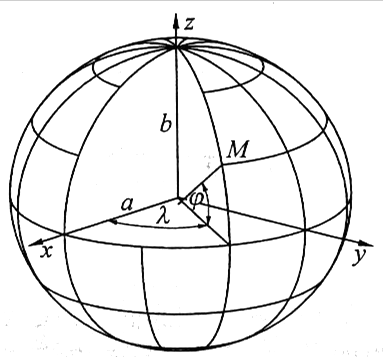
\includegraphics[width=0.6\textwidth]{GEOcro.png}
			\caption{Geografski koordinatni sustav \cite{geo:slikeSustava}}
			\label{Fig:na1}
		\end{minipage}
	\end{figure}
	
	Svaki prijamnik je sposoban izvesti konverziju iz i u koordinata u referentnom ECEF XYZ sustavu 
	u i iz geografskih (geografska širina, duljina i nadmorska visina) \cite{GPS:overview}.
	Dakle, prijamniku su potrebna barem 3 dostupna satelita kako bi odredio položaj.
	Ali se ipak na stranici \pageref{stranica:4satelita} se postavlja zahtjev na barem 4. 
	
	Primjetimo kako proces određivanja položaja prijamnika
	indirektno zahtjeva usklađenost satova prijamnika i dostupnih satelita.
	Satovi svih satelita su međusobno usklađeni usklađenošću stabilnih atomskih satova na satelitima s GPS vremenom. Ukoliko odstupanje ipak postoji, biti će zapisano u navigacijskoj poruci pa se može uzeti u obzir prilikom određivanja položaja prijamnika.
	Napomenimo, GPS vrijeme nije jednako UTC vremenu. GPS vrijeme je bilo 0 u 06.01.1980. i određeno je protjecanjem vremena u GPS satelitima, tj. njihovim 
	satovima. 
	
	Satovi prijamnika nisu iste preciznosti \footnote{Govorimo o preciznosti, tj. na koliko "decimala" je moguće odrediti vrijeme (koje možda i nije točno ako sat nije dobro usklađen).} kao satovi satelita.
	Prijemnici obično koriste satove preciznosti do otprilike $10^{-6}$ sekundi.
	Pogreška određivanja vremena od $10^{-6}$ sekundi dovodi do pogreške u
	određivanju pseudo-udaljenosti od oko 300 metara.
	Uz pogreške preciznoti sata prijemnika, postoje još pogreške sata prijemnika zbog neapsolutne sinkroniziranosti s GPS vremenom.
	Uključujući u izračun i obe pogreške sata prijamnika, pseudo-udaljenost modeliramo jednadžbom
	\begin{align}
	d_i = c\times(t'_i- t_i+ d_T)
	\end{align}
	gdje $d_T$ predstavlja spomenutu pogrešku korisničkog sata.
	Budući da se prilikom određivanja položaja, 
	spomenuta pogreška  u oznaci $d_T$ ne mijenja u odnosu na satelit koji se promatra,
	može se izračunati dodavajući ju kao nepoznanicu u sustav jednadžbi \ref{eq:position2}
	Dakle, sustav jednadžbi \ref{eq:position2} prelazi u:
	\begin{align}\label{eq:position3}
	d_1 = \sqrt{(x-x_1)^{2}+(y-y_1)^{2}+(z-z_1)^{2}} + c\cdot d_T \notag \\
	d_2 = \sqrt{(x-x_2)^{2}+(y-y_2)^{2}+(z-z_2)^{2}} + c\cdot d_T  \\
	d_3 = \sqrt{(x-x_3)^{2}+(y-y_3)^{2}+(z-z_3)^{2}} + c\cdot d_T \notag 
	\end{align}
	
	Kako bi za gornji sustav postojala mogućnost pronalaska rješenja,
	uvodi se zahtjev na još barem jedan dostupni satelit, što je ukupno 4 (Stranica \pageref{stranica:4satelita}).
	Dobivamo sljedeći sustav jednadžbi u $(x,y,z,d_T)$:
	\begin{align}\label{eq:1}
	 d_1 = \sqrt{(x-x_1)^{2}+(y-y_1)^{2}+(z-z_1)^{2}} + c\cdot d_T \notag \\
	 d_2 = \sqrt{(x-x_2)^{2}+(y-y_2)^{2}+(z-z_2)^{2}} + c\cdot d_T  \\
	 d_3 = \sqrt{(x-x_3)^{2}+(y-y_3)^{2}+(z-z_3)^{2}} + c\cdot d_T \notag \\
	 d_4 = \sqrt{(x-x_4)^{2}+(y-y_4)^{2}+(z-z_4)^{2}} + c\cdot d_T \notag
	\end{align}
	
	Upravo opisanom postupkom otklanjamo slučajnu pogrešku nastalu prilikom 
	određivanja pseudo-udaljenosti 
	s izvorom u pogrešci sata prijamnika.
	U praksi se može koristiti još veći broj dostupnih satelita što poboljšava 
	točnost određivanja položaja prijamnika. Očekivana pogreška rješenja dobivenog rješavanjem sustava \ref{eq:1} je veličina između $10^2$ i $10^4$ [m]. Tako dobiveno rješenje se profinjuje čime se postiže pogreška veličine $10^1$ [m] \footnote{Pofinjenje se obično obavlja kombiniranjem opažanja (modeliranjem nakon primjene algoritma procjene položaja u domeni navigacijske primjene) ili modelima ispravaka primjenjenim na mjerenim pseudo-udaljenostima (modeliranjem prije primjene algoritma procjene položaja u domeni navigacijeske primjene).}.
	Ovim radom se proučava, opisuje, oblikuje i izvodi algoritam za rješavanje sustava \ref{eq:1}.
	Naime, rješavanje sustava \ref{eq:1} čini temelj procesa određivanja položaja i nužno ga je provesti.
	U primjenama koje zahtjevaju relativno malu točnost, ono je i dovoljno.\\
	Metode za profinjavanje (poboljšanje) dobivenog rješenja (modeli ispravaka) mogu biti izrazito kompleksne i ovise o primjeni. Svojom kompleksnošću i raznovrsnošću prelaze obseg ovoga rada.\\

\chapter[Algoritam procjene položaja (APP)]{Algoritam procjene položaja u domeni navigacijske primjene}\label{sec:algoritam}
%Algoritam procjene položaja za ulazne podatke, ne mora nužno određivati nadmorsku visinu, geografsku širinu i duljinu. Postoji više geoprostornih koordinatnih sustava za određivanje
%pozicije objekta. Korištenje nadmorske visine, geografske širine i duljine predstavlja jedan geoprostorni koordinatni sustav. Ovisno o geoprostornom sustavu koordinata korištenih satelita, algoritam određuje geoprostorni koordinatni sustav u kojem će biti prikazana izračunata pozicija prijamnika. 
Postupak procjene položaja satelitskim navigacijskim sustavom traži ispunjavanje sljedećih preduvjeta:
\begin{itemize}
	\item Korištenje zajedničkog (geoprostornog) referentnog sustava,
	\item Korištenje zajedničkog vremena (vremenskog okvira) sustava,
	\item Ispunjavanje pretpostavke o pravocrtnom širenju satelitskih signala jedinstvenom
	brzinom (brzina svjetlosti u vakuumu).
\end{itemize}
Uvjeti trebaju biti ispunjeni od strane svih satelita odabranog/odabranih GNSS sustava, ali i korištenog prijamnika.
Prvi uvjet je uvijek lako ispuniti. Druga dva se ispunjavaju na razne načine:
(1) modeliranjem prije primjene algoritma za određivanje položaja u navigacijskoj domeni, (2)
korištenjem prekobrojih satelita ili prijamnika (vidi: poglavlje \ref{sec:positionProcess}), (3) modeliranjem prilikom primjene algoritma za određivanje položaja u navigacijskoj domeni (samim algoritmom), (4) modeliranjem nakon primjene algoritma za određivanje položaja u navigacijskoj domeni.
Modeliranje prije primjene algoritma za određivanje položaja u navigacijskoj domeni obuhvaća modele ispravaka mjerenih pseudo-udaljenosti, tzv. modeli ispravaka \footnote{Modeli ispravaka se nerjetko zasnivaju na dnevnim vijednostima parametra modela sadržanim u dnevnom almanahu.}.

Na primjer, odstupanje sata prijamnika od vremenskog okvira sustava modelira se kao četvrta nepoznanica sustava 
(vidi: poglavlje \ref{sec:positionProcess}).

\textit{Algoritmom procjene položaja u domeni navigacijske primjene} (APP)
smatramo svakim algoritmom koji za sustav jednadžbi \ref{eq:1}
određuje nepoznati položaj prijamnika u koordinatama $(x,y,z)$.
Broj jednadži sustava može biti i veći od 4. Tada govorimo o prezasićenom sustavu.
Ovisno o odabiru, APP se može temeljiti na rješavanju sustava nelinearnih jednadžbi pronalaženjem rješenja pomoću (1) metode najmanjih kvadrata (Newton-ova metoda),
(2) metode zatvorene forme, (3) metode najbližeg susjeda \cite{math:positioning}. 


Općenito, rješava se modificiran sustav jednadžbi \ref{eq:1} 
u koji uključejemo nepoznati parametar $(v_1,v_2,v_3,v_4)$, dodatnu pogreška
izračuna:
\begin{align}\label{eq:new}
d_1 = \sqrt{(x-x_1)^{2}+(y-y_1)^{2}+(z-z_1)^{2}} +d + v_1\notag \\
d_2 = \sqrt{(x-x_2)^{2}+(y-y_2)^{2}+(z-z_2)^{2}} +d + v_2 \\
d_3 = \sqrt{(x-x_3)^{2}+(y-y_3)^{2}+(z-z_3)^{2}} +d + v_3\notag \\
d_4 = \sqrt{(x-x_4)^{2}+(y-y_4)^{2}+(z-z_4)^{2}} +d + v_4\notag
\end{align}
gdje je $d = c \cdot d_T$.

Uz oznake 
\begin{align}
\mathbf{\rho} := (d_1, d_2, d_3, d_4)^T \\ 
\mathbf{x} := (x,y,z,d_T)^T \\ 
\mathbf{s}_i := (x_i,y_i,z_i)^T \\ 
\mathbf{h} (\mathbf{x}) := 
\begin{bmatrix}\label{eq:hx}
||(s_1-\mathbf{x}_{1:3})|| + x_4\cdot c\\
||(s_2-\mathbf{x}_{1:3})|| + x_4\cdot c\\
||(s_3-\mathbf{x}_{1:3})|| + x_4\cdot c\\
||(s_4-\mathbf{x}_{1:3})|| + x_4\cdot c
\end{bmatrix} \\
\mathbf{v} := (v_i,v_2,v_3,v_4)^T \label{eq:v}
\end{align}%
\ref{eq:new} prelazi u
\begin{align}\label{eq:matrix}
\mathbf{\rho} = \mathbf{h}(\mathbf{x})+\mathbf{v}
\end{align}%
\section{Iterativna metoda najmanjih kvadrata}

Primjetimo kako je $\mathbf{h}(\mathbf{x})$ definiran s \ref{eq:hx} jednak vektoru udaljenosti
satelita i prijamnika za prave vrijednosti $\mathbf{x}$, $\bar{\mathbf{x}}$ i pogrešku sata $d_T$ = 0.\\


Općenito oblikovanje algoritma za određivanje položaja u domeni navigacijske primjene nema utjecaj na
pogreške tipa 2,
već samo pogreške tipa 1 (Stranica \pageref{stranica:greskaOvisisamoOxOpravdano}).
Također, pretpostavlja se kako su otklonjene sve pogreške tipa 1 koje imaju izvor 
u pogreškama izračuna pseudo-udaljenosti (osim pogreški sata prijamnika) (Stranica \pageref{stranica:greskaOvisisamoOxOpravdano}).
Ostaje još samo modelirati pogreške koje imaju za izvor trenutni položaj satelita dostupnih za
izračunavanje željenog položaja $\bar{\mathbf{x}}_{(1:3)}$.
U tu svrhu modeliramo vektor pogrešaka $\mathbf{v}$, funkcijom $\mathbf{p}(\mathbf{x})$ koja ovisi o nepoznatom parametru $\mathbf{x}$.
Uz oznaku $\mathbf{y} := \mathbf{\rho}$, 
 jednadžba  \ref{eq:matrix} prelazi u
\begin{align}\label{eq:matrix2}
\mathbf{y} = \mathbf{\rho} = \mathbf{h}(\mathbf{x})+ \mathbf{p}(\mathbf{x})
\end{align}%
Preciznije,
član $\mathbf{p}(\mathbf{x})$ modelira pogrešku razlike u procjeni parametra $\mathbf{x}$ od stvarne vrijednosti.
Što je aproksimacija potrebnih vrijednosti za izračun rješenja matrične jednadžbe
\ref{eq:matrix} točnija, to je $\mathbf{p}(\mathbf{x})$ 
bliže nuli za pravu vrijednost $\bar{\mathbf{x}}$.
Aproksimaciju za $\bar{\mathbf{x}}$, u oznaci $\hat{\mathbf{x}}$, pronalazimo tražeći nultočke funkcije $\mathbf{p}(\mathbf{x})$.
U praksi je uobičajeno da mjerenja sadrže pogreške i tada $\mathbf{p}(\mathbf{x})$ uopće ne mora imati 
nultočke i $\hat{\mathbf{x}}$ ne možemo pronaći tražeći nultočke funkcije $\mathbf{p}(\mathbf{x})$.

Konceptualno, ideja metode najmanjih kvadrata je pronalaženje $\hat{\mathbf{x}}$ traženjem minimuma
funkcije $\mathbf{p}(\mathbf{x})$, tj.
\begin{align}\label{eq:minimization}
	\hat{\mathbf{x}} := \text{arg min}_\mathbf{x} \mathbf{p}(\mathbf{x})^T\mathbf{p}(\mathbf{x})
\end{align}
Problem opisan jednadžbom \ref{eq:minimization} nije linearan pa
ne postoji općeniti način pronalaska njegovog rješenja.

U slučaju kada su funkcija koju treba minimiziati i početna vrijednost $\mathbf{x}_0$
(iterativnog postupka) dovoljno dobre 
%(vidi: dodatak \ref{appendix:aTay})
, rješenja problema \ref{eq:minimization} moguće je
dobiti iterativnim postupakom.
Ideja iterativnog postupka je, počevši s $\mathbf{x}_0$, računati $\mathbf{x}_1, \mathbf{x}_2, \hdots $ sve dok se novoizračunate vrijednosti ne prestanu mijenjati ili postanu dovoljno bliske prethodnoj, tj.
$\left \| x_{k} - \mathbf{x}_{k-1}\right\| < \delta$ za dovoljno male $\delta > 0$.
$\delta$ još nazivamo i zaustavni kriterij.

Prikladni iterativni postupak rješavanja problema \ref{eq:minimization} je Newton-Gaussova metoda (iterativna metoda najmanjih kvadrata).
Newton-Gaussova metoda linearizira $\mathbf{p}(\mathbf{x})$ u okolini od $\mathbf{x_k}$ pomoću prvog člana razvoja funkcije u Taylorov red\label{stranica:NGLin} u točki $\mathbf{x}_k$:
\begin{align}\label{eq:approx}
	\mathbf{p}(\mathbf{x_k}+ \Delta \mathbf{x_k}) \approx \mathbf{p}(\mathbf{x_k}) + \mathbf{p}'(\mathbf{ x_k})\cdot \Delta \mathbf{x_k}
\end{align}

$\Delta \mathbf{x_k}$ se odabire na način tako da
$$lim_{k \to \infty} \left( \mathbf{p}(\mathbf{x_k}) \right) = 0$$ 
jer za pravu vrijednost $\mathbf{x}$ izraz $\mathbf{p}(\mathbf{x}) = 0$ ili poprima svoj minimum ukoliko postoje pogreške
točnosti vrijednosti koje se koriste prilikom konstrukcije sustava.
 
Sada, za $\mathbf{p}(\mathbf{x_{k+1}}) := \mathbf{p}(\mathbf{x_k}+ \Delta \mathbf{x_k}) \approx \mathbf{p}(\mathbf{x_k}) + \mathbf{p}'(\mathbf{x_k})\cdot \Delta \mathbf{x_k}$ želimo
 da je što bliže 0.
 Dakle, $ \Delta \mathbf{x_k} $ odabiremo trežeći minimum funkcije
\begin{align}\label{eq:minDelta}
	\mathbf{p}(\mathbf{x_k}) + \mathbf{p}'(\mathbf{x_k})\cdot \Delta \mathbf{x_k}
\end{align}
u $\Delta \mathbf{x_k}$.

Označimo sada s $\mathbf{J}_k := \mathbf{p}'(\mathbf{x_k}) = \mathbf{h}'(\mathbf{x_k})$.
\ref{eq:minDelta} prelazi u 
\begin{align}\label{eq:minDelta2}
	\mathbf{J}_k \Delta \mathbf{x_k} +\mathbf{p}(\mathbf{x_k})
\end{align}
čij je minimun dan s (Stranica \pageref{stranica:nastavakLS})  
\begin{align}\label{eq:minDeltaRj}
\Delta \mathbf{x_k} = - (\mathbf{J}_k^T\mathbf{J}_k)^{-1}\mathbf{J}_k^T \mathbf{p}(\mathbf{x_k})
\end{align}

Izraz za $\mathbf{x_{k+1}}$ je sljedeći:
\begin{align}\label{eq:iter}
	\mathbf{x_{k+1}} = \mathbf{x_{k}} - (\mathbf{J}_k^T\mathbf{J}_k)^{-1}\mathbf{J}_k^T \mathbf{p}(\mathbf{x_k})
\end{align}
Prilikom izvedbe algoritma, potrebano je primjereno odrediti početnu vijednost $\mathbf{x_0}$, te kasnije iterirati po formuli \ref{eq:iter}.
Uz odabir prikladanog $\mathbf{x}_0$, dovoljno blizu rješenju i
ako je druga derivacija od $\mathbf{p}$ u točki $\bar{\mathbf{x}}$ dovoljno mala,
niz $x_0,x_2, \hdots$ konvergira prema $\bar{\mathbf{x}}$. Izračun $\mathbf{J}_k$ za idealan slučaj $d = 0$ se može naći u prilogu \ref{appendix:aTay}.

Algoritam iterativne metode najmanjih je dan u nastavku.

\begin{algorithm}[H]
	\KwData{ $\mathbf{p(\mathbf{x})}, \mathbf{x}_0, \delta$ }
	\KwResult{ $\hat{\mathbf{x}} $ }
	$k = 0$ \;
	\While{$ \left \| \mathbf{x}_{k} - \mathbf{x}_{k-1}\right\| \geq \delta $}{
		$\mathbf{J}_k = \mathbf{p}'(\mathbf{x}_k)$ \;
		$\Delta \mathbf{x}_k = - \mathbf{J}_k^{-1} \cdot \mathbf{p}(\mathbf{x}_k) $ \;
		$\mathbf{x}_{k+1} =\mathbf{x}_k + \Delta \mathbf{x}_k$ \;
	$k ++$\;
	} 
	$\hat{\mathbf{x}} = \mathbf{x_k}$
\caption{Iterativna metoda najmanjih kvadrata}
\label{algorithm:iterLSM}
\end{algorithm}

Prilikom korištenja gornjeg algoritma za određivanje položaja objekta, za $\mathbf{x}_0$ se mogu uzeti koordinate središta zemlje jer su jednadžbe za određivanje položaja dovoljno bliske linearnima.

Ako je poznato da su vrijednosti koje koristimo za konstrukciju
jednadžbi za određivanje položaja \ref{eq:1} za pojedine jednadžbe točnije,
prirodno je pridjeliti im prednost pred ostalima.
Važnost pojedine jednadžbe modeliramo pridavanjem težina pojedinoj jednadžbi.
Jednadžbi se pridružuje težina $\sigma_i$ koja je proporcionalna preciznosti 
vrijednosti korištenih prilikom njezine konstrukcije.
Najčešće način pronalaženja odgovarajućih težina je
korištenjem kovarijancone matrice
vektora pogrešaka $\mathbf{v}$ (Jednadžba \ref{eq:v}),u oznaci $\Sigma : = cov(\mathbf{v})$. Minimizacijski problem \ref{eq:minimization} prelazi u %
\begin{align}\label{eq:minimisation2}
\hat{\mathbf{x}} = \text{arg min}_\mathbf{x} \mathbf{p}(\mathbf{x})^T \Sigma^{-1} \mathbf{p}(\mathbf{x})
\end{align}%
Sada, algoritam \ref{algorithm:iterLSM} prelazi u algoritam \ref{algorithm:iterLSMW}.

\begin{algorithm}[H]
	\KwData{ $\mathbf{p(\mathbf{x})}, \mathbf{x}_0, \delta$, $\Sigma$ }
	\KwResult{ $\hat{\mathbf{x}} $ }
	$k = 0$ \;
	\While{$ \left \| \mathbf{x}_{k} - \mathbf{x}_{k-1}\right\| \geq \delta $}{
		$\mathbf{J}_k = \mathbf{p}'(\mathbf{x}_k)$ \;
		$\Delta \mathbf{x}_k = - (\Sigma^{-\frac{1}{2}}\mathbf{J}_k ) ^{-1} ( \Sigma^{-\frac{1}{2}}(\mathbf{p}(\mathbf{x}_k))$ \;
		$\mathbf{x}_{k+1} =\mathbf{x}_k + \Delta \mathbf{x}_k$ \;
		$k ++$\;
	} 
	$\hat{\mathbf{x}} = \mathbf{x_k}$
	\caption{Iterativna metoda težinskih najmanjih kvadrata}
	\label{algorithm:iterLSMW}
\end{algorithm}
Procjenitelj za $\bar{\mathbf{x}}$ dobiven težinskom metodom najmanjih kvadrata, jednakost \ref{eq:minimisation2}, ima najmanju varijancu među svim procjeniteljima za
$\bar{\mathbf{x}}$. Ukoliko je vektor pogrešaka $\mathbf{v}$ normalno
distribuiran, procjenitelj \ref{eq:minimisation2} postaje procjenitelj
metode najbližeg susjeda (podpoglavlje \ref{sec:MLE} i MLE procjenitelj).

Prilikom korištenja iterativne metode najmanjih kvadrata potrebno je
modelirati distribuciju vektora pogrešaka, točnije kovarijanconu matricu $\Sigma$.
Također, potrebno je pripazati na 
velike pogreške u određivanju vrijednosti pomoći kojih se gradi sustav jednadžbi 
\ref{eq:1} i netipične vrijednosti (engl. outliners) koji se uklanjaju prije primjene algoritma.

Sljedeće poglavlje opisuje izvedbu upravo opisanog algoritma \ref{algorithm:iterLSMW} i 
analizu njegove točnosti. Prije same izvedbe, navodi se zanimljiva posljedica
analize pogreške metode najmanjih kvadrata i pregled još nekih metoda za rješavanje
sustava \ref{eq:1}.
\subsection{Analize pogreške metode najmanjih kvadrata}
Uz oznake kao do sada, neka $\bar{\mathbf{y}}$ predstavlja prave udaljenosti između satelita i promatranog objekta (prijamnika) i $\hat{\mathbf{y}}$ izračunate pseudo-udaljenosti. 
Vrijedi
$\hat{\mathbf{y}} = \bar{\mathbf{y}} + \Delta \mathbf{y}$.
Promotrimo idealan slučaj za metodu iterativnih najmanjih kvadrata (algoritam \ref{algorithm:iterLSM}) gdje je $\delta = 0$.
Neka je $\hat{\mathbf{x}} = \bar{\mathbf{x}} + \Delta \mathbf{x}$ rješenje dobiveno metodom najmanjih kvadarata, tj. 
$\hat{\mathbf{x}} = \mathbf{x}_{k'}$ i $\forall m \geq k', \mathbf{x}_m = \mathbf{x}_{m+1}$.
Uvrštavanjem $\mathbf{x}_k = \hat{\mathbf{x}}$ i $\mathbf{y} = \hat{\mathbf{y}}$ u jednadžbu \ref{eq:iter} dobivamo
\begin{align*}
	\mathbf{x_{k+1}} &= \mathbf{x_{k}} - (\mathbf{J}_k^T\mathbf{J}_k)^{-1}\mathbf{J}_k^T \mathbf{p}(\mathbf{x_k}) \\
	\mathbf{x_{k+1}} - \mathbf{x_{k}} &= - (\mathbf{J}_k^T\mathbf{J}_k)^{-1}\mathbf{J}_k^T \mathbf{p}(\mathbf{x_k}) \\
	0 &= - (\mathbf{J}_k^T\mathbf{J}_k)^{-1}\mathbf{J}_k^T \mathbf{p}(\bar{\mathbf{x}} + \Delta \mathbf{x}) \\
	0 &= (\mathbf{J}_k^T\mathbf{J}_k)^{-1}\mathbf{J}_k^T (\mathbf{h}(\bar{\mathbf{x}} + \Delta \mathbf{x}) -(\bar{\mathbf{y}} + \Delta \mathbf{y}))\\
\end{align*}
Matrica $\mathbf{J}_k$ predstavlja funkciju koja ovisi o parametru $\mathbf{x}$. Ona nije konstantna.
Kako 
se pretpostavlja da je $\Delta \mathbf{x}$ dovoljno blizu nule, opravdano je smatrati $\mathbf{\mathbf{J}} := \mathbf{\mathbf{J}}_k$ konstantom za susjedstvo od $\bar{\mathbf{x}}$ radijusa $\Delta \mathbf{x}$.
Sada se $\mathbf{h}$ u okolini točke $\bar{\mathbf{x}}$ može linearizirati na sljedeći način:
$$\mathbf{h}(\mathbf{x}+\delta) = \mathbf{h}(\mathbf{x}) + \mathbf{J} \delta, \delta > 0$$.\\
Dobivamo
\begin{align*}
0 &= (\mathbf{J}^T\mathbf{J})^{-1}\mathbf{J}^T (\mathbf{h}(\bar{\mathbf{x}}) + \mathbf{J}\Delta \mathbf{x} -(\bar{\mathbf{y}} + \Delta \mathbf{y}))\\
0 &= (\mathbf{J}^T\mathbf{J})^{-1}\mathbf{J}^T (\mathbf{J}\Delta \mathbf{x} - \Delta \mathbf{y})\\
(\mathbf{J}^T\mathbf{J})^{-1}\mathbf{J}^T \mathbf{J}\Delta \mathbf{x}& = (\mathbf{J}^T\mathbf{J})^{-1}\mathbf{J}^T \Delta \mathbf{y}\\
\Delta \mathbf{x} &= (\mathbf{J}^T\mathbf{J})^{-1}\mathbf{J}^T \Delta \mathbf{y}\\
\end{align*}
Uz pretpostavku normalnosti pogreške izračunavanja pseudo-udaljenosti,
\newline $\Delta \mathbf{y} \sim N(0,\Sigma)$, imamo
\begin{align}\label{eq:xerrorDistr}
	\Delta \mathbf{x} \sim N(0,(\mathbf{J}^T\mathbf{J})^{-1}\mathbf{J}^T\Sigma \mathbf{J}(\mathbf{J}^T\mathbf{J})^{-1})
\end{align}
Uz $\Sigma = \sigma^2I$, $\Delta \mathbf{x} \sim N(0,\sigma^2(\mathbf{J}^T\mathbf{J})^{-1})$.
U kontekstu satelitske navigacije, $(\mathbf{J}^T\mathbf{J})^{-1}$ nazivamo DOP (engl. Dilution of Precision) matricom.
Iz DOP matrice moguće je izvesti različite mjere kvalitete sazviježđa satelita u danom trenutuku za dani položaj.
\begin{enumerate}
	\item GDOP = $\sqrt{tr(\mathbf{J}^T\mathbf{J})^{-1}}$
	\item PDOP = $\sqrt{tr((\mathbf{J}^T\mathbf{J})^{-1}_{(1:3,1:3)})}$
	\item HDOP = $\sqrt{tr((\mathbf{J}^T\mathbf{J})^{-1}_{(1:2,1:2)})}$
	\item VDOP = $\sqrt{(\mathbf{J}^T\mathbf{J})^{-1}_{(3,3)}}$
	\item TDOP = $\sqrt{(\mathbf{J}^T\mathbf{J})^{-1}_{(4,4)}}$
\end{enumerate}
Opširnije o mjerama kvalitete sazviježđa moguće je naći u dodatku \ref{appendix:DOP} ovomu radu.

Dakle, uz neke pretpostavke, iz Jakobijeve matrice funkcije $\mathbf{h}$, $J$, može se saznati mnogo o kvaliteti 
određivanja položaja za sustav jednadžbi \ref{eq:1}, veličini pogreške određivanja
s izvorom u kvaliteti "zviježđa".
Izračuni gornjih mjera su točni onoliko koliko su pretpostavke
o jednakosti varijance za $\Delta \mathbf{y}$ i $\Delta \mathbf{x}$
istinite.

Primjenu metode najmanjih kvadrata moguće je pronaći na stranici \pageref{stranica:nastavakLS}.

\section{Metoda zatvorene forme}
Metoda zatvorene forme pronalazi izravno rješenje sustava \ref{eq:1} \cite{math:positioning}.
Za razliku od iterativnih metoda,
metode zatvorene forme ne zahtjevaju postavljanje početnog rješenja $\mathbf{x}_0$ i uvjeta zaustavljanja $\delta$. Rješenje je egzaktno i ne postoji mogućnost 
pronalaska krivog rješenja (lokalnog minimuma). Ukoliko postoji više rješenja sustava, 
zatvorena forma pronalazi sve.

Budući da se metodama zatvorene fome otežano modeliraju pogreške mjerenja,
one se ne koriste za pronalazak krajnjeg rješenja sustava.
Ipak,
zatvorena forma je korisna u pronalasku početnog rješenja sustava iterativnog postupka, istraživanje, razvoj i grafičko predočavanje.


Za mjerene psudoudaljenosti $y_1,y_2, \hdots y_n$ i nepoznatu pogrešku sata prijamnika $x_4$, rješenje 
problema najmanjih kvadrata danog jednadžbama
\begin{align}\label{eq:zatvorena1}
y_1 &= \left \| \mathbf{s}_1 - \mathbf{x}_{1:3} \right \| + \mathbf{x}_{4} \notag \\
y_2 &= \left \| \mathbf{s}_2 - \mathbf{x}_{1:3} \right \| + \mathbf{x}_{4} \notag \\
y_2 &= \left \| \mathbf{s}_3 - \mathbf{x}_{1:3} \right \| + \mathbf{x}_{4} \\
&\vdots \notag \\
y_n &= \left \| \mathbf{s}_n - \mathbf{x}_{1:3} \right \| + \mathbf{x}_{4} \notag 
\end{align}
u $x_{1:3}$ i $x_4$ dano je sljedećim zatvorenim formama
\begin{align}\label{eq:zatvorena2}
	\mathbf{x}_{1:3} = \mathbf{d}\lambda + \mathbf{e} \\
	\mathbf{x}_{4} = f\lambda + g \notag
\end{align}
gdje $\lambda$ dobivamo rješavanjem sljedeće jednadžbe
\begin{align}
	( \left \|\mathbf{d}\right \|^2 - f^2 ) \lambda^2 + (2\mathbf{d}^T \mathbf{e} - 2fg - 1)\lambda + \left \|\mathbf{e}\right \| - g^2 = 0.
\end{align}
 $\hat{\mathbf{x}}$ je rješenje sustava \ref{eq:zatvorena1} ako i samo ako je
rješenje zatvorene forme \ref{eq:zatvorena2}.

Parametre $\mathbf{d}$, $\mathbf{e}$, $f$ i $g$ zatvorene forme \ref{eq:zatvorena2} dobivamo iz sustava \ref{eq:zatvorena1}
sljedećim nizom pretvorbi: \\

\begin{align}
(y_1 -x_4)^2 &= \left \| \mathbf{s}_1 - \mathbf{x}_{1:3} \right \|^2 \notag \\
(y_2 -x_4)^2 &= \left \| \mathbf{s}_2 - \mathbf{x}_{1:3} \right \|^2 \notag \\
(y_3 -x_4)^2 &= \left \| \mathbf{s}_3 - \mathbf{x}_{1:3} \right \|^2 \\
&\vdots \notag \\
(y_n -x_4)^2 &= \left \| \mathbf{s}_n - \mathbf{x}_{1:3} \right \|^2 \notag 
\end{align}
\begin{align}
y_1^2 -2y_1 x_4 + x_4^2 &= \left \| \mathbf{s}_1\right \|^2 -2\mathbf{s}_1^T\mathbf{x}_{1:3} +\left\|  \mathbf{x}_{1:3} \right \|^2 \notag \\
y_2^2 -2y_2 x_4 + x_4^2 &= \left \| \mathbf{s}_2\right \|^2 -2\mathbf{s}_2^T\mathbf{x}_{1:3} +\left\|  \mathbf{x}_{1:3} \right \|^2 \notag \\
y_3^2 -2y_3 x_4 + x_4^2 &= \left \| \mathbf{s}_3\right \|^2 -2\mathbf{s}_3^T\mathbf{x}_{1:3} +\left\|  \mathbf{x}_{1:3} \right \|^2 \\
&\vdots \notag \\
y_n^2 -2y_n x_4 + x_4^2 &= \left \| \mathbf{s}_n\right \|^2 -2\mathbf{s}_n^T\mathbf{x}_{1:3} +\left\|  \mathbf{x}_{1:3} \right \|^2 \notag 
\end{align}
Uz \begin{align}
	\lambda := \left\| \mathbf{x_{1:3}}\right \|^2 - x_4^2
\end{align}
dobivaju se linearne jednadžbe u $\mathbf{x_{1:3}}$, $x_4$ i $\lambda$
\begin{align}
	-\lambda+y_i^2 - \left \| \mathbf{s}_i\right \|^2 = 2y_i x_4 - 2\mathbf{s}_i^T \mathbf{x}_{1:3} 
\end{align}
koje čine sustav
\begin{align}
\begin{bmatrix}
2\mathbf{s}_1^T & -2y_1 \\
2\mathbf{s}_2^T & -2y_2 \\
2\mathbf{s}_3^T & -2y_3 \\
\vdots \\
2\mathbf{s}_n^T & -2y_n 
\end{bmatrix}
\begin{bmatrix}
\mathbf{x}_{1:3} \\
x_4
\end{bmatrix} =
\begin{bmatrix}
1 \\
1 \\
1 \\
\vdots \\
1 
\end{bmatrix} \lambda + 
\begin{bmatrix}
\left \| \mathbf{s}_1\right \|^2 & -y_1^2\\
\left \| \mathbf{s}_2\right \|^2 & -y_2^2\\
\left \| \mathbf{s}_3\right \|^2 & -y_3^2\\
\vdots \\
\left \| \mathbf{s}_n\right \|^2 & -y_n^2
\end{bmatrix}.
\end{align}
Naposljetku, za
\begin{align}
	\begin{bmatrix}
	\mathbf{d} \\
	f
	\end{bmatrix}:=
	\mathbf{p} = \begin{bmatrix}
	2\mathbf{s}_1^T & -2y_1\\
	2\mathbf{s}_2^T & -2y_2 \\
	2\mathbf{s}_3^T & -2y_3\\
	\vdots \\
	2\mathbf{s}_n^T & -2y_n
	\end{bmatrix}^T 
	\begin{bmatrix}
	1 \\
	1 \\
	1 \\
	\vdots \\
	1 
	\end{bmatrix} 
	\\ 
	\begin{bmatrix}
	\mathbf{e} \\
	g
	\end{bmatrix}:=
	\mathbf{q} = \begin{bmatrix}
	2\mathbf{s}_1^T & -2y_1\\
	2\mathbf{s}_2^T & -2y_2 \\
	2\mathbf{s}_3^T & -2y_3\\
	\vdots \\
	2\mathbf{s}_n^T & -2y_n
	\end{bmatrix}^T
	\begin{bmatrix}
	\left \| \mathbf{s}_1\right \|^2 & -y_1^2\\
	\left \| \mathbf{s}_2\right \|^2 & -y_2^2\\
	\left \| \mathbf{s}_3\right \|^2 & -y_3^2\\
	\vdots \\
	\left \| \mathbf{s}_n\right \|^2 & -y_n^2
	\end{bmatrix}
\end{align}
dobivamo \ref{eq:zatvorena2}.

\section{Metoda najbližeg susjeda (maksimalne vjerodostojnosti)}\label{sec:MLE}
Metode najbližeg susjeda opisuju pogrešku mjerenja uvjetnom vjerojatnošću,
$\mathbf{p}(y|\mathbf{x})$.
$\mathbf{p}(y|\mathbf{x})$ je vjerojatnost da je psudoudaljenost $y$ izmerena na položaju
s koordinatama $\mathbf{x}_{1:3}$ s pogreškom u izvoru sata prijamnika jednakoj $\mathbf{x}_4$ \cite{math:positioning}.
Ukoliko se $\mathbf{x}$ postavi za varijablu, a $y$ za konstantu, dobivamo
funkciju maksimalne vjerodostojnosti (ML), u oznaci
$L(\mathbf{x}|Y) =\mathbf{p}(y|\mathbf{x})$.

Za problem određivanja položaja opisanog
jednadžbom \ref{eq:matrix}, lako se dobiva ekvivalentan problem određivanja položaja
 maksimalne vjerodostojnosti.
Budući da vrijedi:
\begin{align}
\mathbf{v} = \mathbf{\rho}-\mathbf{h}(\mathbf{x})
\end{align}%
i $\mathbf{v}$ je poznate distribucije, dobivamo:
\begin{align}\label{eq:ML}
\mathbf{p}( y|\mathbf{x_{1:3}} ) = \mathbf{p_v} \left(\mathbf{\rho}-\mathbf{h}(\mathbf{x_{1:3}}) \right)
\end{align}

Ukoliko je problem određivanja položaja zadan s \ref{eq:ML},
$\hat{\mathbf{x}}$ pronalazimo pomoću procjenitelja maksimalne vjerodostojnoti za $\mathbf{x}$, tj. $\hat{\mathbf{x}}$ je takav da vrijedi
\begin{align}
	L(\hat{\mathbf{x}} | y) := \max_{\tilde{\mathbf{x}}} (L(\tilde{\mathbf{x}} | y)) 
\end{align}
gdje $\tilde{\mathbf{x}}$ predstavljaju sve dozvoljene 
koordinate položaja objekta na Zemlji i u zraku.

Za poznata mjerenja psudoudaljenosti, $\hat{\mathbf{x}}$ se može pronaći metodom nelinearne optimizacije \cite{math:positioning}.\\
Metoda najbližeg susjeda i metoda težinskih najmanjih kvadrata daju isto rješenje za  $\hat{\mathbf{x}}$ uz normalnu distribuiranost vektora $\mathbf{v}$ i matrice težina postavljene na $\Sigma^{-1} = cov(\mathbf{v})^{-1}$.
Naime, za:
\begin{align*}
\mathbf{p}_v (\mathbf{z}) = C \exp \left(-\frac{1}{2} \mathbf{z}^T \Sigma^{-1} \mathbf{z}\right) \\
C = (2\pi)^{-\frac{n}{2}}det (\Sigma)^{-\frac{1}{2}}
\end{align*}
dobiva se:
\begin{align}\label{eq:MLeq}
\mathbf{p}( y|\mathbf{x} ) = \mathbf{p_v} \left(\mathbf{\rho}-\mathbf{h}(\mathbf{x}) \right)
= C \exp \left(-\frac{1}{2} (\mathbf{\rho}-\mathbf{h}(\mathbf{x}) )^T \Sigma^{-1} (\mathbf{\rho}-\mathbf{h}(\mathbf{x}) )\right)
\end{align}
Budući da je $\Sigma$ pozitivno definitna matrica, argument eksponencijalne funkcije gornjeg izraza je uvijek negativan.
Dakle, problem maksimizacije funkcije \ref{eq:MLeq} jednak je minimizaciji
izraza:
\begin{align}
(\mathbf{\rho}-\mathbf{h}(\mathbf{x}) )^T \Sigma^{-1} (\mathbf{\rho}-\mathbf{h}(\mathbf{x}) = \mathbf{v}^T \Sigma^{-1}\mathbf{v} = 
\mathbf{p}^T (\mathbf{x}) \Sigma^{-1}\mathbf{p} (\mathbf{x}).
\end{align}


Dakle, $\hat{\mathbf{x}} = \text{arg min}_x \left( \mathbf{p}^T (\mathbf{x}) \Sigma^{-1}\mathbf{p} (\mathbf{x}) \right)$ 
što odgovara izrazu \ref{eq:minimisation2} uz matricu težina jednaku $cov(\mathbf{v})^{-1}$.

\chapter{Programski određen GPS prijamnik}
Za pokretanje izvedbe procesa određivanja položaja, potrebno je prvo prikupiti podatke koji će biti korišteni. Potrebne podatke je moguće prikupiti u \textit{RINEX} obliku 
koristeći civilni programski određen GPS prijamnik praktično izveden na vlastitom računalu ili 
koristeći podatke s međunarodne GNSS referentne postaje (engl. International GNSS Service reference station, IGS reference station).
Kako bi se formulirali podatci potrebni za ulaza izvedenog procesa određivanja položaja
željenog formata, potrebno je obraditi prikupljene \textit{RINEX} podatke i prebaciti u željeni oblik, tekstualnu datoteku s 1 (pseudo-udaljenosti) ili 3 stupca podataka (x,y i z koordinate položaja satelita u ECEF XYZ koordinatama \footnote{WGS84 koordinatama}).\\
Obradu prikupljenih \textit{RINEX} podatka je moguće napraviti koristeći
programski određen GPS prijamnik praktično izvedenog na vlastitom računalu.

\section{Model programski određenog radioprijamnika}
Svaki radioprijamnik obavlja procesiranje signala i informacija u četiri osnovne domene:
\begin{itemize}
	\item domena pretvorbe elektromagnetskog vala u električni signal (u anteni),
	\item domena visokih (radijskih) frekvencija, u kojoj se obrađuje primljeni modulirani signal te obavlja demodulacija i prijenos u osnovno frekvencijsko područje,
	\item domena osnovnog frekvencijskog područja, u kojoj se procesiraju signali nosioci informacija i iz njih izdvajaju same informacije,
	\item domena aplikacijskog procesiranja, u kojoj se izdvojene informacije procesiraju s ciljem predstavljanja korisniku u za njega prihvatljivom obliku.
\end{itemize} 
Ponekad se obrada u prve tri domene naziva jednim imenom obrada signala i informacija u frekvencijskoj domeni.

\begin{figure}[H]
	\centering
	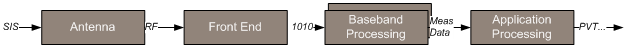
\includegraphics[width=0.7\textwidth]{modelPOR}
	\caption{Funkcionalni model programski određenog radio prijamnika za satelitsku navigaciju}
	\label{Fig:modelPOR}	
\end{figure}

Za područje satelitske navigacije, domena visokih frekvencija izdvojit će i digitalizirati signale koji prenose PRN kodne sekvence i navigacijsku poruku. Nizovi brojeva prosljeđuju se u domenu osnovnog frekvencijskog područja koja identificira i izdvaja prenošene informacije. U satelitskom navigacijskom prijamniku, u ovoj se domeni postupakom unakrsne korelacije primljenih i lokalno generiranih PRN kodnih sekvenci određuju pseudoudaljnosti i izdvajaju elementi navigacijske poruke. U domeni aplikacijskog procesiranja, izlaz osnovnog frekvencijskog područja bit će obrađeni s ciljem predstavljanja (spremanja) informacija u korisniku razumljivom obliku (slika \ref{Fig:modelPOR}).

\section{Pojam programski određenog radioprijamnika}
Tradicionalni prijamnik za satelitsku navigaciju je izveden sklopovski. Elektronički sklopovi posebne namjene obavljaju ciljane funkcije unutar segmenata prijamnika. Pri tome, konstrukcija i izvedba sklopova definira uspješnost primjene matematičkih modela u ispunjavanje traženih funkcionalnosti, odnosno postavljenih zahtjeva na kvalitetu procesiranja signala i informacija.

Elektronički sklopovi su po svojoj su prirodi nesavršeni i ograničeni. Jednom konstruirani i izvedeni elektronički sklopovi posebne namjene ne mogu se lako značajnije promijeniti. Pokaže li se potreba za proširivanjem ili prilagođavanjem novom statusu sustava kao cjeline,
potrebno je napuštanje izvedbe starog sustava i konstrukcija ili kupnja potpuno nove.
U slučaju satelitske navigacije, tradicionalni GPS prijamnik, u kojem je generiranje PRN satelitskih sekvenci izvedeno sklopovskim načinom, uvođenje novih satelita i modernizacija sustava izazivaju napuštanje starog i konstrukciju ili kupnju potpuno novog i kompatibilnog GPS prijamnika.

Dvadesete godine dvadesetog stoljeća uvode novi koncept radiokomunikacijske tehnologije.
Reducira se broj elektroničkih sklopova posebne namjene i uvode programske komponente za obradu signala i informacija. Time se omogućava lakše praćenje promjena sustava i izravnija primjena matematičkih modela u algoritamskom obliku na računalnim podlogama opće namjene, npr. osobna računala ili pametni telefoni.
Novi koncept se naziva programski određen radio (engl. Software-Defined Radio, SDR).
Lakoća prilagodbe promjenama, omogućila je SDR-u da ubrzo postane standard u radiokomunikacijskoj industriji.
Brojni uređaju od pametnih telefona do radijskih i televizijskih prijamnika su izvedeni u obliku SDR-a. Takva izvedba im omogućava postizanje bolje prilagodljivosti, proširivosti, iskorištenja energije i lakše komunikacije s drugim računalnim uređajuma. 

Programska izvedba prijamnika za satelitsku navigaciju zanimljiva je sa stajališta računarne
znanosti. Primjena algoritama za procesiranje signala i informacija podržava raspodjeljivanje
arhitekture sustava. Potpuno procesiranje više ne treba biti u potpunosti izvedeno na jednom uređaju
(npr. pametnom telefonu ili samostalnom GNSS prijamniku) pa se dijelovi postupka obrade prebacuju na druge uređaje. Svaki korišteni uređaj svoj dio obrade obavljaja kvalitetnije i točnije uz jednostavnije
korištenje izvora dodatnih informacija koje mogu pridonijeti poboljšanju točnosti procjene
položaja \cite{ref:46,ref:47}. Navedeni pristup omogućava korištenje računalnog okruženja u
oblaku što dopušta da se prijamniku ostavi samo obrada signala i informacija u frekvencijskoj
domeni. Izlaz obrade signala i informacija u frekvencijskoj domeni pohranjuje se u binarnom obliku
u \textit{RINEX} formatu.

\textit{RINEX}\label{sssec:rinex}
(engl. Receiver Independent Exchange Format) je općeprihvaćena definicija
pohranjivanja izlaza obrade (navigacijskih) satelitskih signala u frekvencijskoj domeni (neobrađeni podatci satelitske navigaciju).
Definiranje općeprihvaćenog načina pohranjivanja omogućava lako prebacivanje dijelova obrade 
na druge uređaje u svrhu poboljšanju točnosti procjene
položaja \cite{ref:46,ref:47}.
\textit{RINEX} se mijenja kroz vrijeme obuhvaćajući promjene GNS sustava. Trenutna verzija je
3.03 iz 2015 \cite{rinex:303}.

\section{Programski određen GPS prijamnik}
Programsko određen GPS prijamnik predstavlja vrstu programski određenog radioprijamnika posebne namjene za procjenu položaja satelitskim navigacijskim sustavima.

Posebnosti programski određenog radioprijamnika za potrebe
satelitske navigacije izražene su karakterističnim postupcima procesiranja signala i informacija u
domeni osnovnog frekvencijskog područja i domeni navigacijskog (aplikacijskog) procesiranja.
Karakteristični postupci su vezani za:
\begin{itemize}
	\item prihvat signala (engl. Acquisition), prepoznavanje PRN kodne sekvence pojedinačnog
	satelitskog signala,
	\item sljeđenje signala (engl. Tracking), vremensko usklađivanje s primljenim signalom, za
	potrebe kasnijeg određivanja pseudoudaljenosti,
	\item procjena vidljivosti satelita,
	\item procjena položaja, brzine i vremena.
\end{itemize}

%PREVESTI SLIKU 
%NAĆI RAZUMLJIVIJU SLIKU
\begin{figure}[H]
	\centering
	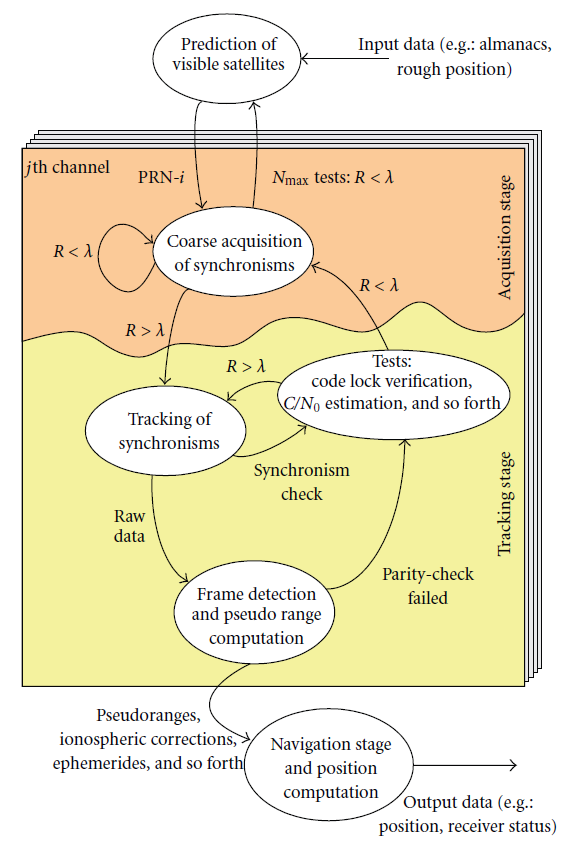
\includegraphics[width=0.7\textwidth]{prihvatSignala}
	\caption{Procesiranje signala u domeni osnovnog frekvencijskog područja}
	\label{Fig:prihvat}	
\end{figure}

Procesiranje signala u domeni osnovnog frekvencijskog područja (slika \ref{Fig:prihvat}) obuhvaća prihvat
signala, sljeđenje signala, izdvajanje navigacijske poruke i određivanje pseudoudaljenosti. Obavlja se
na razini komunikacijskog kanala,tj. za svaki pojedinačni satelitski signal. U slučaju gubitka
vremenske usklađenosti s primljenim signalom, prijamnik će prijeći na prihvat signala, dok se ne
stvore uvjet za ponovni prijelaz u fazu slijeđenja. U slučaju potpunog gubitka signala, prijamnik ponovo započinje postupak prihvata.

Algoritmi obrade signala u domeni osnovnog frekvencijskog područja ovise o spremnosti procjene vidljivosti satelita koja se u navigacijskoj domeni zasniva na pojednostavljenom
opisu satelitskih putanja, efemeridama. Almanah o statusu satelita u sazviježđu, kao i satelitske efemeride, prenosi se navigacijskom porukom. Promjene u almanahu događaju se na
dnevnoj bazi. Ukoliko prijamnik već poznaje dnevni almanah, u stanju je brže napraviti
prvu procjenu položaja, što nazivamo topli start GPS (ili općenito GNSS) prijamnika.
Ukoliko su prijamniku poznati i dnevni almanah i efemeride, vrijeme do prve procjene položaja je još kraće i iznosi nekoliko desetaka sekundi. Nazivamo ga vrućim startom GNSS prijamnika. Ako
prijamnik nema ni dnevni alamanh ni sateliske efemeride, vrijeme do procjene položaja
može biti prilično dugo. Ono ovisi o načinu dobavljanja navigacijske poruke. Ako se poruka
prima sa satelita, vrijeme do prve procjene položaja je barem 12.5 min.Takvo stanje GNSS prijamnika se naziva hladan start GNSS prijamnika. Hladan start je moguće ubrzati alternativnom dostavom navigacijske poruke, npr. preko
telekomunikacijskih mreža. Naime, elementi telekomunikacijskih mreža su vremenski usklađeni pomoću satelitskih
navigacijskih prijamnika pa čvorovi mreže već poznaju navigacijsku poruku i mogu je prenijeti
korisničkoj opremi (GNSS prijamniku). Način rada u kojem
korisnički prijamnik ne prima sve potrebne podatke za određivanje položaja putem satelita nazivamo potpomognutom satelitskom navigacijom (engl. Augmented GNSS, A-GNSS).

Algoritam procesiranja informacija u domeni navigacijske primjene (vidi: poglavlje \ref{sec:algoritam}) koristi informacije iz
navigacijske poruke (satelitske efemeride, alamanah i parametre modela ispravaka pogrešaka) te
izmjerene pseudoudaljenosti kako bi se procijenio položaj (i/ili brzinu) prijamnika i ispravio
pogrešku korisničkog sata. Prvo se modelima ispravaka ispravljaju poznate sustavne pogreške
položaja satelita, ionosferskog i troposferskog kašnjenja te pogreške točnosti \footnote{Ne misli se na preciznost. Pogreške preciznosti korisničkog sata se modeliraju algoritmom procjene položaja uvođenjem četvrte nepoznanice sustava.} korisničkog sata izmjerenih vrijednosti pseudo-udaljenosti. Tako se dobivaju ispravljene mjerene pseudo-udaljenosti  koje se koriste za ulaz algoritma procjene položaja. \\
Slučajne pogreške ostaju nepokrivene pa procjena položaja nije
apsolutno točna. Ipak, postupak procjene položaja omogućuje zadovoljavajuću procjenu pogreške
određivanja položaja. Ona se može predstaviti korisniku, zajedno s rezultatima procjene položaja (i/ili brzine i vremena).\\
Nepokrivenost slučajne pogreške referentnim načinom rada programski određenog radioprijamnika nagnala je mnoge pa i nas na kontrukciju modela redukcije slučajne pogreške (vidi: stranica \pageref{sec:algTezine}). 
Redukcija slučajne pogreške se temelji na modifikaciji referentnog algoritma procjene položaja
za koju postoji mogućnost integracije u izvedeni programski određen radioprijamnik.

\section{Praktična izvedba korisničkog GPS prijamnika}
U okviru diplomskog rada izvaden je korisnički $GPS$ prijamnik.
Izvedeni radioprijamnik je moguće koristiti za obradu satelitskih signala i informacija u domeni osnovnog frekvencijskog područja i domeni navigacijske primjene. Obrada signala u domeni osnovnog frekvencijskog područja se izvodi korištenjem programske knjižnice otvorenog koda \textit{GNSS SDRLIB}
\cite{ref:48}. Obrada informacija u domeni navigacijske primjene je moguće izvesti korištenjem programskog paketa otvorenog koda \textit{RTKNAV} iz programske knjižnice \textit{RTKLIB}\cite{ref:36}.

\begin{figure}[H]
	\centering
	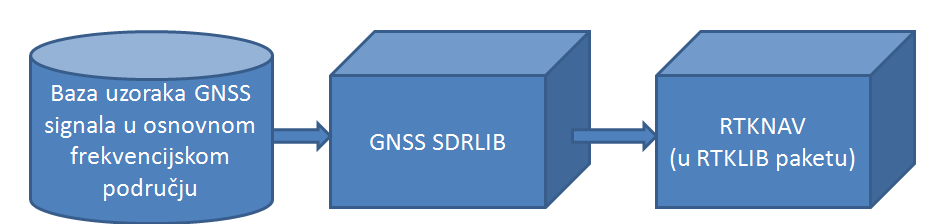
\includegraphics[width=0.7\textwidth]{rtkGNSS}
	\caption{Shema GNSS radioprijamnika}
	\label{Fig:radioprijamnik}	
\end{figure}
Spomenute knižnice povezane su klijentsko-poslužiteljskom arhitekturom.
\vspace{0.5cm}
Programska knjižnica \textit{GNSS SDRLIB} (slika \ref{Fig:sdrlib}) omogućava korištenje kompozitnih
GPS signala (slika \ref{Fig:GPSSignal}) u domeni osnovnog  frekvencijskog područja dostavljenih strujenjem
ili arhivkom datotekom.
Omogućuje izbor pojedinačnog GNSS sustava i pojedinačnih satelita pa tako i odabranog $GPS$ sustava.
Također, omogućava pristup strujanim podatcima potpomognutog GNSS-a,  dostavljanim putem internetske veze od trećih strana (dobavljača ispravaka).
\begin{figure}[H]
	\centering
	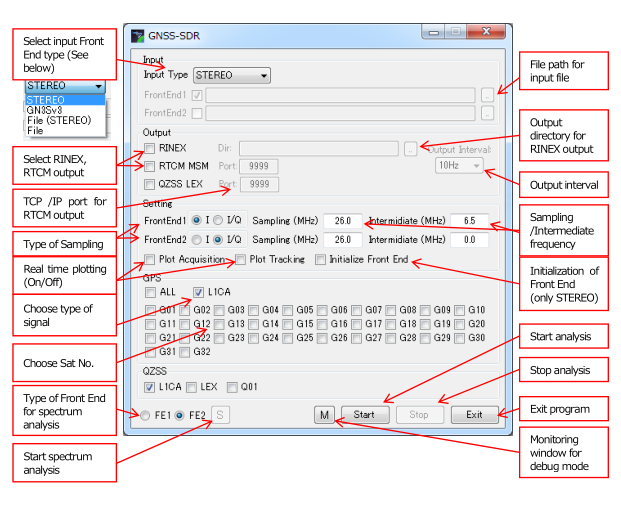
\includegraphics[width=0.8\textwidth]{sdrlib}
	\caption{Grafičko korisničko sučelje programskog paketa GNSS-SDRLIB}
	\label{Fig:sdrlib}	
\end{figure}
%
Programski paket \textit{RTKNAVI} je dio programske knjižnice otvorenog koda \textit{RTKLIB} \cite{ref:36, ref:5}.
Koristi se za procjenu položaja (i/ili brzine i vremena) zasnovanom na podatcima
(pseudoudaljenosti i sadržaja navigacijske poruke) koji čine izlaz domene za obradu signala u osnovnom
frekvencijskom području. Preko grafičkog korisničkog sučelja (Slike \ref{Fig:rtkNav} i \ref{Fig:guirtkNav}) omogućuje
praćenje statusa procesa: toka podataka iz GNSS SDRLIB aplikacije prema RTKNAV aplikaciji,
grafičkog predstavljanja jakosti prihvaćenih i sljeđenih satelitskih signala te procjenu navigacijskih
parametara (tri komponente položaja: geografska širina, geografska dužina i nadmorska visina,
brzina i točno vrijeme) temeljem mjerenih vrijednosti pseudoudaljenosti korištenih
satelita te uz korištenje temeljnog postupka procjene položaja i točnog
vremena (slika \ref{Fig:rtkNavKo}). 
Korišteni algoritmi procesiranja informacija i procjene
položaja opisani su u dokumentraciji programske knjižnice RTKLIB \cite{ref:36}.
\begin{figure}[H]
	\centering
	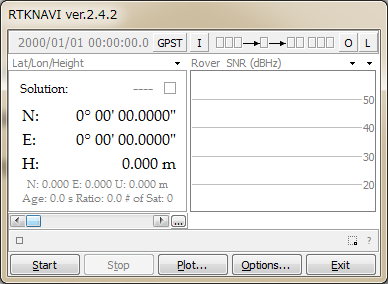
\includegraphics[width=0.6\textwidth]{rtkNav}
	\caption{Grafičkko korisničko sučelje programskog paketa RTKNAV}
	\label{Fig:rtkNav}	
\end{figure}
\begin{figure}[H]
	\centering
	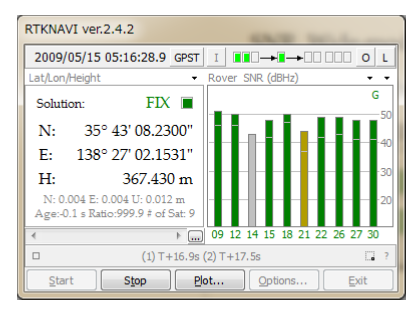
\includegraphics[width=0.6\textwidth]{guirtkNav}
	\caption{GUI RTKNAV aplikacije u radu (zastavica FIX označava ispravnu procjenu položaja)}
	\label{Fig:guirtkNav}	
\end{figure}
\begin{figure}[H]
	\centering
	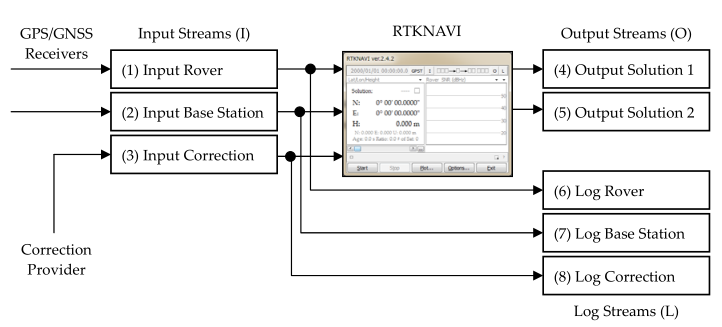
\includegraphics[width=0.8\textwidth]{rtkNavKo}
	\caption{Korištenje aplikacije RTKNAV, s ulaznim i izlaznim informacijama}
	\label{Fig:rtkNavKo}	
\end{figure}

Korišteni uzorci GPS signala u domeni osnovnog frekvencijskog područja\footnote{Spremljeni u RINEX formatu (RINEX podatci).} su pribavljeni eksperimantalno %izvedenim GPS prijamnikom 
u stvarnim uvjetima.
Podešavanjem opcija, izvedeni GPS prijamnik obavlja obradu signala u frekvencijskoj domeni.
Obavlja se i obrada izmjerenih pseudo-udaljenosti referentnim modelima ispravaka.
Potrebni podatci za ulaz 
algoritama procjene položaja u domeni navigacijske primjene su spremljeni u obliku tekstualne datoteke (koordinate satelita i pripadne pseudoudaljenosti). Sadržaj korištenih tekstualnih datoteka dan je u dodatku \ref{appendix:datotekeUlaza} ovoga rada.

%\chapter{Programski jezik R}
%Općenito, $R$ je programski jezik za statističku i drugu matematičku obradbu pomoću računala i ima snažnu grafičku potporu.
%Između ostalog, podržava postupke zasnovane na linearnoj algebri, analizi i prognozi ponašanja vremenskih nizova \cite{ref:34,ref:22}.
%Pogodan je za izvedbu statističke analize, modeliranje i simulacije.\\
%
%\textit{R} je dostupan za većinu korištenih platformi (Microsoft Windows, Linux, Mac OS X), a instalacija je poprilično jednostavna.
%Potrebno je samo preuzeti potrebne datoteke s web-stranice \cite{Rsite} i u skladu s njima instalirati program.
%Instalirani program nudi R-sučelje (R-GUI) u kojemu se preko naredbene linije zadaju naredbe i pokreću skripte, a dobivaju numerički i grafički rezultati.
%Postoji i više neslužbenih R-sučelja. Jedan od poznatijih je \textit{R-Studio} \cite{RStudio}.
%Ovdje se komunikacija opet ostvaruje preko naredbi u konzoli, ali je RStudio opremljen znantno bogatijom grafičkom okolinom (radni prostor, povijest, instalacija paketa, pomoć i sl.).
%Postoji i mogućnost integracije $R$ interpretera u odabrani tekst-editor ili poziva R-funkcija iz drugih programskih jezika (Python, Ruby, SAGE).
%\\
%ZA KNJIGU OVO GORE POGLAVLJE NADOPUNITI

\chapter{Praktična izvedba procjene položaja u domeni navigacijske primjene}\label{sec:izvedba}
Prije korištenja algoritma za procjene položaja, u domeni navigacijske primjene,
obavljaju se sljedeće radnje (procesiranje informacija u domeni navigacijske primjene):
\begin{enumerate}
	\item Prikupljaju se potrebni podatci izlaza domene osnovnog frekvencijskog područja: (1) djelovi navigacijske poruke (satelitske efemeride, dnevni almanah i parametri modela ispravaka) i (2) mjerene pseudo-udaljenosti,
	\item Ispravljaju se mjerene psudo-udaljenosti prikupljenim podatcima modelima ispravaka.
\end{enumerate}
Za potrebe ovoga rada, gornje radnje su obavljene primjereno podešen koristeći izvedeni programski određen radioprijamnik. 
Izlaz gornjih radnji su dvije datoteke ulaza algoritma procjene položaja: (1) datoteka 
ispravljenih pseud-oudaljenosti i (2) datoteka satelitskih efemerida pripadnih satelita.
Primjer njihovog sadržaja je dan u dodatku \ref{appendix:datotekeUlaza}.\\
Općenito, gornje radnje mogu biti izrazito kompleksne i prelaze obujam ovoga rada.\\
U praksi korišteni algoritmi procjene položaja u domeni navigacijske primjene opisani su dokumentacijom programske knjižnice RTKLIB \cite{ref:36}. \\
Ovo poglavlje najprije opisuje dva načina linearizacije nelinearnog sustava jednadžbi iz poglavlja \ref{sec:positionProcess},a zatim numeričke metode koje je moguće iskoristiti u rješavanju lineariziranog sustava jednadžbi iterativnog postupka. Na kraju su opisana dva pristupa izvedbi procjene položaja u domeni navigacijske primjene.
\vspace{0.2cm}

\subsection{Prvi način linearizacije jednadžbi sustava}
Prvi način linearizacije jednadžbi sustava dobivamo promatrajući sustav \ref{eq:1} s $v_i = p_i$(\textbf{x}):
\begin{align}\label{eq:1partial}
d_1 = \sqrt{(x-x_1)^{2}+(y-y_1)^{2}+(z-z_1)^{2}} + c\cdot d_T + p_1(\mathbf{x})\notag \\
d_2 = \sqrt{(x-x_2)^{2}+(y-y_2)^{2}+(z-z_2)^{2}} + c\cdot d_T + p_2(\mathbf{x})\\
d_3 = \sqrt{(x-x_3)^{2}+(y-y_3)^{2}+(z-z_3)^{2}} + c\cdot d_T + p_3(\mathbf{x}) \notag \\
d_4 = \sqrt{(x-x_4)^{2}+(y-y_4)^{2}+(z-z_4)^{2}} + c\cdot d_T + p_4(\mathbf{x}) \notag
\end{align}
u $\mathbf{x} = (x,y,z,d_T)$.\\
Sada je:
\begin{align}
p_i(\mathbf{x}) = \sqrt{(x-x_1)^{2}+(y-y_1)^{2}+(z-z_1)^{2}} + c\cdot d_T- d_i
\end{align}
Linearizacijom jednadžbi sustava (\ref{eq:1partial}) na način korišten na stranici \pageref{stranica:NGLin} (za Newton-Gaussovu metodu), dobivamo:
\begin{align}
p_i(\mathbf{x} + \Delta\mathbf{x}) = p_i(\mathbf{x}) + \frac{\partial p}{\partial x}\Delta x + \frac{\partial p}{\partial y}\Delta y + \frac{\partial p}{\partial z}\Delta z + \frac{\partial p}{\partial d_T}\Delta d_T 
\end{align}
Koristeći iterativni postupak, svaki korak $k$ definira $\mathbf{x}_{k+1} = \mathbf{x}_k+\Delta\mathbf{x}_k$
gdje je $\Delta \mathbf{x}_{k}$ rješenje sustava $k$-tog koraka. Nastoji se postići $\mathbf{p}(\mathbf{x}_k+\Delta\mathbf{x}_{k+1}) = 0$
%Budući da se $(d_1,d_2,d_3,d_4)$ ne mijenjaju kroz iteracije, dobivamo izraz:
%$$
%d_i = f_i(\mathbf{x}_{k+1}) = f_i(\mathbf{x}_{k} + \Delta\mathbf{x}_{k}) = f_i(\mathbf{x}_{k}) + %\frac{\partial f}{\partial x}\Delta x_k + \frac{\partial f}{\partial y}\Delta y_k + \frac{\partial %f}{\partial z}\Delta z_k + \frac{\partial f}{\partial d_T}\Delta (d_T)_k $$
što daje
\begin{align}
p_i(\mathbf{x}_{k}) + \frac{\partial p_i}{\partial x}\Delta x_k + \frac{\partial p_i}{\partial y}\Delta y_k + \frac{\partial p_i}{\partial z}\Delta z_k + \frac{\partial p_i}{\partial d_T}\Delta (d_T)_k = 0,
\end{align}
odnosno
\begin{align}
- p_i(\mathbf{x}_{k}) &= d_i - \sqrt{(x_k-x_i)^{2}+(y_k-y_i)^{2}+(z_k-z_i)^{2}} - c\cdot (d_T)_k = \notag \\
\frac{\partial f}{\partial x}\Delta x_k + \frac{\partial f}{\partial y}\Delta y_k + \frac{\partial f}{\partial z}\Delta z_k + \frac{\partial f}{\partial d_T}\Delta (d_T)_k &= 
\begin{bmatrix}
\frac{\partial f_i}{\partial x} &
\frac{\partial f_i}{\partial y} &
\frac{\partial f_i}{\partial z} &
\frac{\partial f_i}{\partial d_T}
\end{bmatrix}
\begin{bmatrix}
\Delta x \\
\Delta y \\
\Delta z \\
\Delta d_T
\end{bmatrix}  
\end{align}
Uz 
\begin{align}\label{eq:definicijaSustava1}
\mathbf{A} & := \begin{bmatrix}
\frac{\partial p_1}{\partial x} &
\frac{\partial p_1}{\partial y} &
\frac{\partial p_1}{\partial z} &
\frac{\partial p_1}{\partial d_T} \\
\frac{\partial p_2}{\partial x} &
\frac{\partial p_2}{\partial y} &
\frac{\partial p_2}{\partial z} &
\frac{\partial p_2}{\partial d_T} \\
\frac{\partial p_3}{\partial x} &
\frac{\partial p_3}{\partial y} &
\frac{\partial p_3}{\partial z} &
\frac{\partial p_3}{\partial d_T} \\
\frac{\partial p_4}{\partial x} &
\frac{\partial p_4}{\partial y} &
\frac{\partial p_4}{\partial z} &
\frac{\partial p_4}{\partial d_T}
\end{bmatrix} \\
& = \begin{bmatrix}
\frac{(x-x_1)}{\sqrt{(x-x_1)^{2}+(y-y_1)^{2}+(z-z_1)^{2}}} & \frac{(y-y_1)}{\sqrt{(x-x_1)^{2}+(y-y_1)^{2}+(z-z_1)^{2}}} & \frac{(z-z_1)}{\sqrt{(x-x_1)^{2}+(y-y_1)^{2}+(z-z_1)^{2}}} & c \\
\frac{(x-x_2)}{\sqrt{(x-x_2)^{2}+(y-y_2)^{2}+(z-z_2)^{2}}} & \frac{(y-y_2)}{\sqrt{(x-x_2)^{2}+(y-y_2)^{2}+(z-z_2)^{2}}} & \frac{(z-z_2)}{\sqrt{(x-x_2)^{2}+(y-y_2)^{2}+(z-z_2)^{2}}} & c \\
\frac{(x-x_3)}{\sqrt{(x-x_3)^{2}+(y-y_3)^{2}+(z-z_3)^{2}}} & \frac{(y-y_3)}{\sqrt{(x-x_3)^{2}+(y-y_3)^{2}+(z-z_3)^{2}}} & \frac{(z-z_3)}{\sqrt{(x-x_3)^{2}+(y-y_3)^{2}+(z-z_3)^{2}}} & c \\
\frac{(x-x_4)}{\sqrt{(x-x_4)^{2}+(y-y_4)^{2}+(z-z_4)^{2}}} & \frac{(y-y_4)}{\sqrt{(x-x_4)^{2}+(y-y_4)^{2}+(z-z_4)^{2}}} & \frac{(z-z_4)}{\sqrt{(x-x_4)^{2}+(y-y_4)^{2}+(z-z_4)^{2}}} & c \\
\end{bmatrix} \notag \\
\mathbf{x} & :=  \begin{bmatrix}
\Delta x \\
\Delta y \\
\Delta z \\
\Delta d_T
\end{bmatrix} \\
\mathbf{b} & := \begin{bmatrix}
d_1 - \sqrt{(x_k-x_1)^{2}+(y_k-y_1)^{2}+(z_k-z_1)^{2}} - c\cdot (d_T)_k \\
d_2 - \sqrt{(x_k-x_2)^{2}+(y_k-y_2)^{2}+(z_k-z_2)^{2}} - c\cdot (d_T)_k \\
d_3 - \sqrt{(x_k-x_3)^{2}+(y_k-y_3)^{2}+(z_k-z_3)^{2}} - c\cdot (d_T)_k \\
d_4 - \sqrt{(x_k-x_4)^{2}+(y_k-y_4)^{2}+(z_k-z_4)^{2}} - c\cdot (d_T)_k
\end{bmatrix}
\end{align}%ISTO DEFF NA STR 41 http://www2.imm.dtu.dk/pubdb/views/edoc_download.php/2804/pdf/imm2804.pdf
dobivamo sustav
\begin{align}\label{eq:sustav}
\mathbf{A}\mathbf{x} = \mathbf{b}
\end{align}
koji rješavamo metodom iterativnih najmanjih kvadrata.\label{stranica:nastavakLS}

\subsection{Drugi način linearizacije jednadžbi sustava}
Drugi način linearizacije se dobiva promatrajući isti sustav jednadžbi (\ref{eq:1}).
Metoda iterativnih najmanjih kvadrata se ne primjenjuje izvorno na početni sustav, već na njegovu modifikaciju, modifikaciju sustava \ref{eq:new}.
Modificirani sustav je u mogućnosti dati isto dobro rješenje uz uvjet $cd_T < d_i, \forall i \in \{1,2,3,4\}$. \\

Prebacujući član $d=d_T \cdot c$ na lijevu stranu i kvadrirajući obje strane
jednadžbi sustava (\ref{eq:new}) dobivamo modificirani sustav jednadžbi:
\begin{align}\label{eq:newIzvedba}
(d_1-d)^2 = (x-x_1)^{2}+(y-y_1)^{2}+(z-z_1)^{2} + p_1(\textbf{x})\notag \\
(d_2-d)^2 = (x-x_2)^{2}+(y-y_2)^{2}+(z-z_2)^{2} + p_2(\textbf{x})\\
(d_3-d)^2 = (x-x_3)^{2}+(y-y_3)^{2}+(z-z_3)^{2} + p_3(\textbf{x})\notag \\
(d_4-d)^2 = (x-x_4)^{2}+(y-y_4)^{2}+(z-z_4)^{2} + p_4(\textbf{x})\notag
\end{align}
gdje je 
\begin{align}
p_i(\textbf{x}) & = 2\sqrt{(x-x_i)^{2}+(y-y_i)^{2}+(z-z_i)^{2}}v_i + v_i^2.
\end{align} i
\begin{align}
p_i(\textbf{x}) & = (d_i-d)^2 - (x_i-x)^{2} - (y_i-y)^{2} - (z_i-z)^{2}.
\end{align}
Označimo 
\begin{align} \mathbf{\tilde{p}}(\mathbf{x}) := (p_1(\textbf{x}),p_2(\textbf{x}),p_3(\textbf{x}),p_4(\textbf{x}))^T
\end{align}
pa problem minimizacije \ref{eq:minimization} prelazi u
\begin{align}\label{eq:minimisation3}
\hat{\mathbf{x}} = \text{arg min}_\mathbf{x} \mathbf{\tilde{p}}(\mathbf{x})^T\mathbf{\tilde{p}}(\mathbf{x}).
\end{align}
i $$ \mathbf{\tilde{p}'}(\mathbf{x}) = (p_1'(\textbf{x}),p_2'(\textbf{x}),p_3'(\textbf{x}),p_4'(\textbf{x}))^T 
= \begin{bmatrix}
2(x_1-x) &  2(y_1-y) &  2(z_1-z) & - 2c(d_1-cd_T)\\
2(x_2-x) &  2(y_2-y) &  2(z_2-z) & - 2c(d_2-cd_T) \\
2(x_3-x) &  2(y_3-y) &  2(z_3-z) & - 2c(d_3-cd_T) \\
2(x_4-x) &  2(y_4-y) &  2(z_4-z) & - 2c(d_4-cd_T) 
\end{bmatrix}
.$$
\\Neka je
\begin{align}
& \mathbf{P} := \begin{bmatrix}
(x_1-x) & (y_1-y) & (z_1-z) & (d_1-d) \\
(x_2-x) & (y_2-y) & (z_2-z) & (d_2-d) \\
(x_3-x) & (y_3-y) & (z_3-z) & (d_3-d) \\
(x_4-x) & (y_4-y) & (z_4-z) & (d_4-d) 
\end{bmatrix} \\
& \tilde{\mathbf{I}} := diag(1,1,1,-c) \\
& \mathbf{\tilde{\mathbf{P}'}}:= 2 \mathbf{P}\tilde{\mathbf{I}} .
\end{align}
Imamo 
\begin{align}
\Delta \mathbf{x_k} = -(2 \mathbf{P}\tilde{I} )^{-1}(\mathbf{\tilde{p}}(\mathbf{x_k}))
\\= -\frac{1}{2}(\mathbf{P}\tilde{\mathbf{I}} )^{-1}(\mathbf{\tilde{p}}(\mathbf{x_k})).
\end{align}

Uz oznake  
\begin{align}\label{eq:deffDrugaFakt}
\mathbf{A} := \mathbf{\tilde{P'}} \notag\\
\mathbf{b} := - \mathbf{\tilde{p}}(\mathbf{x_k})
\end{align}
svaka iteracija algoritma \ref{algorithm:iterLSM} sa stranice \pageref{algorithm:iterLSM},
računa $\Delta \mathbf{x_k}$ rješavajući sustav
\begin{align}\label{eq:drugaFakt}
\mathbf{A} \mathbf{x} = \mathbf{b}
\end{align}
u $\mathbf{x}:= \Delta \mathbf{x_k}$.
\vspace{0.5cm}
\\Analogno, \ref{eq:minimisation2} prelazi u 
\begin{align}\label{eq:minimisation4}
\hat{\mathbf{x}} = \text{arg min}_\mathbf{x} \mathbf{\tilde{p}}(\mathbf{x})^T \Sigma ^{-1}\mathbf{\tilde{p}}(\mathbf{x}).
\end{align}
i uz  
\begin{align}
\mathbf{A} := \Sigma^{-\frac{1}{2}}\mathbf{\tilde{P'}} \notag\\
\mathbf{b} := - \Sigma^{-\frac{1}{2}} \mathbf{\tilde{p}}(\mathbf{x_k}) \notag \\
\end{align}
svaka iteracija algoritma \ref{algorithm:iterLSMW} rješava sustav \ref{eq:drugaFakt}.

\subsection{Numerička linearna algebra za rješavanje dobivenog (lineariziranog) sustava problema najmanjih kvadrata}
Pogreške u mjerenjima ili linearizacija uvjetuju da sustav \ref{eq:sustav} nema uvijek rješenje, tj. 
$\mathbf{A}\mathbf{x} - \mathbf{b} \not = 0, \forall \mathbf{x} \in \R^m$. 
Zato ideja rješavanja sustava problema najmanjih kvadrata nije tražiti rješenje sustava, već $\mathbf{x}$ koji minimizira izraz $\|\mathbf{A}\mathbf{x} - \mathbf{b}\|_2$. \\

Neki od najbitnijih koncepta za pronalazak rješenja sustava u smislu najmanjih kvadrata jesu \cite{svd_QR_normalEquations}: 
\begin{itemize}
	\item sustav normalnih jednadžbi,
	\item QR dekompozicija,
	\item SVD,
\end{itemize}
a objašnjeni su u nastavku.

\subsubsection{Sustav normalnih jednadžbi}
Sustavi normalnih jednadžbi su značajni za rješavanje problema najmanjih kvadrata jer se njihovim rješavanjem 
dobiva rješenje jednako rješenju pripadnog problema najmanjih kvadrata. \\
Dakle, za pronalazak rješenja sustava:
\begin{align}
\mathbf{A}\mathbf{x} = \mathbf{b}
\end{align}
u smislu najmanjih kvadrata je dovoljno promatrati pripadni sustav (normalnih jednadžbi):
\begin{align}
\mathbf{A}^T\mathbf{A}\mathbf{x} = \mathbf{A}^Tb.
\end{align}
Dokaz je dan teoremom \ref{thm:1}.

\begin{thm}\label{thm:1}
	Skup svih rješenja problema $\min_\mathbf{x}\| \mathbf{A}\mathbf{x} - \mathbf{b} \|_2$ označimo s
	$$ S= \{\mathbf{x} \in \R^\mathit{m} | \| \mathbf{A}\mathbf{x} - \mathbf{b} \|_2 \textit{ je minimalna} \} $$
	Tada je $\mathbf{x}  \in S$, tj. $\mathbf{x}$ je rješenje problema najmanjih kvadrata, ako i samo ako vrijedi sljedeća relacija ortogonalnosti 
	$$\mathbf{A}^T(\mathbf{A}\mathbf{x}-\mathbf{b}) = 0,$$
	\\ koju obično nazivamo \textit{sustav normalnih jednadžbi} i pišemo u obliku 
	$$ \mathbf{A}^T\mathbf{A}\mathbf{x} = \mathbf{A}^Tb $$.
	\end{thm}
	\begin{proof}
		Rješavanje problema $\mathbf{A}\mathbf{x} = \mathbf{b}$, gdje $\mathbf{x}$ parametar koji je potrebno odrediti, se svodi na prikaz vektora $\mathbf{b}$ u bazi koju čine stupci matrice $\mathbf{A}$. Ukoliko $\mathbf{b}$ nije iz prostora razapetog stupcima matrice $\mathbf{A}$, $L_A$,
		tada je potrebno pronaći vektor $\mathbf{\hat{b}} \in L_A$ i
		najbliži vektoru $\mathbf{b}$ među svim vektorima iz $L_A$.
		Po definiciji, $\mathbf{\hat{b}}$ je projekcija $\mathbf{b}$ na $L_A$ dana formulom:
		\begin{align*}
		\mathbf{\hat{b}} := \mathbf{A(A^TA)^{-1}A^T}\mathbf{b}
		\end{align*}
		\begin{figure}[H]
			\centering
			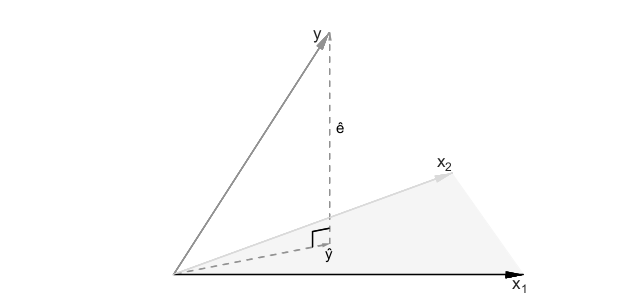
\includegraphics[width=0.8\textwidth]{linProjection}
			\caption{Projekcija vektora $\mathbf{y}$ u prostor razapet vektorima $x_1$ i $x_2$ \cite{svd_str15} }
			\label{Fig:projection}	
			\end{figure}
			
			Izraz $\mathbf{A(A^TA)^{-1}A^T}$ nazivamo projektor na prostor razapet stupcima matrice $\mathbf{A}$ i obično se označava s $\mathbf{H}$.\\
			Vrijedi da je $\mathbf{\hat{x}}$ rješenje problema najmanjih kvadrata ako i samo ako
			vrijedi $\mathbf{A}\mathbf{\hat{x}} = \mathbf{\hat{b}}$, tj.
			$\mathbf{\hat{x}}:= \mathbf{(A^TA)^{-1}A^T}\mathbf{b}$\label{eq:lin1Xeq}. Zaključujemo kako je $\mathbf{\hat{x}}$ rješenje problema najmanjih kvadrata ako i samo ako je $\mathbf{\hat{x}}$ \textbf{rješenje problema normalnih jednadžbi}
			\begin{align}\label{eq:sustavProj}
			\mathbf{A}^T\mathbf{A}\mathbf{x} = \mathbf{A}^T\mathbf{b}.
			\end{align}
			\end{proof}
Detaljniji dokaz teorema se može pronaći u \cite{singer07} na stranici 46.\\

Napomenimo da spomenuti sustav normalnih jednadžbi ima i sljedeća svojstva:%
\begin{enumerate}
	\item Općenito, matrica $\mathbf{A}^T\mathbf{A}$ je simetrična i pozitivno semidefinitna jer za svaki
	$\mathbf{x} \in \R^m$ vrijedi
	\begin{align}
	\mathbf{x}^T\mathbf{A}^T\mathbf{A}\mathbf{x} = (\mathbf{A}\mathbf{x})^T(\mathbf{A}\mathbf{x}) = \|A\mathbf{x}\|_2^2 \geq 0.
	\end{align}
		\item Sustav normalnih jednadžbi uvijek ima rješenje i to jedinstveno.
\end{enumerate}
koja olakšavaju njegovo rješavanje.
\vspace{1cm}

Nakon konačne formalizacije problema, potrebno je izabrati način izračunavanja rješenja sustava \eqref{eq:sustavProj}.
Obično se matrica $\mathbf{A}^T\mathbf{A}$ ne invertira, nego se rješava sustav \eqref{eq:sustavProj}.

Sustav se obično rješava koristeći dekompoziciju Choleskoga matrice $\mathbf{A}^T\mathbf{A}$.
Tako pronađeno rješenje obično nije zadovoljavajuće točnosti (vidi: \cite{singer07}, stranica 60).

\subsubsection{QR dekompozicija}\label{sec:QR}
Pristup rješavanja problema najmanjih kvadrata $QR$ dekompozicijom zasniva se na činjenici da je matrica sustava punog stupčanog ranga pa rješenje opisuje na sljedeći način
\begin{align}\label{eq:useQR}
\min_{\mathbf{x}} \| \mathbf{A}\mathbf{x} - \mathbf{b} \|_2	
& = \min_{\mathbf{x}} \| \mathbf{Q}^T(\mathbf{A}\mathbf{x} - \mathbf{b}) \|_2 \\
& =  \min_{\mathbf{x}}\| \mathbf{Q}^T \mathbf{A}\mathbf{x} - \mathbf{Q}^T \mathbf{b} \|_2	\notag
\end{align}
gdje je $\mathbf{Q}$ proizvoljna ortogonalna matrica.\\
Kako $\mathbf{Q}$ može biti proizvoljna, može se odabrati $\mathbf{Q}$ takva da pojednostavljuje izračun za $\mathbf{x}$.
Ukoliko se koristi $\mathbf{Q}$ iz \textit{QR} dekompozicije matrice $\mathbf{A}$ imamo $\mathbf{A} = \mathbf{QR}$, $\mathbf{Q}^T\mathbf{A} = \mathbf{R}$ i $\mathbf{R}$ je gornjetrokutasta matrica.
Dalje se rješava sustav
\begin{align}\label{eq:sustavQR}
\mathbf{R}\mathbf{x} = \mathbf{Q}^T\mathbf{b}.
\end{align}
tj. traži se  
\begin{align}
\mathbf{x} & = \mathbf{R}^{-1}\mathbf{Q}^T\mathbf{b} \notag \\
& = \mathbf{R}^{-1}\mathbf{R}^{-T}\mathbf{R}^{T}\mathbf{Q}^T\mathbf{b} \notag \\
& = (\mathbf{R}^{T}\mathbf{R})^{-1}(\mathbf{QR})^{T}\mathbf{b} \\
& = (\mathbf{R}^{T} \mathbf{I} \mathbf{R})^{-1}(\mathbf{QR})^{T}\mathbf{b}  \notag \\
& = (\mathbf{R}^{T} \mathbf{Q}^T\mathbf{Q} \mathbf{R})^{-1}(\mathbf{A})^{T}\mathbf{b} \notag \\
& = (\mathbf{A}^{T}\mathbf{A})^{-1}(\mathbf{A})^{T}\mathbf{b}.\notag 
\end{align}
Gledajući gornju jednakost odozdo prema gore opažamo kako je rješenje sustava normalnih jednadžbi jednako rješenju trokutastog sustava početnog sustava jednadžbi \ref{eq:sustavQR}.\\
Dakle, dobiveno rješenje također je jednako rješenju problema najmanjih kvadrata dobivenog sustava jednadžbi.
%Jednakost daje i da će rješenje uvijek postojati.

%\textit{QR} dekompozicija se analogno primjenjuje i na sustav nominalnih jednadžbi. %rješava se automatski u R-u
%Kada to ne bi bio slučaj, moglo bi se dogoditi da sustav nema rješenja. Naime, prije primjene metode najmanjih kvadrata za pronalazak rješenja, linearizira se početni sustav jednadžbi i uvode se pogreške.
Rješenje sustava \eqref{eq:sustavQR} se također pronalazi kao rješenje pripadnog problema najmanjih kvadrata. Kako je matrica sustava
gornjetrokutasta, novi sustav je znatno jednostavnije riješiti.
Rješenje dobiveno koristeći \textit{QR} dekompoziciju je stabilnije i ostvaruje manje odstupanje nego rješenje dobiveno
direktnim izračunom $\mathbf{\hat{x}}:= \mathbf{(A^TA)^{-1}A^T}\mathbf{b}$ ili korištenjem dekompozicije Choleskoga matrice $\mathbf{A^TA}$.\\
Općenito, \textit{QR} dekompoziciju možemo koristi i prilikom direktnog računa 
inverza općenite matrice \textbf{A}:
\begin{align}
\mathbf{A}^{-1} = \mathbf{R}^{-1}\mathbf{Q}^{-1} = \mathbf{R}^{-1}\mathbf{Q^T}.
\end{align}
Posebno svojstvo matrice \textbf{R} rezultira jednostavnijem i stabilnijem izračunavanjem inverza matrice \textbf{A}.

\subsubsection{SVD dekompozicija}
\begin{defn}[SVD dekompozicija matrice]
	Neka je \textbf{A} $\in \R^{m\times n}$ ili $\C^{m \times n}$, $SVD$ dekompozicija (engl. Singular Value Decompozition) matrice je $\mathbf{A} = \mathbf{UDV}^*$, $\mathbf{U} \in \R^{m\times m}$ ili $\C^{m\times m}$ unitarna matrica, $\mathbf{V} \in \R^{n\times n}$ ili $\C^{n\times n}$ unitarna matrica i $\mathbf{D} \in \R^{m\times n}$ nenegativna dijagonalna matrica. \\
	Nadalje, stupci matrice \textbf{U} su svojstveni vektori matrice $\mathbf{MM}^*$, dok su stupci matrice \textbf{V} 
	svojstveni vektori matrice $\mathbf{M}^*\mathbf{M}$. Dijagonalni elementi matrice $\mathbf{D}$ su korijeni svojstvenih vrijednosti matrice $\mathbf{M}^*\mathbf{M}$ ili $\mathbf{MM}^*$.
\end{defn}%

Prva primjena \textbf{SVD} dekompozicije je u računu inverza proizvoljne matrice \textbf{A}:%
\begin{align}
\mathbf{A}^{-1} := \mathbf{V}^{-*}\mathbf{D}^{-1}\mathbf{U}^{-1} := \mathbf{V}\mathbf{D}^{-1}\mathbf{U}^*
\end{align}
Kako su za izračun inverza sada potrebni samo inverz dijagonalne matrice i hermitski adjugirana matrica proizvoljne matrice, \textbf{SVD} dekompozicija znatno olakšava izračun inverza.
 

Nadalje, \textit{SVD} dekompozicija se koristi i prilikom rješavanja sustava linearnih jednadžbi.\\
Kako su u sklopu ovoga rada definirani samo sustavi realnih matrica sustava, može se pretpostaviti kako
za \textbf{U},\textbf{D} i \textbf{V} matrice \textbf{SVD} dekompozicije matrice \textbf{A}
vrijedi $\mathbf{U}^* = \mathbf{U}^T$, $\mathbf{D}^* = \mathbf{D}^T = \mathbf{D}$, $\mathbf{V}^* = \mathbf{V}^T$ i \textbf{U} i \textbf{V} su ortogonalne matrice.
Sada se za \textbf{Q} iz \eqref{eq:useQR} može uzeti da je jednaka matrici \textbf{U}. 

Dobiva se sljedeće:
\begin{align}\label{eq:useSVD}
\| \mathbf{A}\mathbf{x} - \mathbf{b} \|_2	
& = \| \mathbf{U}^T(\mathbf{A}\mathbf{x} - \mathbf{b}) \|_2 \\
& = \| \mathbf{U}^T \mathbf{A}\mathbf{x} - \mathbf{U}^T \mathbf{b} \|_2	\notag \\
& = \| \mathbf{D} \mathbf{V}^T\mathbf{x} - \mathbf{U}^T \mathbf{b} \|_2 \notag
\end{align}
Dalje se onda rješava sustav nominalnih jednadžbi
\begin{align}
(\mathbf{D} \mathbf{V}^T)^T\mathbf{D} \mathbf{V}^T\mathbf{x} 
& = (\mathbf{D} \mathbf{V}^T)^T\mathbf{U}^T \mathbf{b} \notag \\
\end{align} i rješenje za \textbf{x} je jednako
\begin{align}
\mathbf{x} = \mathbf{V}\mathbf{D}^{-1}\mathbf{U}^T \mathbf{b}.
\end{align}
Primjer rješavanja problema opisanog sustavom $\mathbf{A}\mathbf{x} = \mathbf{b}$ koristeći SVD dekompoziciju u programskom okruženju $R$ dano je izvorom \cite{svd_Rexample}.
\label{page:boljaQRzaSustav}%OBJ ZASTO BOLJE QR an ne svd u rj sustava


\newpage
Problemi najmanjih kvadrata definirani ovim radom opisani su zasićenim ili prezasićenim sustavima jednadžbi za čije se rješavanja potiče korištenje \textit{QR} dekompozicije \cite{svd_str15}.\\
Pristup rješavanja problema najmanjih kvadrata koji koristi sustav normalnih jednadžbi dekompozicijom Choleskoga se smatra najbržim, ali najmanje stabilnim. Dekompoziciju Choleskoga nije moguće izračunati već ukoliko je uvjetovanost matrice početnog sustava blizu $\frac{1}{\sqrt{\text{strojna točnost}}}$. Pristup koji koristi $QR$ dekompoziciju povećava broj korištenih operacije pa i vrijeme rješavanja problema, ali je stabilniji. Nije ga moguće koristiti tek kada je uvjetovanost matrice blizu  $\frac{1}{\text{strojna točnost}}$. Ono postiže najbolju relativnu pogrešku u smislu najmanjeg kvadratnog odstupanja \cite{svd_QR_normalEquations_comparison_str42}.
SVD pristup je najstabilniji, ali najsporiji. Za razliku od ostalih, jednakom težinom pronalazi i rješenje 
nezasićenog sustava jednadžbi.\\

%Trade off stabilnosti i vremena potrebnog za njezino provođenje.
%Ch , QR , SVD od najbže ka sporijima
%i SVD, QR, Ch stabilnost 
%i QR postiže  


Zanimljivo je da uz poznato
jedno rješenje sustava \ref{eq:sustavProj}, relativno lagano je pronaći i sva ostala.\\
Naime, uz $\mathbf{A}\mathbf{x} - \mathbf{b} = \mathbf{r}$ i proizvoljan $\hat{\mathbf{x}} \in \R^m$ za koji vrijedi
\begin{align}
\hat{\mathbf{r}}  &=  \mathbf{A}\mathbf{\hat{x}} - \mathbf{b} \notag \\
&= \mathbf{A}\mathbf{\hat{x}} + \mathbf{r} - \mathbf{A}\mathbf{x} \\
&= \mathbf{r} + \mathbf{A}(\mathbf{\hat{x}} - \mathbf{x}) \notag
\end{align}
imamo da je $\mathbf{\hat{x}} \in S$ ako i samo ako $\hat{\mathbf{r}} = \mathbf{r}$, tj.  $ \mathbf{A}(\mathbf{\hat{x}} - \mathbf{x}) = 0$ i $\mathbf{\hat{x}} - \mathbf{x} \in \mathcal{N}(\mathbf{A})$.\\
Također, ukoliko je ispunjen jedan od sljedećih uvjeta:%
\begin{itemize}
	\item $\mathbf{A}$ ima puni stupčani rang,
	\item stupci matrice $A$ su linearno nezavisni,
	\item $\mathbf{A}^T\mathbf{A}$ je pozitivno definitna,
\end{itemize}
$\mathcal{N}(\mathbf{A})$ je trivijalan i rješenje sustava je jedinstveno. 
\vspace{0.2cm}

\section{Izvedbe}

Opisuju se dva pristupa izvedbi procesa procjene položaja.
Prvo pristup je osnovni pristup i obuhvaća izvedbe osnovnog (referentnog) algoritma. Drugi pristup je poboljšani pristup i predstavlja predložak  poboljšanja osnovnog pristupa poboljšanjem osnovnog algoritma.
Osnovni algoritam predstavlja algoritam najmanjih kvadrata ( algoritam \ref{algorithm:iterLSM}, stranica \pageref{algorithm:iterLSM}).
Poboljšanje osnovnog algoritma ostvaruje se uvođenjem težina, odnosno upotrebom algoritma \ref{algorithm:iterLSMW} sa stranice \pageref{algorithm:iterLSMW}.
Oba algoritma za dobivene psudoudaljenosti i 
položaj satelita u ECEF XYZ koordinatnom sustavu algoritmi izračunavaju položaj
prijamnika i pogrešku sata prijamnika.\\ 

Izvedba algoritama je ostvarena korištenjem programskog jezika $R$ \cite{ref:24} i R-sučelja \textit{RStudio} na GNU/Linux operativnom sustavu.
Općenito, $R$ je programski jezik za statističku i drugu matematičku obradbu pomoću računala i ima snažnu grafičku potporu.
Između ostalog, podržava postupke zasnovane na linearnoj algebri, analizi i prognozi ponašanja vremenskih nizova \cite{ref:22}.
Pogodan je za izvedbu statističke analize, modeliranje i simulacije.

\textit{R} je dostupan za većinu korištenih platformi (Microsoft Windows, Linux, Mac OS X), a instalacija je poprilično jednostavna.
Potrebno je samo preuzeti potrebne datoteke s web-stranice \cite{Rsite} i u skladu s njima instalirati program.
Instalirani program nudi grafičko-korisničko R-sučelje (R-GUI) u kojemu se preko naredbene linije zadaju naredbe i pokreću skripte, a dobivaju numerički i grafički rezultati.
Postoji i više neslužbenih R-sučelja. Jedan od poznatijih je \textit{R-Studio} \cite{RStudio}.
Ovdje se komunikacija opet ostvaruje preko naredbi u konzoli, ali je RStudio opremljen znantno bogatijom grafičkom okolinom (radni prostor, povijest, instalacija paketa, pomoć i sl.).
Postoji i mogućnost integracije $R$ interpretera u odabrani tekst-editor ili poziva R-funkcija iz drugih programskih jezika (Python, Ruby, SAGE,C, Java).

U izradi ovoga rada uz standardne $R$ programske knjižnice, korištene su i dodatne:\textit{MASS}, \textit{matlib}, \textit{limSolve} i \textit{matrixcalc} \cite{ref:6,ref:8,ref:22}.

\subsection{Osnovni pristup}
Osnovni pristup se temelji na metodi najmanjih kvadrata. Kako je problem određivanja položaja nelinearan, potrebno ga je potrebno prvo \textbf{linearizirati}, a tek nekon primijeniti metodu najmanjih kvadrata \cite{googleSchoolar1}.
Linearizacija se izvodi jednim od predloženih načina.\\
%Općenito, rješenja lineariziranog i nelineariziranog sustava nisu u potpunosti jednaka \cite{singer07}, ali su u ovom slučaju dovoljno bliska \cite{math:positioning} jer su jednadžbe sustava dovoljno blizu linearnima.%slide 16

\subsubsection{Izvedba}

Izrađene su dvije izvedbe osnovnog algoritma (algoritam \ref{algorithm:iterLSM}, stranica \pageref{algorithm:iterLSM}). Svaka izvedba rješava ne previše drugačiji
sustav jednadžbi \ref{eq:new} iterativnom metodom najmanih kvadrata.\\
Prva izvedba rješava izvorni sustav \ref{eq:new} koristeći $QR$ dekompoziciju, tj. sustav \ref{eq:sustavQR}.\\
Druga izvedba rješava sustav jednadžbi \ref{eq:drugaFakt} definiran s \ref{eq:deffDrugaFakt}.
preko $QR$ dekompozicije.\\
\vspace{0.05cm}\\
Programski kod izvedbi se nalazi u dodatku \ref{appendix:izvedba} ovome rada.\\
Programska izvedba postupka procjene položaja satelitskim navigacijskim sustavom napravljena je u poopćenom obliku. Podržava se slučaj procjene položaja s brojem izmjerenih pseudo-udaljenosti većim ili jednakim 4.
Jedna izvedba reprezentirana je jednom $R$ skriptom.\\
Prije pokretanja $R$ skripte  potrebno je zadovoljiti \textbf{uvjete}:%
\begin{enumerate}\label{run:zahtjevi}
	\item da je mapa u kojoj se skripta nalazi postavljena za za \textit{radnu mapu} za $R$,%
	\item da se u istoj mapi nalaze dvije tekstualne datoteke (datoteke ulaza).%
\end{enumerate}%
Jedna tekstualna datoteka (\textit{pseudorangesb.txt}) treba sadržavati (ispravljene) mjerene pseudo-udaljenosti, a druga WGS84 koordinate pripadnih satelita u trenutku mjerenja pseudo-udaljenosti (\textit{satellites.txt}).
Datoteka s mjerenim pseudo-udaljenostima sadrži samo jedan stupac podataka. Broj redaka implicitno određuje broj korištenih satelita u danjem postupku procjene položaja satelitskim navigacijskim sustavom.\\
Datoteka s koordinatama pripadnih satelita mora sadržavati isti broj redaka. $I$-ti redak odgovara
WGS84 koordinatama satelita čija se pripadna mjerena pseudo-udaljenost nalazi u $i$-tom retku
datoteka s mjerenim pseudo-udaljenostima.
x,y i z koordinate su odvojene zarezom. Primjeri datoteka se nalaze 
u dodatku \ref{appendix:datotekeUlaza}.



\subsection{Poboljšan pristup: Težinska metoda najmanih kvadrata (WLSM)}\label{sec:algTezine}%dipl4.R
Poboljšan pristup ima svrhu smanjenja odstupanja procesa određivanja položaja.
Parametar koji može pridonijeti smanjenju odstupanja je utjecaj ionosfere na pogrešku mjerenih psudoudaljenosti.\\
Iako pretpostavljamo da su pseudo-udaljenosti u potpunosti ispravljene, utjecaj ionosfere nije moguće u potpunosti otkloniti koristeći signal samo jedne frekvencije vala nosioca. Pogotovo nije moguće u potpunosti eliminirati njegovu slučajnu komponentu.
Utjecaj ionosfere gotovo u potpunosti otklanja korištenje dva signala različitih frekvencija koje šalje isti satelit. 

Literatura \cite{ref:4}, \cite{ref:9}, \cite{ref:10}, \cite{ref:38} i
\cite{ref:34} navodi kako je ionosfera jedna od najznačajnijih uzroka pogreške
procjene položaja.
Dulji put signala kroz ionosferu povećava negativni utjecaj iononosfere na točnost određivanja 
položaja prijamnika. Dakle, postoje manje i više točne jednadžbe pa problem najmanih kvadrata
(algoritam \ref{algorithm:iterLSM}) može prijeći u problem težinskih najmanih kvadrata (algoritam \ref{algorithm:iterLSMW}).
Svakoj jednadžbi sustava se pridjeljuje težinski koeficijent $k_i$ proporcionalan njezinoj točnosti, tj. obrnuto proporcionalan duljini putovanja signala odgovarajućeg satelita kroz ionosferu. 

Sa svrhom definicije pripadnog problema težinskih najmanjih kvadrata lineariziramo sustav \ref{eq:1partial} na način sa stranice \pageref{eq:1partial} (prvi način linearizacije) i dobivamo da $\forall i \in \{1,2,3,4, ... N\}$
\begin{align}
d_i - \sqrt{(x_k-x_i)^{2}+(y_k-y_i)^{2}+(z_k-z_i)^{2}} - c\cdot (d_T)_k & = 
\begin{bmatrix}
\frac{\partial p_i}{\partial x} &
\frac{\partial p_i}{\partial y} &
\frac{\partial p_i}{\partial z} &
\frac{\partial p_i}{\partial d_T}
\end{bmatrix}
\begin{bmatrix}
\Delta x \\
\Delta y \\
\Delta z \\
\Delta d_T
\end{bmatrix}
\end{align}
gdje je $i$ indeks pridružen vrijednostima i-te jednadžbe sustava.


Parametar $N$ gornjih izraza može biti proizvoljan sve dok se iz nastalog sustava jednadžbi može definirati najmanje onoliko nezavisnih jednadžbi koliko sustav ima nepoznanica.\\
Do sada se promatrao sustav $N = 4 = \textit{broj nepoznanica sustava}$ s međusobno nezavisnim jednadžbama pa nastavimo  na isti način.
\\
Uz definicije sa stranice \pageref{eq:definicijaSustava1},
dobiva se sustav.
\begin{align}
\mathbf{A}\mathbf{x} = \mathbf{b}
\end{align} u koji se uvode težine matričnim množenjem obe strane gornjeg izraza sa $W^{\frac{1}{2}}$ s lijeve strane.

Praksa nerjetko koristi samo navigacijske satelitske signale jedne frekvencije i
utjecaj ionosfere modelira u skladu s time. 

\subsubsection{Izvedba}
Za potrebe opisa izvedbi najprije uvedimo definiciju kuta elevacije.
\begin{defn}[Kut elevacije GPS satelita]
	\textit{Kut elevacije} satelita koordinata $(x_i,y_i,z_i)$ i prijamnika koordinata $(x_k,y_k,z_k)$ se definira kao manji kut između vektora od satelita do prijamnika i vektora 
	od satelita do središta referentnog WGS84 koordinatnog sustava.
	Egzaktno, kut elevacije $i$-te jednadžbe, $Ele_i$, je definiran sljedećim izrazima:
	\begin{align}\label{eq:elevation}
	\cos (l_i) = \frac{-((x_i,y_i,z_i)-(x_k,y_k,z_k))^T}{\| (x_i,y_i,z_i)-(x_k,y_k,z_k) \|} \cdot \frac{-(x_i,y_i,z_i)}{\| (x_i,y_i,z_i) \|} \\
	Ele_i = \left(\frac{\pi}{2}-l_i \right)\left(l_i \geq 0 \right) + \left(\pi - \left(\frac{\pi}{2}-l_i \right) \right)(l_i < 0)
	\end{align}
%	\begin{align}\label{eq:elevationVol2}
%	\cos (l_i) = \frac{((x_i,y_i,z_i)-(x_k,y_k,z_k))^T}{\| (x_i,y_i,z_i)-(x_k,y_k,z_k) \|} \frac{(x_k,y_k,z_k)}{\| (x_k,y_k,z_k) \|} \\
%	Ele_i = \left(\frac{\pi}{2}-l_i \right)\left(l_i \geq 0 \right) + \left(\pi - \left(\frac{\pi}{2}-l_i \right) \right)(l_i < 0)
%	\end{align}
	
	Sve koordinate su izražene u WGS84 koordinatnom sustavu.
\end{defn}
\begin{figure}[H]
	\begin{minipage}{0.9\textwidth}
		\centering
		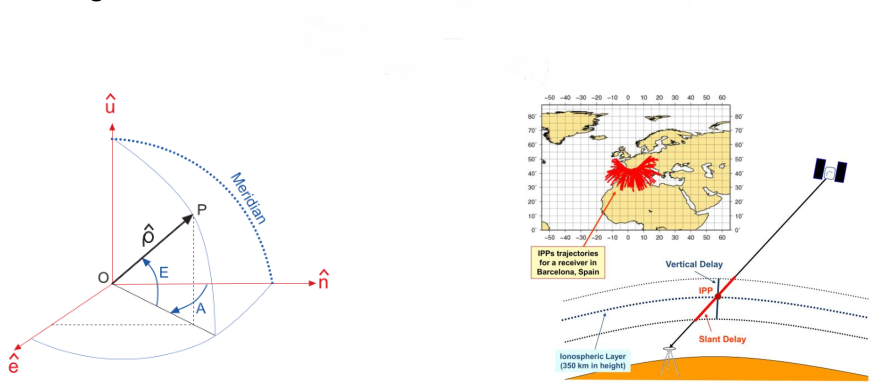
\includegraphics[width=1\textwidth]{elev}
		\caption{Kut elevacije (izvor)}
		\label{fig:elev}
	\end{minipage}
	%	\begin{minipage}{0.9\textwidth}
	%		\centering
	%		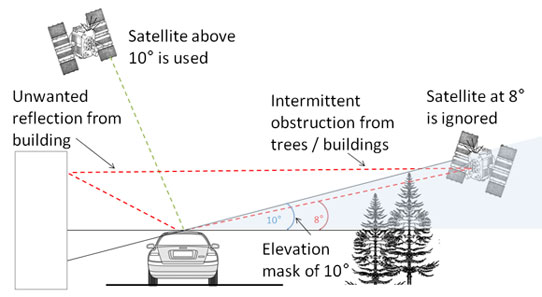
\includegraphics[width=1\textwidth]{elevBetter}
	%		\caption{Kut elevacije u odnosu na prijamnik u automobilu (\url{https://racelogic.support/01VBOX_Automotive/01VBOX_data_loggers/VBOX_3i_Range/VBOX_3i_User_Manual_(All_Variants)/02_-_VB3i_GPS_Antenna_Placement})}
	%		\label{fig:elevBetter}
	%	\end{minipage}
\end{figure}%

Uobičajeni način modeliranja težinskih koeficijenata jednadžbi sustava koristi varijancu $\sigma^2_i$. Ona modelira varijancu slučajnih varijabli mjerenih podataka $i$-te jednadžbe.
Uz pretpostavku neovisnosti mjerenja, svakoj jednadžbi pridružujemo točno jedan težinski koeficijent
definiran izrazom:
\begin{align}
k_i = \frac{1}{\sigma^2_i}
\end{align}
i $W = diag(k_1, k_2, \hdots ,k_N)^{-1}$.

S ciljem uvođenja ovisnosti težinskih koeficijenata o utjecaju ionosfere, 
težine modeliramo pomoću varijanci definiranih preko kuta elevacije.

Uz konzultaciju s literaturom \cite{ref:13,ref:34,ref:4,ref:45,ref:25,LSA:weights} varijancu $i$-te jednadžbe modeliramo pomoću elevacijskog kuta satelita. 
Dobiveni sustav rješavamo korištenjem $QR$ dekompozicije \ref{sec:QR} ili dekompozicije Choleskoga.

Izvodimo tri različita modela težinskih koeficijenata. $k_{ij}$ predstavlja težinski koeficijent $i$-te jednadžbe modeliran na $j$-tim modelom.
\begin{align}\label{eq:elevationTezine1}
k_{i1} = \frac{1}{\sigma^2_{i1}} \\
\sigma^2_{i1} = \frac{1}{ \sin ( Ele_i ) }%
\end{align}
\begin{align}\label{eq:elevationTezine2}
k_{i2} = \frac{1}{\sigma^2_{i2}} \\
\sigma^2_{i2} = 1 + \frac{2}{ \sin ( Ele_i ) }%
\end{align}
\begin{align}\label{eq:elevationTezine3}
k_{i3} = \frac{1}{\sigma^2_{i3}} \\
\sigma^2_{i3} = \frac{1}{ (\sin ( Ele_i) + 0.5)^2 }%
\end{align}
%$\sigma^2_{ij}$ modeliraju varijancu slučajnih varijabli koje opisuju mjerene vrijednosti korištene u konstrukciji $i$-te jednadžbe.
Veći elevacijski kut implicira veći put satelitskog signala kroz ionosferu i pogreška
uzrokovana ionosferom je veća (slika \ref{fig:elev}). Kako elevacijski kut poprima vrijednosti između 0 i $\frac{pi}{2}$, veći elevacijski implicira većom vrijednošću funkcije $\sin^2$ i 
varijance, a manjom vrijednošću težinskog koeficijenta.
Jednadžbe većeg elevacijskog kuta se smatraju manje točnima čemu i težimo.

Sadržaj programskog isječka izvedbe moguće je pronaći u sklopu dodatka \ref{appendix:izvedba}.
Podešavanjem parametra $option \in \{1,2,3\}$ odabire se model težinskih koeficijenata.\\
Podešavanjem parametra $solution \in \{QR,Ch\}$ odabire se model rješavanja sustava jednadžbi, dekompozicijom Choleskoga ili $QR$ dekompozicijom.
Ukoliko se odabere rješavanje dekompozicijom Choleskoga, sustav se rješava računanjem inverza matrice sustava.
Iako se rješavanje sustava računanjem inverza matrice sustava ne smatra dobrim kao izravno rješavanje danog 
sustava, često se koristi u postupcima određivanja položaja $GNSS$ navigacijskim signalima.
Odabirom $QR$ dekompozicije, izbjegava se izravni izračun inverza matrica sustava.
\vspace{0.2cm}\\
Prije pokretanja programskog isječaka potrebno je zadovoljiti uvjete sa stranice \pageref{run:zahtjevi}.
%VIDLJIVO JE DA SE MOŽE DOĆI DO DOBRIH REZULTATA; SAMO JE POTREBNA metoda detekcije završetka rada.
%TRECI NAJBOLJI PA GA ISLI BOLJE ISTRAZITI, promjena eps u veličinu točnosti konvergencije k stvarnoj vrijednosti. 10^3.2  

\chapter{Ocjena kavlitete i zaključci}
\section{Osnovni pristup}
Kvaliteta procjene položaja satelitskim navigacijskim sustavom razmotrena je sa sljedećih stajališta:
\begin{itemize}\label{run:kvaliteta}
	\item Potrebnog računalnog vremena za postizanje stabilne procjene u okruženju R,
	\item Brzine konvergencije iteracijskog postupka u broju iteracija do konvergencije,
	\item Točnosti procjene koordinata položaja.
\end{itemize}
Najbitnijim parametrom sa stajališta navigacije se smatra točnost procjene koordinata položja.\\

Prilikom procjene točnosti, pokreću se različite izvedbe istih datoteka ulaza sadržaja kako je prikazano u dodatku \ref{appendix:izvedba}.
\vspace{0.01cm}
Prvo dajemo ocjenu kvalitete prve izvedbe osnovnog algoritma predočenu tablicom \ref{table:QR} i slikama \ref{fig:1LSAdelta} i \ref{fig:1LSAdeltal10}.%
\begin{table}[H]
	\caption{Kvaliteta prve izvedbe osnovnog algoritma za procjenu položaja u domeni navigacijske primjene}
	%\rowcolors{1}{}{lightgray}
	\begin{center}
		\begin{tabular}{|p{3cm}|p{4cm}|}
			\hline
			\rowcolor{lightgray}NAZIV&   \\
			\rowcolor{lightgray}&   \\
			\multirow{-3}{1cm}{ \cellcolor{lightgray}PARAMETRA} & \multirow{-3}{1cm}{\cellcolor{lightgray}VRIJEDNOST} \\
			\hline
			\vspace{0.1cm}
			vrijeme izvršavanja [s] & \vspace{0.1cm}  52.44 za $10^5$, 24h za $10^10$ iteracija\\
			\vspace{0.1cm}
			broj iteracija do konvergencije & \vspace{0.1cm} $\approx 10^10$ \\
			\vspace{0.1cm}
			točnost procjene [m] & \vspace{0.1cm} $10^3$ \\
			\hline
		\end{tabular}
	\end{center}
	\label{table:QR}
\end{table}
%TO DO na faksu sutra

\begin{figure}[H]
	\begin{minipage}{0.48\textwidth}
		\centering
		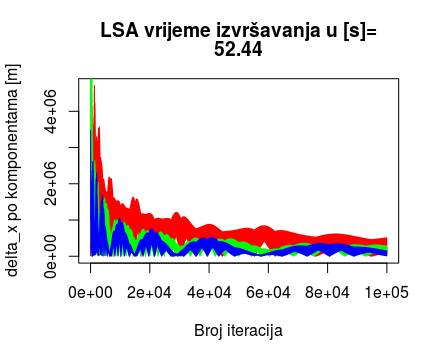
\includegraphics[width=1\textwidth]{1LSAdeltab}
		\caption{Vrijednosti $\Delta \mathbf{x}$ po komponentama kroz iteracije}
		\label{fig:1LSAdelta}
	\end{minipage}%	
	\hspace{1cm}
	\begin{minipage}{0.48\textwidth}
		
		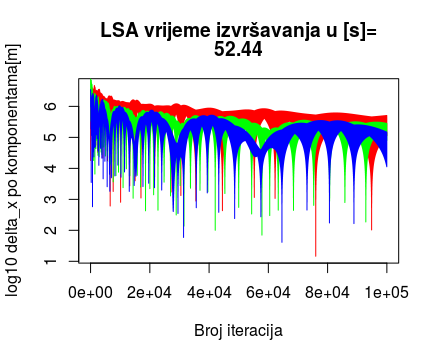
\includegraphics[width=1\textwidth]{1LSAdeltal10b}
		\caption{Logaritam vrijednosti $\Delta \mathbf{x}$ po komponentama kroz iteracije}
		\label{fig:1LSAdeltal10}
	\end{minipage}%
\end{figure}
Na slikama \ref{fig:1LSAdelta} i \ref{fig:1LSAdeltal10} je vidljiv trend smanjivanja izračunate pogreška ($\Delta \mathbf{x}$)  procjene položaja.
U prvih $10^5$ iteracija $\Delta \mathbf{x}$ nikada nije manja od $10^4$ m za sve tri komponente istovremeno.
Još više, $\Delta \mathbf{x}$ je uvijek veće od $10^4$ m u barem dvije komponente, što objašnjava izrazito sporu konvergenciju izvedbe.\\
Smanjujući zahtjeve konvergencije algoritma toliko da proglašavamo konvergenciju ako je barem jedna komponenta $\Delta \mathbf{x}$ manja od $10^2$ ili $10^3$ m,
metoda konvergira u 314, odnosno 195 iteracija. 
\begin{figure}[H]
	\begin{minipage}{0.48\textwidth}
		\centering
		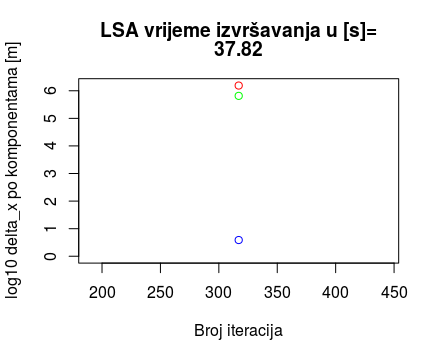
\includegraphics[width=1\textwidth]{1less100deltab}
		\caption{Logaritam vrijednosti komponenata $\Delta \mathbf{x}$ kroz iteracije}
		\label{fig:1less100delta}
	\end{minipage}%	
	\hspace{1cm}
	\begin{minipage}{0.48\textwidth}
		\centering
		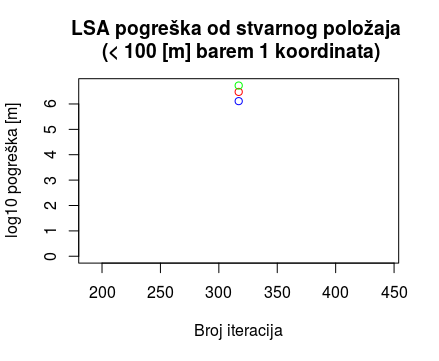
\includegraphics[width=1\textwidth]{1less100realb}
		\caption{Logaritam pogreške određivanja položaja}
		\label{fig:1less100real}
	\end{minipage}%
\end{figure}
Slike \ref{fig:1less100delta} i \ref{fig:1less100real} prikazuju odnos izračunate pogreške u procjeni koordinata i stvarne pogreške u prvoj iteraciji u kojoj je barem jedna komponenta $\Delta \mathbf{x}$
manja od 100 m.

\begin{figure}[H]
	\begin{minipage}{0.48\textwidth}
		\centering
		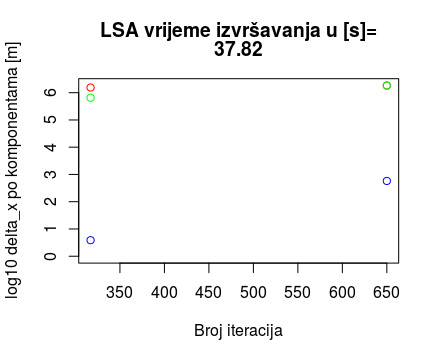
\includegraphics[width=1\textwidth]{1less1000deltab}
		\caption{Logaritam vrijednosti komponenata $\Delta \mathbf{x}$ kroz iteracije }
		\label{fig:1less1000delta}
	\end{minipage}%	
	\hspace{1cm}
	\begin{minipage}{0.48\textwidth}
		\centering
		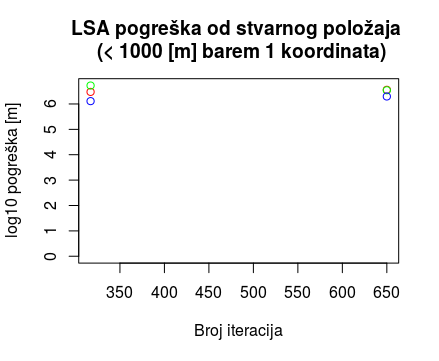
\includegraphics[width=1\textwidth]{1less1000realb}
		\caption{Logaritam pogreške određivanja položaja po komponentama}
		\label{fig:1less1000real}
	\end{minipage}%
\end{figure}

Slike \ref{fig:1less1000delta} i \ref{fig:1less1000real} prikazuju odnos izračunate pogreške u procjeni koordinata i stvarne pogreške komponenti za prvu i drugu iteraciju u kojima je barem jedna komponenta $\Delta \mathbf{x}$
manja od 1000 m.

Promjenjen uvjet konvergencije daje relativno brzu konvergenciju, ali ne i konvergenciju 
prihvatljive točnosti određivanja položaja.
Prava pogreška određivanja položaja nije manja od $10^6$ m.\\


Općenita konvergencija je jako spora, vremenski i u broju iteracija.
Pogreška određivanja položaja dobivena općenitom konvegencijom je zadovoljavajuća, ali nije manja od $10^3$ m.
Dakle, izvedba algoritma zadovoljava kriterij točnosti određivanja položaja, ali ne i 
vremena potrebnog za određivanje položaja. 
\vspace{0.5cm}

Razmotrimo sada drugu izvedbu osnovnog algoritma za procjenu položaja. 
Rezultate ocjene kvalitete su dani tablicom \ref{table:osnovni2izvedba}.
\begin{table}[H]
	\caption{Kvaliteta druge izvedbe osnovnog algoritma za procjenu položaja u domeni navigacijske primjene}
	%\rowcolors{1}{}{lightgray}
	\begin{center}
		\begin{tabular}{|p{3cm}|p{4cm}|}
			\hline
			\rowcolor{lightgray}NAZIV&   \\
			\rowcolor{lightgray}&   \\
			\multirow{-3}{1cm}{ \cellcolor{lightgray}PARAMETRA} & \multirow{-3}{2cm}{\cellcolor{lightgray}VRIJEDNOST} \\
			\hline
			\vspace{0.1cm}
			vrijeme izvršavanja [s] & \vspace{0.1cm}  0.01\\
			\vspace{0.1cm}
			broj iteracija do konvergencije & \vspace{0.1cm} $6$ \\
			\vspace{0.1cm}
			točnost procjene [m] & \vspace{0.1cm} $ > 10^6$ \\
			\hline
		\end{tabular}
	\end{center}
	\label{table:osnovni2izvedba}
\end{table}

\begin{figure}[H]
	\begin{minipage}{0.48\textwidth}
		\centering
		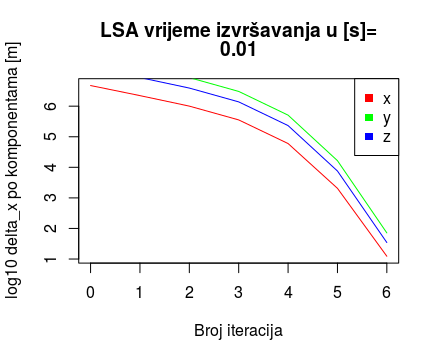
\includegraphics[width=1\textwidth]{2LSAdeltal10b}
		\caption{Logaritam vrijednosti $\Delta x$ po komponentama kroz iteracije}
		\label{fig:2LSAdeltal10}
	\end{minipage}%	
	\hspace{1cm}
	\begin{minipage}{0.48\textwidth}
		
		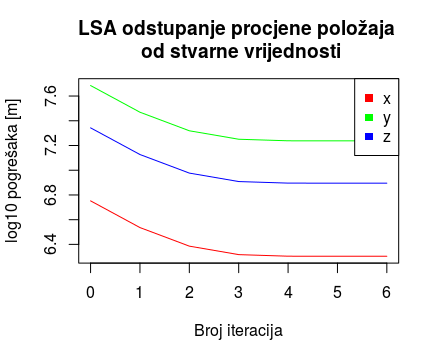
\includegraphics[width=1\textwidth]{2LSAreall10b}
		\caption{Logaritam vrijednosti odstupanja od pravog položaja po komponentama kroz iteracije}
		\label{fig:2LSAreall10}
	\end{minipage}%
\end{figure}

Temeljem slika \ref{fig:2LSAdeltal10} i \ref{fig:2LSAreall10} zaključujemo kako druga izvedba
algoritma \ref{algorithm:iterLSM} brzo konvergira, ali ka krivom rješenju.\\
Dobivena procjena položaja ima odstupanje $> 10^6$ metara.

\subsection{Zaključak} 
Razmatrajući rezultate dvije izvedbe osnovnog algoritma ni jedna u potpunosti ne zadovoljava uvjete
točnosti konvergencije i potrebnog vremena. Prva izvedba konvergira izrazito sporo k
rješenju prihvatljive točnosti, dok druga konvergira brzo, ali ka krivome rješenju.\\
Budući da prilikom ocjene kvalitete izvedbi, na prvo mjesto stavljamo točnost rješenja,
boljom smatramo prvu izvedbu osnovnog algoritma.
Prva izvedba osnovnog algoritma primjenom prvog načina linearizacije je spora i neupotrebljiva kao takva, ali za razuman broj iteracija daje bolju procjenu položaja od druge koja koristi drugi način linearizacije. \\

%KAKVOĆA PREKO RMSE = σ̂^2 = hat(e)^T hat(e)/(N − p) p je broj nepoznatih varijabli 

\section{Poboljšani pristup}
Postoji više inačica izvedbe poboljšanoga pristupa. Odabir se ostvaruje podešavanjima parametara $option$  za odabir modela težinskih koeficijenata i $solution$ za obabir načina rješavanja sustava. (stranica \pageref{eq:elevationTezine1}). Budući da postoje dvije mogućnosti 
odabira za paramatar $solution$ i tri za parametar $option$, svukupno imamo šest inačica izvedbe poboljšanog pristupa.

Ocjene kvalitete različitih inačica izvedbe dane su tablicama \ref{table:3QR} i \ref{table:3Ch} i slikama \ref{fig:3LSA1l10QR}, \ref{fig:3LSA2l10QR}, \ref{fig:3LSA3l10QR}, \ref{fig:3LSA1Ch}, \ref{fig:3LSA2Ch} i \ref{fig:3LSA3Ch}.% 
\begin{table}[H]
	\caption{Ocjene kvalitete izvedbi poboljšanog algoritma za procjenu položaja u domani navigacijske primjene koristeći $QR$ dekompoziciju po modelima težinskih koeficijenata}
	\begin{center}
		\begin{tabular}{||p{3cm}|p{3.1cm}||p{3.1cm}||p{3.1cm}|}
			\hline
			\cellcolor{lightgray} MODEL & 1 & 2 & 3\\
			\hline
			\hline
			\rowcolor{lightgray}NAZIV&   &   &   \\
			\rowcolor{lightgray}&   &   &   \\
			\multirow{-3}{0.5cm}{ \cellcolor{lightgray}PARAMETRA} & \multirow{-3}{0.5cm}{\cellcolor{lightgray}IZNOS} & \multirow{-3}{0.5cm}{\cellcolor{lightgray}IZNOS} & \multirow{-3}{0.5cm}{\cellcolor{lightgray}IZNOS} 
			\\
			\hline
			\vspace{0.1cm}
			vrijeme izvršavanja & \vspace{0.1cm}  0.01 & \vspace{0.1cm} 0.01 &\vspace{0.1cm} 0.01\\
			\vspace{0.1cm}
			broj iteracija do konvergencije &\vspace{0.1cm} 5 &\vspace{0.1cm} 5 &\vspace{0.1cm} 5 \\
			\vspace{0.1cm}
			točnost procjene po koordinatama (x,y,z) & \vspace{0.1cm} $(10,10, < 1)$ &\vspace{0.1cm} $(10,10, < 1)$ &\vspace{0.1cm} $(10,10, < 1)$ \\
			\hline 
		\end{tabular}
	\end{center}
	\label{table:3QR}
\end{table}

\begin{figure}[H]
	\begin{minipage}{0.45\textwidth}
		\centering
		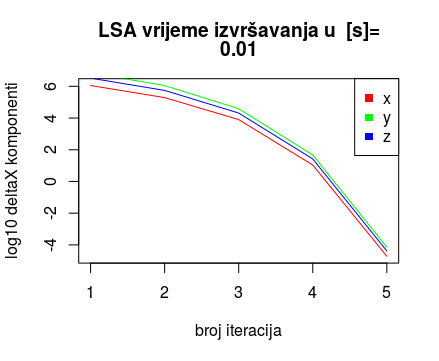
\includegraphics[width=1\textwidth]{3LSAdelta1l10QRb}
		%\caption{Logaritam vrijednosti $\Delta x$ po komponentama kroz iteracije}
		\label{fig:3LSAdelta1l10QR}
	\end{minipage}%	
	\hspace{1cm}
	\begin{minipage}{0.45\textwidth}
		
		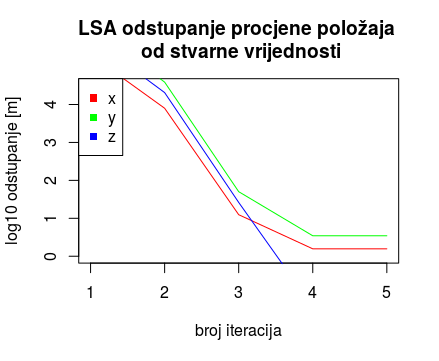
\includegraphics[width=1\textwidth]{3LSAreal1l10QRb}
		%\caption{Logaritam vrijednosti odstupanja od pravog položaja po komponentama kroz iteracije}
		\label{fig:3LSAreal1l10QR}
	\end{minipage}%
	\caption{QR dekompozicija i korištenje prvog modela težinskih faktora}
	\label{fig:3LSA1l10QR}
\end{figure}

\begin{figure}[H]
	\begin{minipage}{0.45\textwidth}
		\centering
		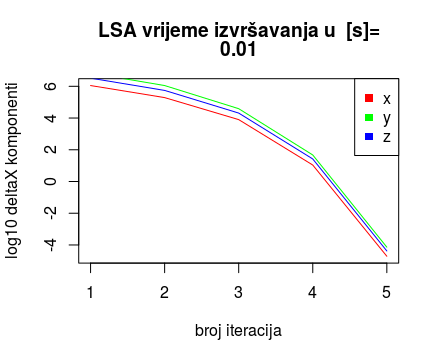
\includegraphics[width=1\textwidth]{3LSAdelta2l10QRb}
		%\caption{Logaritam vrijednosti $\Delta x$ po komponentama kroz iteracije}
		\label{fig:3LSAdelta2l10QR}
	\end{minipage}%	
	\hspace{1cm}
	\begin{minipage}{0.45\textwidth}
		
		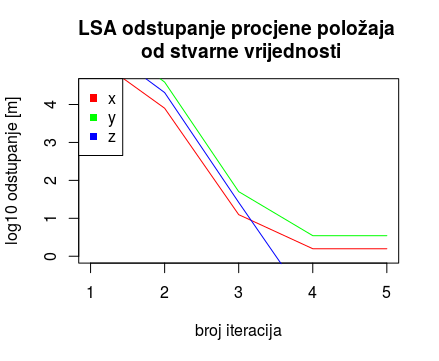
\includegraphics[width=1\textwidth]{3LSAreal2l10QRb}
		%\caption{Logaritam vrijednosti odstupanja od pravog položaja po komponentama kroz iteracije}
		\label{fig:3LSAreal2l10QR}
	\end{minipage}%
	\caption{QR dekompozicija i korištenje drugog modela težinskih faktora}
	\label{fig:3LSA2l10QR}
\end{figure}

\begin{figure}[H]
	\begin{minipage}{0.45\textwidth}
		\centering
		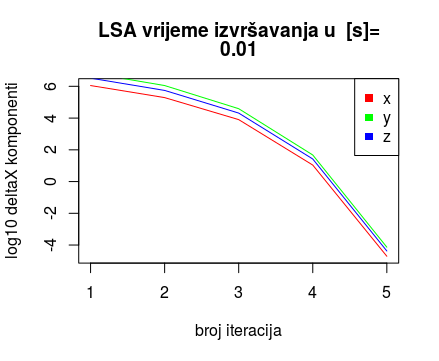
\includegraphics[width=1\textwidth]{3LSAdelta3l10QRb}
		%\caption{Logaritam vrijednosti $\Delta x$ po komponentama kroz iteracije}
		\label{fig:3LSAdelta3l10QR}
	\end{minipage}%	
	\hspace{1cm}
	\begin{minipage}{0.45\textwidth}
		
		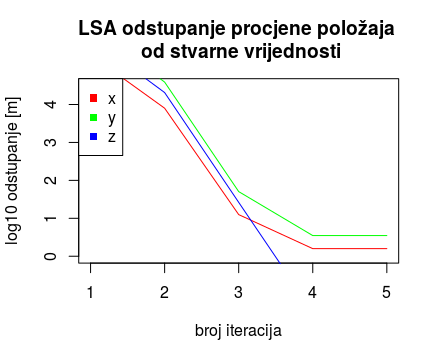
\includegraphics[width=1\textwidth]{3LSAreal3l10QRb}
		%\caption{Logaritam vrijednosti odstupanja od pravog položaja po komponentama kroz iteracije}
		\label{fig:3LSAreal3l10QR}
	\end{minipage}%
	\caption{QR dekompozicija i korištenje trećeg modela težinskih faktora}
	\label{fig:3LSA3l10QR}
\end{figure}
Tablica \ref{table:3QR} i slike \ref{fig:3LSA1l10QR}, \ref{fig:3LSA2l10QR} i \ref{fig:3LSA3l10QR} pokazuju kako nema značajne razlike kvaliteta inačica izvedbi s $QR$ dekompozicijom.\\
%Jedina uočljivija razlika je vrijeme izvršavanja. Naime, korištenje prvog i drugog modela težinskih koeficijenata usporava vrijeme izvaršavanja za 0.01. Ono ne smatramo značajnim, pogotovo ne na ovako malom broju iteracija.

\begin{table}[H]
	\caption{Ocjene kvalitete izvedbi poboljšanog algoritma za procjenu položaja u domeni navigacijske primjene koristeći dekompoziciju Choleskoga po modelima težinskih koeficijenata}
	\begin{center}
		\begin{tabular}{||p{3cm}|p{3.1cm}||p{3.1cm}||p{3.1cm}|}
			\hline
			\cellcolor{lightgray} MODEL & 1 & 2 & 3\\
			\hline
			\hline
			\rowcolor{lightgray}NAZIV&   &   &   \\
			\rowcolor{lightgray}&   &   &   \\
			\multirow{-3}{0.5cm}{ \cellcolor{lightgray}PARAMETRA} & \multirow{-3}{0.5cm}{\cellcolor{lightgray}IZNOS} & \multirow{-3}{0.5cm}{\cellcolor{lightgray}IZNOS} & \multirow{-3}{0.5cm}{\cellcolor{lightgray}IZNOS} 
			\\
			\hline
			\vspace{0.1cm}
			vrijeme izvršavanja & \vspace{0.1cm}  0.12 & \vspace{0.1cm} 0.46 &\vspace{0.1cm} 0.08\\
			\vspace{0.1cm}
			broj iteracija do konvergencije &\vspace{0.1cm} $ 38$ &\vspace{0.1cm} $ 192$ &\vspace{0.1cm} 14 \\
			\vspace{0.1cm}
			točnost procjene po koordinatama (x,y,z) & \vspace{0.1cm} $(10^{3.7},10^{4.3},10^{4})$ &\vspace{0.1cm} $(10^{3.6},10^{4.3},10^{4})$ &\vspace{0.1cm} $(10^{3.6},10^{4.3},10^{4})$ \\
			\hline
		\end{tabular}
	\end{center}
	\label{table:3Ch}
\end{table}

\begin{figure}[H]
	\begin{minipage}{0.48\textwidth}
		\centering
		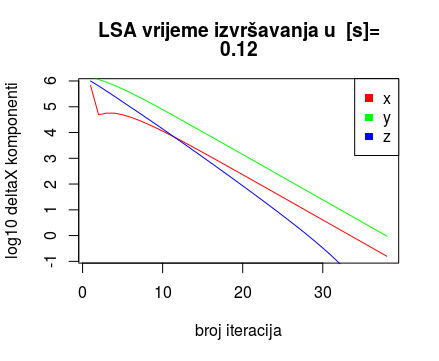
\includegraphics[width=1\textwidth]{3LSAdelta1l10b}
		%\caption{Logaritam vrijednosti $\Delta x$ po komponentama kroz iteracije}
		%\label{fig:3LSAdelta1l10}
	\end{minipage}%	
	\hspace{1cm}
	\begin{minipage}{0.48\textwidth}
		
		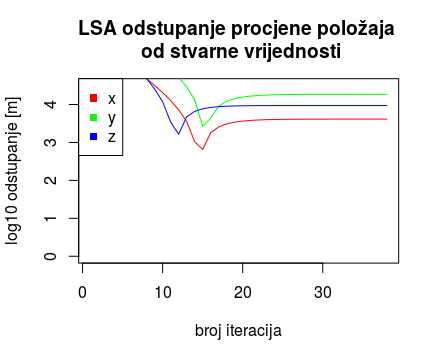
\includegraphics[width=1\textwidth]{3LSAreal1l10b}
		%\caption{Logaritam vrijednosti odstupanja od pravog položaja po komponentama kroz iteracije}
		%	\label{fig:3LSAreal1l10}
	\end{minipage}%
	\caption{Dekompozicija Choleskoga i korištenje prvog modela težinskih faktora}
	\label{fig:3LSA1Ch}
\end{figure}

\begin{figure}[H]
	\begin{minipage}{0.48\textwidth}
		\centering
		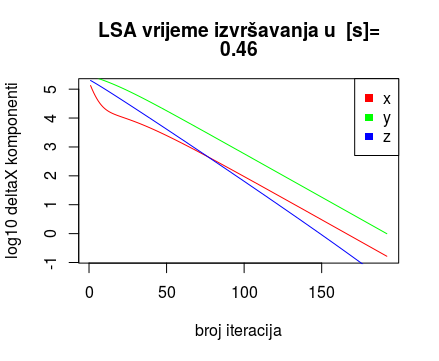
\includegraphics[width=1\textwidth]{3LSAdelta2l10b}
		%\caption{Logaritam vrijednosti $\Delta x$ po komponentama kroz iteracije}
		%\label{fig:3LSAdelta2l10}
	\end{minipage}%	
	\hspace{1cm}
	\begin{minipage}{0.48\textwidth}
		
		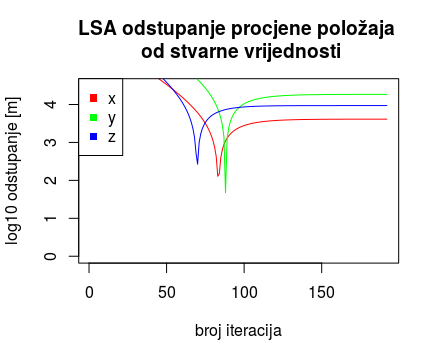
\includegraphics[width=1\textwidth]{3LSAreal2l10b}
		%\caption{Logaritam vrijednosti odstupanja od pravog položaja po komponentama kroz iteracije}
		%\label{fig:3LSAreal2l10}
	\end{minipage}%
	\caption{Dekompozicija Choleskoga i korištenje drugog modela težinskih faktora}
	\label{fig:3LSA2Ch}
\end{figure}

\begin{figure}[H]
	\begin{minipage}{0.48\textwidth}
		\centering
		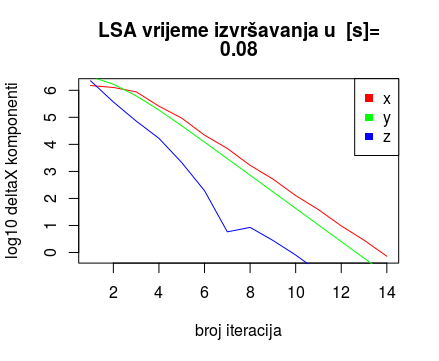
\includegraphics[width=1\textwidth]{3LSAdelta3l10b}
		%\caption{Logaritam vrijednosti $\Delta x$ po komponentama kroz iteracije}
		
	\end{minipage}%	
	\hspace{1cm}
	\begin{minipage}{0.48\textwidth}
		
		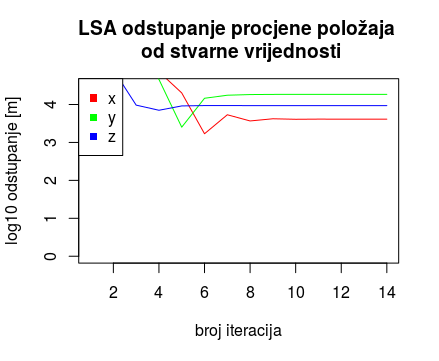
\includegraphics[width=1\textwidth]{3LSAreal3l10b}
		%\caption{Logaritam vrijednosti odstupanja od pravog položaja po komponentama kroz iteracije}
	\end{minipage}%
	\caption{Dekompozicija Choleskoga i korištenje drugog modela težinskih faktora}
	\label{fig:3LSA3Ch}
\end{figure}
Tablica \ref{table:3Ch} i slike \ref{fig:3LSA1Ch}, \ref{fig:3LSA2Ch} i \ref{fig:3LSA3Ch} ne pokazuju razlikovanje u točnosti različitih inačica izvedbi poboljšanog pristupa koje koriste dekompoziciju Choleskoga.

Ukoliko bolje usporedimo lijevi i desni graf svake slike posebno, vidljivo je kako do najmanjeg odstupanja procjene položaja dolazi ne dolazi nakon konvergencije nego ranije.
Prva inačica ima najmanje odstupanje procjene položaja u $(15,15,12)$ iteraciji, druga u $(83,88,70)$, a treća u $(6,5,4)$ po koordinatama. Najmanja odstupanja su jednaka redom $(653.8989, 2684.006, 1645.69)$, $(128.5274,47.26717,267.7062)$ i $(7055.983,2527.817,1696.067)$.
Najbolje najmanje odstupanje ima druga inačica. Ono postiže vrijednost $10^2$ m u najgorem slučaju. 
%Tablica \ref{table:3Ch} i slike \ref{fig:3LSA1Ch}, \ref{fig:3LSA2Ch} i \ref{fig:3LSA3Ch} pokazuju razlikovanje u kvaliteti različitih inačica izvedbi poboljšanog pristupa koje koriste dekompoziciju Choleskoga.
%Korištenje prvog i drugog modela težinskih koeficijenata uzrokuje konvergenciju algoritma,
%ali ne unutar okvira tražene točnosti. Naime, stvarna pogreška određivanja položa je veća od $10^6$. 
%Konvergencija je spora i događa se tek nakon 20000, odnosno 40000 iteracija. Vrijeme izvršavanja je
%znatno dulje nego prilikom koristenja trećeg modela.
%Inačica koja koristi treći model težinskih koeficijenata konvergira već nakon 30 iteracija.
%Nakon konvergencije, odstupanje koordinata položaja prijamnika je zadovoljavajućo. Vrijeme
%izvršavanja je minimalno.\\
%Ukoliko bolje usporedimo lijevi i desni graf sa slike \ref{fig:3LSA3Ch}, vidljivo je kako do najmanjeg odstupanja procjene položaja dolazi od 5. do 15. iteracije, ovisno o koordinati.
%Tada odstupanje za koordinatu koja postiže minimum iznosi manje od $10^3.5$ metara. Nakon što odstupanje dosegne svoj minimum, ono se poveća i stabilizira.
%Dakle, uz danje istraživanje, očekuje se još polje poboljšanje
%u točnosti određivanja položaja.

\subsection{Zaključak}
Budući da se izvedba osnovnog pristupa koja koristi prvi način linearizacije pokazala boljom, 
sve inačice poboljšanog pristupa predstavljaju poboljšanje prve izvedbe osnovnog pristupa.\\
Temeljem rezultata inačica izvedbi poboljšanog pristupa, najbolje se pokazuju inačice koja koriste $QR$ dekompoziciju.
Među njima nema značajnih razlika. Nemogućnost razlikovanja ocjena kvalitete javlja se i zbog izrazito malog broja ostvarenih iteracija.
Naime, mali broj iteracija ne dopušta da se razlike donekle sličnih modela značajno izraze.\\
Rezultati ocjene kvalitete inačica izvedbi koje koriste dekompoziciju Choleskoga nisu prihvatljivi.
Sve inačice konvergiraju k rješenju odstupanja koje nije zadovoljavajuće, ali nije daleko od zadovoljavajućega. Vrijeme izvršavanja je proporcionalno brzini konvergacije.
Također, korištenje dekompozicije Choleskoga pokazuje anomaliju u točnosti određivanja položaja 
kroz iteracije. Postoji zamjetno poboljšanje u točnosti određivanja položaja prije konvergencije algoritma koje se konvergencijom izgubi.
Mogući uzrok značajnog pogoršanja točnosti nakon poboljšanja je korištenje dekompozicije Choleskoga za direktno izračunavanje inverza matrica sustava. Naime, i sama dekompozicija i direktni račun inverza matrica se pokazuju dosta nestabilnima u usporedbi s pripadnim konkurentnim metodama.

\section{Usporedba pristupa i zaključci}
Promatrajući kvalitetu izvedbe pripadnog osnovnog i poboljšanog algoritma, poboljšani algoritam ostvaruje poboljšanje u točnosti procjene položaja, brzini konvergencije i vremenu izvršavanja.

\begin{table}[H]
	\caption{Usporedba pripadnog osnovnog i poboljšanog pristupa za procjenu položaja u domani navigacijske primjene s najmanjim odstupanjem procjene položaja}
	\begin{center}
		\begin{tabular}{||p{3cm}|p{3.1cm}||p{3.1cm}|}
			\hline
			\cellcolor{lightgray} & osnovni & poboljšani\\
			\hline
			\hline
			\rowcolor{lightgray}NAZIV&   &   \\
			\rowcolor{lightgray}&   &   \\
			\multirow{-3}{0.5cm}{ \cellcolor{lightgray}PARAMETRA} & \multirow{-3}{0.5cm}{\cellcolor{lightgray}IZNOS} & \multirow{-3}{0.5cm}{\cellcolor{lightgray}IZNOS} 
			\\
			\hline
			\vspace{0.1cm}
			vrijeme izvršavanja & \vspace{0.1cm}  24h & \vspace{0.1cm} 0.01s \\
			\vspace{0.1cm}
			broj iteracija do konvergencije &\vspace{0.1cm} $10^10$ &\vspace{0.1cm} 5 \\
			\vspace{0.1cm}
			točnost procjene po koordinatama (x,y,z) [m] & $\approx (10^{3},10^{3},10^{4})$ & $(10,10, < 1)$ \\
			\hline
		\end{tabular}
	\end{center}
	\label{table:usporedba}
\end{table}

Poboljšan pristup smanjuje broj iteracija sa $10^{10}$ na svaga 5. Sukladno tome, smanjeno je i vrijeme izvršavanja (tablica \ref{table:usporedba}).
Odstupanje u točnosti je smanjeno za barem dva reda veličine, a u $z$ koordinati i za 4.\\
Pametni odabir modela težinskih koeficijenata poboljšanog algoritma doveo je do poboljšanja u svim  parametrima ocjene kvalitete.
%Za drugu izvedbu
%Iz tablice \ref{table:usporedba} je vidimo kako smanjenje odstupanja uvodi
%neznatno smanjenje broja iteracija. Vremena izračunavanja su jednaka.\\
%Vrijeme i broj iteracija općenito nisu preveliki ni za jednu od gornje dvije izvedbe.
%Daljna analiza rezultata parametara ocjene kvalitete teblice \ref{table:usporedba} ukazuje na brzu konvergenciju iteracijskog postupka u
%osnovnom postupku procjene položaja. U slučaju
%poboljšanog postupka, konvergencija se postiže neznatno ranije, nakon 5 koraka iteracije.


Rezultati ocjena kvaliteta ukazuju kako postoji mogućnost djelotvornog ispravka dijela
slučajnih pogrešaka primjenom poboljšanog postupka procjene položaja.\\
Kako bi primjena poboljšanog algoritma za dovoljno dugački niz pojedinačnih procjena položaja zadovoljila
industrijske zahtjeve, potreno je provesti dodatne validacije i po mogućnosti poboljšati brzinu izvršavanja izvedbe.\\
Danja validacija, razrada i praktične izvedbe navedenih i novih pristupa poboljšanja
ostaju predmet budućih istraživanja.

%%MIAMIAMIA ZAKLJUČAK + summary
%\chapter{Zaključak}
%Satelitska navigacija postala je dio nacionalne infrastrukture te se nalazi u
%temeljima sve brojnijih tehnoloških i društveno-ekonomskih sustava. Korisnička oprema sve je
%izraženije temeljena na konceptu programski određenog radija, što omogućuje fleksibilnost,
%konfigurabilnost i značajno poboljšanje obilježja kvaliltete procjene položaja. 
%Ovim diplomskim radom je prvo predstavljen satelitski navigacijski sustav (GNSS), dan detaljni opis formulacije problema određivanja položaja u domeni navigacijek primjene i mogući smjerovi njegovog rješavanja. Nadalje, predstavljamo GNSS korisničku opremu temeljenu na programski određenom radiju i raspravljamo o izvedbi osnovne i poboljšane inačice algritma za određivanje rješenje problema određivanja položaja. Analiziran je referentni postupak procjene položaja u domeni navigacijske primjene i ograničenja
%njegove primjene. Predložen je poboljšani postupak procjene položaja satelitskim navigacijskim
%sustavom zasnovan na metodi težinskih najmanjih kvadrata.
%Poboljšanje je postignuto djelomičnim slučajnih pogrešaka mjerenja
%pseudoudaljenosti. Svi postupci su izvedeni su u obliku programskih skripti u programskom
%okruženju za statističku analizu, modeliranje, simulacije i računarstvo. Programske izvedbe procjene položaja u okruženju R su validirane na eksperimentalno prikupljenim podatcima.
%Primjena predloženog poboljšananja procjene položaja poboljšala je točnost određivanja
%komponenata položaja. Brzina konvergacije i vrijeme izvršavanja ostaju isti ili neznatno bolji.
%Danja validacija, razrada i praktične izvedbe navedenih i novih pristupa poboljšanja
%ostaju predmet budućih istraživanja.

\bibliographystyle{babamspl} % babamspl ili babplain

% U datoteku diplomski.bib se stavljaju bibliografske reference
% Bibliografske reference u bib formatu se mogu dobiti iz MathSciNet baze, Google Scholara, ArXiva, ...
\bibliography{diplomski}

\pagestyle{empty} % ne zelimo brojanje sljedecih stranica

% I na koncu idu sazeci na hrvatskom i engleskom
\begin{sazetak}
Rastući broj tehnoloških i društveno-ekonomskih sustava se zasniva na satelitskom 
određivanju položaja, npr. snalaženje u prostoru, 
%(2) pronalazak izgubljenih svari, 
 analiza prometnih puteva, pridjeljivanje vremensko-položajnih žigova financijskim transakcijama itd.
Kvaliteta usluge određuje se točnošću procjene položja
satelitskim sustavima.\\
Ovaj rad obuhvaća analizu (referentnog) postupaka procjene položaja u domeni navigacijske primjene te
se otkrivaju potencijalne slabosti i predlaže poboljšanje.
Analiza algoritma uključuje izvedbu i ocjenu kvalitete izvedbe algoritma korištenjem izmjerenih pseudoudaljenosti i programski određenog GPS prijemnika.
Programski određen GPS prijemnik je praktično izveden na osobnom računalu. Korišten je u svrhu obrade prikupljenih opažanja GPS prijemnika u RINEX podatkovnom formatu za ulaz u izvedbe.
Opažanja su prikupljena s referentne međunarodne GNSS stacionarne postaje (engl. International GNSS Service Reference Station, IGS Reference Station) u  Padova, Italija.
Poboljšanja algoritma analizirana su usporednom analizom poboljšanog i izvornog algoritma.
\vspace{0.5cm}

Uvodnim se poglavljem uvodi u svijet globalnih satelitskih navigacijskih sustava (engl. Global Navigation Satellite System, GNSS) te se formuliraju ciljevi rada. Prvo poglavlje detaljnije opisuje jedan odabran GNSS, Globaln pozicijsk sustav (GPS), i uvodi i egzaktno definira problem određivanja položaja u domeni navigacijske primjene. Odabrani GNSS se koristi pri prikupljanju eksperimentalih podataka. \\
Drugo poglavlje opisuje načine pronalaska rješenja problema određivanja položaja definiranog prvim poglavljem.\\
Pri prikupljanju i predobradi eksperimentalih podataka koristi se GNSS korisnička oprema zasnovana na programski određenom radiju.
Opis programski određenog radija i korištene GNSS korisničke opreme nazi se u trećem poglavlju.
Četvrto poglavlja donosi praktičnu izvedbu osnovnog (referentnog) algoritma za procjenu položaja u domeni navigacijske primjene, razloge za njegovo poboljšenje te izvedbu i opis poboljšanja.
Peto poglavlje ocjenjuje i uspoređuje kvalitetu dva izvedena algoritma, osnovnog i poboljšanog, nakon čega slijede zaključci.
\end{sazetak}

\begin{summary}
Satellite positioning has been recognised as an fundamental underlying technology for growing number
of modern technology and socio-economic systems, i.e. orientation in space, traffic routes analysis time and space stamping of financial transactions etc. The quality of services provided by those
systems relies on the satellite positioning performance, especially positioning accuracy. 
This paper covers the analysis of (reference) position estimation procedures in the navigation application domain, discovering of potential weaknesses and suggesting the improvement.
The algorithm analysis involves practical performance and rating of the algorithm performance quality using measured pseudorange and programmable GPS receiver.
A program-specific GPS receiver is practically performed on a personal computer. It was used for processing the GPS receiver's observations in the RINEX data format to form the input of the algorithm performance.
GPS receiver's observations are collected from IGS reference station located in Padua, Italy.
Algorithm enhancements were analyzed by a parallel analysis of the improved and original algorithm.

The introductory chapter introduces the world of global navigation satellite systems (GNSS) and formulates the objectives. Chapter one details a selected GNSS, Global Positioning System (GPS), and introduces and defines the problem of positioning in the navigation application domain.
Selected GNSS is used when collecting experimental data. \\
The second chapter describes solution finding methods of the problem defined by chapter one. \\
GNSS user equipment based on program-specific radio is used when collecting and pre-processing experimental data.
The description of the programmable radio and the GNSS user equipment used are given with the third chapter.
Chapter Four provides a practical performance of the basic (benchmark) algorithm for position assessment in the navigation application domain, the reasons for its improvement and performance and description of the improvement.
The fifth chapter evaluates and compares the quality of two derived algorithms, basic and improved, followed by conclusions. 
\end{summary}

% te zivotopis

\begin{cv}
Mia Filić je rođena u Zagrebu, Republika Hrvatska. Osnovnu i srednju školu je završila u
Sesvetama, Zagreb, Republika Hrvatska u razdoblju od 2000. do 2012. Po završetku srednje škole upisuje, a 2015. završava preddiplomski
studij matematike na Prirodoslovno-matematičkom fakultetu (Matematički odsjek) Sveučilišta u
Zagrebu. Godine 2015. upisuje, a 2017. završava diplomski studij Računarstva i matematike na
Prirodoslovno-matematičkom fakultetu (Matematički odsjek) Sveučilišta u Zagrebu. U sklopu diplomskog studija, zimski
semestar akademske godine 2016/17 provodi na Sveučilištu u Ljubljani, Slovenija u okviru
projekta Erasmus +.
Njezni znanstveni i profesionalni interesi uključuju sljedeća područja: statističko i strojno učenje,
procesiranje signala i navigacijski algoritmi za potrebe satelitske navigacije i programski određenog
radija, detekcija anomalija i modeliranje pogrešaka satelitskog određivanja položaja, kriptografija.
Tokom diplomskog studija uključila se u brojne interne znanstveno-istraživačke projekte, što je
rezultiralo objavom jednog znanstvenog rada u međunarodnom znanstvenom časopisu
TRANSNAV, predstavljanjem šest znanstvenih radova na međunarodnim znanstvenim skupovima i
njihovom objavom u zbornicima s međunarodnom recenzijom, kao i pozvanim predavanjem na
Boston College-u (Boston, MA, SAD) u okviru Međunarodnog skupa UN-a i SAD-a o svemirskoj
meteorologiji i učincima na tehnološke sustave. Mia Filić aktivno djeluje i u području akademskog
obrazovanja, sudjelujući kao pozvani asistent u izvođenju nastave na diplomskom studiju satelitske
navigacije (prema programu UN-a) na Međunarodnoj školi Sveučilišta Beihang za aeronautiku i
astronautiku, Peking, Kina.
Mia Filić je članica (Member) Kraljevskog instituta za navigaciju (The Royal Institut of Navigation,
London, Ujedinjeno Kraljevstvo) te članica Međunarodnog programskog i organizacijskog odbora
znanstvenog skupa Baška GNSS Conference, koja se tradicionalno svakog svibnja održava u Baški,
otok Krk, Republika Hrvatska u organizaciji Kraljevskog instituta za navigaciju.
\end{cv}

\appendix

%\chapter{Taylorov red potencija}\label{appendix:aTay}
%Primjetimo kako smo na stranici \pageref{stranica:NGLin} pretpostavili
%kako će za rezidualnu funkciju $\mathbf{p}(\mathbf{x})$ postojati njezin 
%razvoj u Taylorov red oko svake točke $\mathbf{x_k}$. Ipak,
%Taylorov red nije definiran za svaku funkciju na $\R^n, n \in \N$.
%Prilikom primjene Iterativne metode najmanjih kvadrata, treba zahtjevati da 
%funkcija $\mathbf{p}(\mathbf{x})$ i točka $x_k$ zadovoljava uvjete definicije razvoja funkcije u Taylorov red oko točke $x_k$ \cite{math:tay}.
%\begin{defn}
%	Naka je $f: \mathbf{I} \to \R $ funkcija klase $C^\infty(\mathbf{I})$ definirana
%	na otvorenom intervalu $\mathbf{I} \subseteq \R^n$ i neka je $c \in \mathbf{I}$.
%	Red potencija
%	\begin{align}
%	T \left[f,c\right] := \sum_{n=0}^{\infty} \frac{f^{(n)}}{n!} \left(x - c\right)^n
%	\end{align}
%	nazivamo \textbf{Taylorov red} funkcije $f$ oko točke $c$.
%\end{defn}%
%
%Također,
%pretpostavlja se kako je 
%\begin{align}\label{eg:a1}
%	\mathbf{p}(\mathbf{x_{k+1}}+\Delta \mathbf{x}_k) = T \left[\mathbf{p},x_k \right]
%\end{align}
%što općenito nije točno.
%Naime, Taylorov red $T \left[f,c\right] $ funkcije 
%$f \in C^\infty(\mathbf{I})$ nužno ne konvergira za svaki $x \not = c, x \in \mathbf{I}$
%ili može konvergirati prema nekoj drugoj funkciji.
%Uvjete pod kojima zaista vrijedi \ref{eg:a1} opisani su teoremima u nastavku.
%
%\begin{defn}[Analitička funkcija]
%	Za $f \in C^\infty(\mathbf{I})$ kažemo da je \textbf{analitička u točki} $c \in \mathbf{I}$ ako njezin Taylorov red:
%	\begin{align*}
%		T \left[f,c\right] := \sum_{n=0}^{\infty} \frac{f^{(n)}}{n!} \left(x - c\right)^n
%	\end{align*}
%	
%	ima radijus konvergencije $R > 0$ i ako postoji $0 < \delta \leq R$ takav da vrijedi 
%	\begin{align*}
%	f(x) = T \left[f,c\right] := \sum_{n=0}^{\infty} \frac{f^{(n)}}{n!} \left(x - c\right)^n,
%	\forall x \in \left < c-\delta, c+\delta \right > \cap \mathbf{I}
%	\end{align*}
%	U oznaci: $f \in C^\omega(\mathbf{I})$.
%\end{defn}
%\begin{thm}\label{thm:konv1}
%	Neka je $\sum_{n=0}^{\infty} a_n \left(x - c\right)^n$ red potencija s radijusom konvergencije $R > 0$. Za $\mathbf{I} := \left < c-R, c+R\right >$,
%	funkcija $f: \mathbf{I} \to \R$ definirana s 
%	\begin{align}
%		f(x) := \sum_{n=0}^{\infty} a_n \left(x - c\right)^n
%	\end{align}
%	je analitička na čitavom $\mathbf{I}$. Nadalje, za svaki $\alpha \in \mathbf{I}$ 
%	pripadni Taylorov red
%	\begin{align}
%		T \left[f,\alpha \right] = \sum_{n=0}^{\infty} \frac{f^{(n)}}{n!} \left(x - \alpha \right)^n
%	\end{align}
%	ima radijus konvergencije $\rho \leq R - (c - \alpha)$ i vrijedi 
%	\begin{align}
%	f(x) = T \left[f,\alpha \right] = \sum_{n=0}^{\infty} \frac{f^{(n)}}{n!} \left(x - \alpha \right)^n
%	\end{align}
%\end{thm}
%
%
%\begin{thm}\label{thm:konv}
%	Naka je $f: \mathbf{I} \to \R $ funkcija klase $C^\infty(\mathbf{I})$ definirana
%	na otvorenom intervalu $\mathbf{I} \subseteq \R^n$.
%	Tada je $f \in C^\omega(\mathbf{I}$ ako i samo ako za svaki $c \in \mathbf{I}$ postoje
%	$\delta > 0$ i konstante $C > 0$ i $ r > 0 $ takve da za sve $n \in \Z_+$ vrijedi:
%	\begin{align}
%		\left | f^{n}(x)  \leq  C \frac{n!}{r^n}  \right | 
%		\forall x \in \mathbf{\mathbf{J}} := \left < c-\delta, c+\delta \right > \cap \mathbf{I}
%	\end{align}
%U tom slučaju $f(x) = T \left[f,c\right](x) $ $
%\forall x \in \left < c-r, c+r \right > \cap \mathbf{\mathbf{J}}$.
%\end{thm}
%Za primjenu iterativne metode
%najmanjih kvadrata $\mathbf{p}$ mora biti klase $C^\infty(\mathbf{I})$ gdje je $\mathbf{I}$ unija otvorenih okolina oko svih izračinatih $\mathbf{x}_k, k \in \N$, osim zadnjega.
%Također, otvorena okolina oko $\mathbf{x}_k$  mora barem sadržavaki otvorenu kuglu $K(\mathbf{x}_k,\Delta \mathbf{x}_k)$ i za $\mathbf{p}$ mora vrijediti teorem \ref{thm:konv1} ili  \ref{thm:konv}.

\chapter{Jakobijeva matrica funkcije $\mathbf{h}$, $\mathbf{J}$}
Iz jednakosti \ref{eq:matrix2} i $\mathbf{J} = \mathbf{p}(\mathbf{x})$ dobivamo
\begin{align}
\mathbf{J} = \frac{\partial \mathbf{h}}{\partial \mathbf{x}}
\end{align}
Za 
\begin{align}
\mathbf{h} (\mathbf{x}) := 
\begin{bmatrix}
||(\mathbf{s}_1-\mathbf{x}_{1:3})|| \\
||(\mathbf{s}_2-\mathbf{x}_{1:3})|| \\
||(\mathbf{s}_3-\mathbf{x}_{1:3})||\\
\end{bmatrix} 
\end{align}
dobivamo
\begin{align}
\mathbf{J} = \begin{bmatrix}
\frac{\partial}{\partial \mathbf{x}} ||(s_1-\mathbf{x}_{1:3})|| \\
\frac{\partial}{\partial \mathbf{x}} ||(s_2-\mathbf{x}_{1:3})||\\
\frac{\partial}{\partial \mathbf{x}} ||(s_3-\mathbf{x}_{1:3})|| 
\end{bmatrix}%
= - \begin{bmatrix}
\frac{(s_1-\mathbf{x}_{1:4})^T}{||(s_1-\mathbf{x}_{1:3})||} \\
\frac{(s_2-\mathbf{x}_{1:4})^T}{||(s_1-\mathbf{x}_{1:3})||}\\
\frac{(s_3-\mathbf{x}_{1:4})^T}{||(s_1-\mathbf{x}_{1:3})||} 
\end{bmatrix} = (\mathbf{J}_n(1:3,1:3))
\end{align}
uz $\hat{\mathbf{x}} = \mathbf{x}_n$
\chapter{Mjere kvalitete sazviježđa}\label{appendix:DOP}
Proces određivanja položaja prijamnika je najtočniji ako je međusobni položaj korištenih satelita povoljan.
Kvaliteta međusobanog položaja korištenih satelita ovisi o njohovoj prostornojraspodjeli u odnosu na
položaj prijamnika.
Nepovoljan odnos između satelita rezultira gotovo zavisnim sustavom jednadžbi. 
Što je sustav jednadžbi bliži zavisnome, veća je mogućnost da prilikom procesa određivanja položaja prijamnika sustav zaista i postane zavisan. Zavisnost sustava uzrokovana je pogreškama zaokruživanja. One se mogu smanjiti, ali nikada u potpunosti izbjeći.

Jednim imenom se mjere međusobnog odnosa među satelitima ili mjere kvalitete sazviježđa nazivaju \textit{degradacija točnosti} (\textbf{DOP}, engl. Dilution of precision).
Niske vrijednosti \textbf{DOP}-a znače povoljan, dok 
visoke vrijednosti znače nepovoljan međusobni položaj satelita.
U nastavku navodimo različite \textbf{DOP} mjere \cite{svd_str15}.
Uz%
\begin{align}
\sigma_{0_prior}^2 & := \frac{\mathbf{p_{prior}}^T \mathbf{W}\mathbf{p_{prior}}}{N-4}\\
\mathbf{p_{prior}} & := (p_1(\mathbf{x_0}),p_2(\mathbf{x_0}),p_3(\mathbf{x_0}),p_4(\mathbf{x_0})) \notag \\
\hat{\sigma}_0^2 & := \frac{\mathbf{\hat{p}}^T \mathbf{W}\mathbf{\hat{p}}}{N - 4}
\end{align}
imamo
\begin{align}
\mathbf{Q_{\hat{x}}} & := \hat{\sigma}_0^2(\mathbf{A^1}^T\mathbf{W}\mathbf{A^1})^{-1} \\
\mathbf{Q_{DOP}} & := \frac{\mathbf{Q_{\hat{x}}}}{\hat{\sigma}_0^2 \sigma_{0_prior}^2} \\
& = \frac{(\mathbf{A^1}^T\mathbf{W}\mathbf{A^1})^{-1}}{\sigma_{0_prior}^2} \\
& = \begin{bmatrix}
q_X^2 & q_{YX} & q_{ZX} & q_{d_TX} \\
q_{XY} & q_Y^2 & q_{ZY} & q_{cd_TY} \\
q_{XZ} & q_{YZ} & q_Z^2 & q_{cd_TZ} \\
q_{Xcd_T} & q_{Ycd_T} & q_{Zcd_T} & q_{cd_T}^2 
\end{bmatrix}\\
\mathbf{A^1} & := \begin{bmatrix}
\mathbf{A}[1:N,1:3] & [1 1 1 1]^T
\end{bmatrix}
\end{align}
Prostorna degradacija točnosti određivanja položaja (PDOP, engl. position DOP) je određena izrazom
\begin{align}
PDOP = \sqrt{q_X^2+q_y^2+q_Z^2}
\end{align}
Degradacija točnosti određivanaj vremena (TDOP, engl. time DOP) je određena izrazom
\begin{align}
TDOP = \sqrt{q_{cd_T}^2}
\end{align}
\textbf{DOP} formulacija koja objedunjuje prethodne je geometrijska defradacija točnosti (GDOP, engl. geometric DOP) određena izrazom
\begin{align}
GDOP = \sqrt{q_X^2+q_y^2+q_Z^2+q_{cd_T}^2}
\end{align}
U praksi najčešće promatramo  vrijednosti $PDOP$-a. Vrijednosti $PDOP$-a manje od 2 se smatraju odličnima, između 2 i 4 dobrima, a do 6 prihvatljivima. Vrijednosti iznad 6 su neprihvatljive i sugeriraju nepogodan međusoban položaj satelita.

Dalje definiramo $HDOP$ i $VDOP$. \\
Nakon transformacije gornje lijeve podmatrice matrice $\mathbf{Q-{\hat{x}}}$ veličine $3 \times 3$ iz ECEF XYZ koordinata u ENU koordinate u odnosu na položaj prijamnika, dobivano matricu $\mathbf{Q}_{ENU}$.
\begin{align}
\mathbf{Q}_{DOP,ENU} & := \frac{\mathbf{Q}_{ENU}}{\hat{\sigma}_0^2 \sigma_{0_prior}^2} \\
&=\begin{bmatrix}
q_E^2 & q_{NE} & q_{UE} \\
q_{EN} & q_{N}^2 & q_{UN} \\
q_{EU}^2 & q_{NU} & q_{U}^2 \\
\end{bmatrix}\\
HDOP & := \sqrt{q_E^2 + q_{N}} \\
VDOP & := \sqrt{q_U^2} \\
EDOP & := \sqrt{q_E^2 + q_{N}} \\
NDOP & := \sqrt{q_U^2}
\end{align}
gdje $HDOP$ i $VDOP$ nazivamo horizontalna i vertikalna degradacija točnosti, a
$EDOP$ i $NDOP$ su degradacija točnosti u smeru istoka, odnosno sjevera.

\chapter{Kodovi izvedbe algoritama}\label{appendix:izvedba}
\section{Osnovni pristup}
\subsection{Prvi način linearizacije}
\lstinputlisting[language=R, caption=izvedba1.R, frame=single]{Rsimulation/dipl2.R}%dipl2.R
\subsection{Drugi način linearizacije}
\lstinputlisting[language=R, caption=izvedba2.R]{Rsimulation/dipl1.R}%dipl1.R
\section{Poboljšan pristup: uvođenje težina (WLSM)}
\lstinputlisting[language=R, caption=izvedba3.R]{Rsimulation/dipl4.R}%dipl4.R
\chapter{Sadržaj datoteka ulaza izvedenih algoritama u procesu ocjene kvalitete}\label{appendix:datotekeUlaza}

\begin{figure}[H]
	\caption{Skup mjerenih pseudo-udaljenosti}
	\lstinputlisting[language=R, caption={}]{Rsimulation/pseudorangesa.txt}
\end{figure}
\begin{figure}[H]
	\caption{Skup ispravljenih pseudo-udaljenosti}
	\lstinputlisting[language=R, caption={}]{Rsimulation/pseudorangesb.txt}
\end{figure}
\begin{figure}[H]
	\caption{Skup koordinata položaja satelita u WGS84 koordinatnom sustavu}
	\lstinputlisting[language=R, caption={}]{Rsimulation/satellites.txt}
\end{figure}

%\chapter{Poboljšani pristup s konstantnim težinama}%dipl5.R
%\begin{table}[H]
%	\caption{Ocjene kvalitete izvedbi poboljšanog algoritma za procjenu položaja u domani navigacijske primjene koristeći dekompoziciju Choleskoga i konstantni kut elevacije=0.5707963}
%	\begin{center}
%		\begin{tabular}{||p{3cm}|p{2.1cm}||p{2.1cm}||p{2.1cm}|}
%			\hline
%			\cellcolor{lightgray} MODEL & 1 & 2 & 3\\
%			\hline
%			\hline
%			\rowcolor{lightgray}NAZIV&   &   &   \\
%			\rowcolor{lightgray}&   &   &   \\
%			\multirow{-3}{0.5cm}{ \cellcolor{lightgray}PARAMETRA} & \multirow{-3}{0.5cm}{\cellcolor{lightgray}IZNOS} & \multirow{-3}{0.5cm}{\cellcolor{lightgray}IZNOS} & \multirow{-3}{0.5cm}{\cellcolor{lightgray}IZNOS} 
%			\\
%			\hline
%			\vspace{0.1cm}
%			vrijeme izvršavanja & \vspace{0.1cm}  0.33 & \vspace{0.1cm} 1.25 &\vspace{0.1cm} 0.09\\
%			\vspace{0.1cm}
%			broj iteracija do konvergencije &\vspace{0.1cm} 132 &\vspace{0.1cm} 520 &\vspace{0.1cm} 34 \\
%			\vspace{0.1cm}
%			točnost procjene & \vspace{0.1cm} $\approx 10^{3.4}$ - $10^{4.2}$ &\vspace{0.1cm} $\approx 10^{3.4}$ - $10^{4.2}$ &\vspace{0.1cm} $\approx 10^{3.4}$ - $10^{4.4}$ \\
%			\hline
%			\vspace{0.1cm}
%			točnost najbolje procjene [m] & \vspace{0.1cm} $95.72277 - 1183.634$ &\vspace{0.1cm} $ 21.56159 - 337.3488 $ &\vspace{0.1cm} $ 452.3668 - 7062.732 $ \\
%			\hline
%		\end{tabular}
%	\end{center}
%	\label{table:zanimljivost}
%\end{table}
%
%\begin{figure}[H]
%	\begin{minipage}{0.48\textwidth}
%		\centering
%		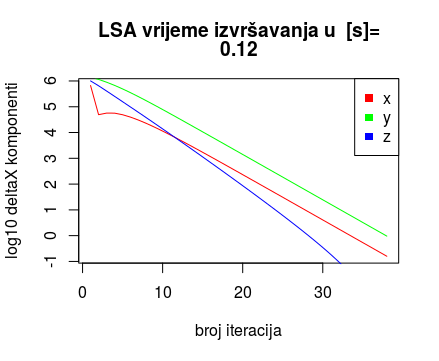
\includegraphics[width=1\textwidth]{3LSAdelta1l10}
%		%\caption{Logaritam vrijednosti $\Delta x$ po komponentama kroz iteracije}
%		\label{fig:3LSAdelta1l10}
%	\end{minipage}%	
%	\hspace{1cm}
%	\begin{minipage}{0.48\textwidth}
%		
%		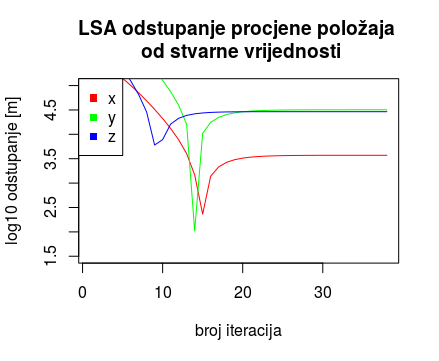
\includegraphics[width=1\textwidth]{3LSAreal1l10}
%		%\caption{Logaritam vrijednosti odstupanja od pravog položaja po komponentama kroz iteracije}
%		\label{fig:3LSAreal1l10}
%	\end{minipage}%
%	\caption{Dekompozicija Choleskoga i korištenje prvog modela težinskih faktora}
%\end{figure}
%
%\begin{figure}[H]
%	\begin{minipage}{0.48\textwidth}
%		\centering
%		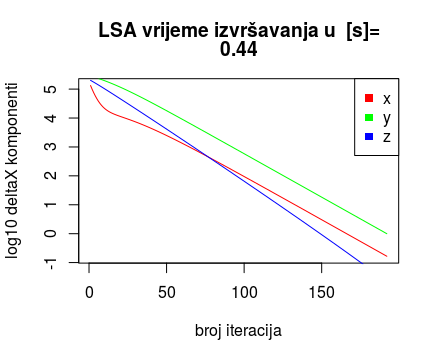
\includegraphics[width=1\textwidth]{3LSAdelta2l10}
%		%\caption{Logaritam vrijednosti $\Delta x$ po komponentama kroz iteracije}
%		\label{fig:3LSAdelta2l10}
%	\end{minipage}%	
%	\hspace{1cm}
%	\begin{minipage}{0.48\textwidth}
%		
%		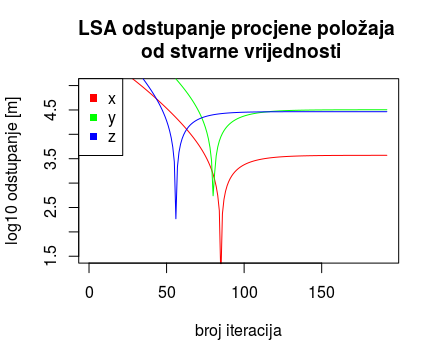
\includegraphics[width=1\textwidth]{3LSAreal2l10}
%		%\caption{Logaritam vrijednosti odstupanja od pravog položaja po komponentama kroz iteracije}
%		\label{fig:3LSAreal2l10}
%	\end{minipage}%
%	\caption{Dekompozicija Choleskoga i korištenje drugog modela težinskih faktora}
%\end{figure}
%
%\begin{figure}[H]
%	\begin{minipage}{0.48\textwidth}
%		\centering
%		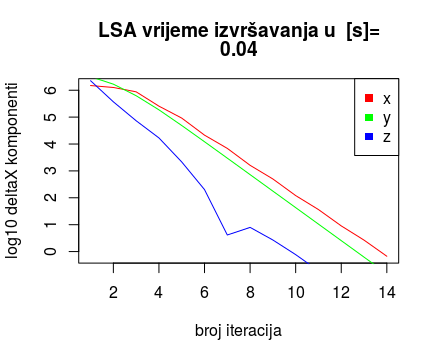
\includegraphics[width=1\textwidth]{3LSAdelta3l10}
%		%\caption{Logaritam vrijednosti $\Delta x$ po komponentama kroz iteracije}
%		\label{fig:3LSAdelta3l10}
%	\end{minipage}%	
%	\hspace{1cm}
%	\begin{minipage}{0.48\textwidth}
%		
%		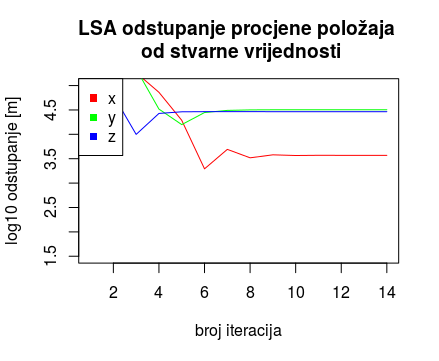
\includegraphics[width=1\textwidth]{3LSAreal3l10}
%		%\caption{Logaritam vrijednosti odstupanja od pravog položaja po komponentama kroz iteracije}
%		\label{fig:3LSAreal3l10}
%	\end{minipage}%
%	\caption{Dekompozicija Choleskoga i korištenje drugog modela težinskih faktora}
%\end{figure}
\end{document}